\documentclass[../BTL.tex]{subfiles}

\begin{document}
\section{ Cài đặt CSDL}
Do sử dụng Spring Data JPA nên việc cài đặt CSDL tương đối đơn giản, chỉ việc cài MySQL Server và MySQL Workbench để làm việc với MySQL trên giao diện đồ họa và tạo cơ sở dữ liệu mới và viết vào trong file cấu hình của backend là application.properties

Đối với việc triển khai trên môi trường web, nhóm em dùng Aiven - Aiven cung cấp 1 server MySQL miễn phí có giới hạn nên nhóm em sẽ tạo trên giao diện web và có được các cấu hình như trên hình \ref{fig:aiven-mysql-config}, sau đó viết các cấu hình này trong file application.properties để backend có thể kết nối với cơ sở dữ liệu


Cấu hình trong file application.properties cụ thể như sau:
\begin{verbatim}
spring.datasource.url=
spring.datasource.username=
spring.datasource.password=
\end{verbatim}

\begin{figure}
    \centering
    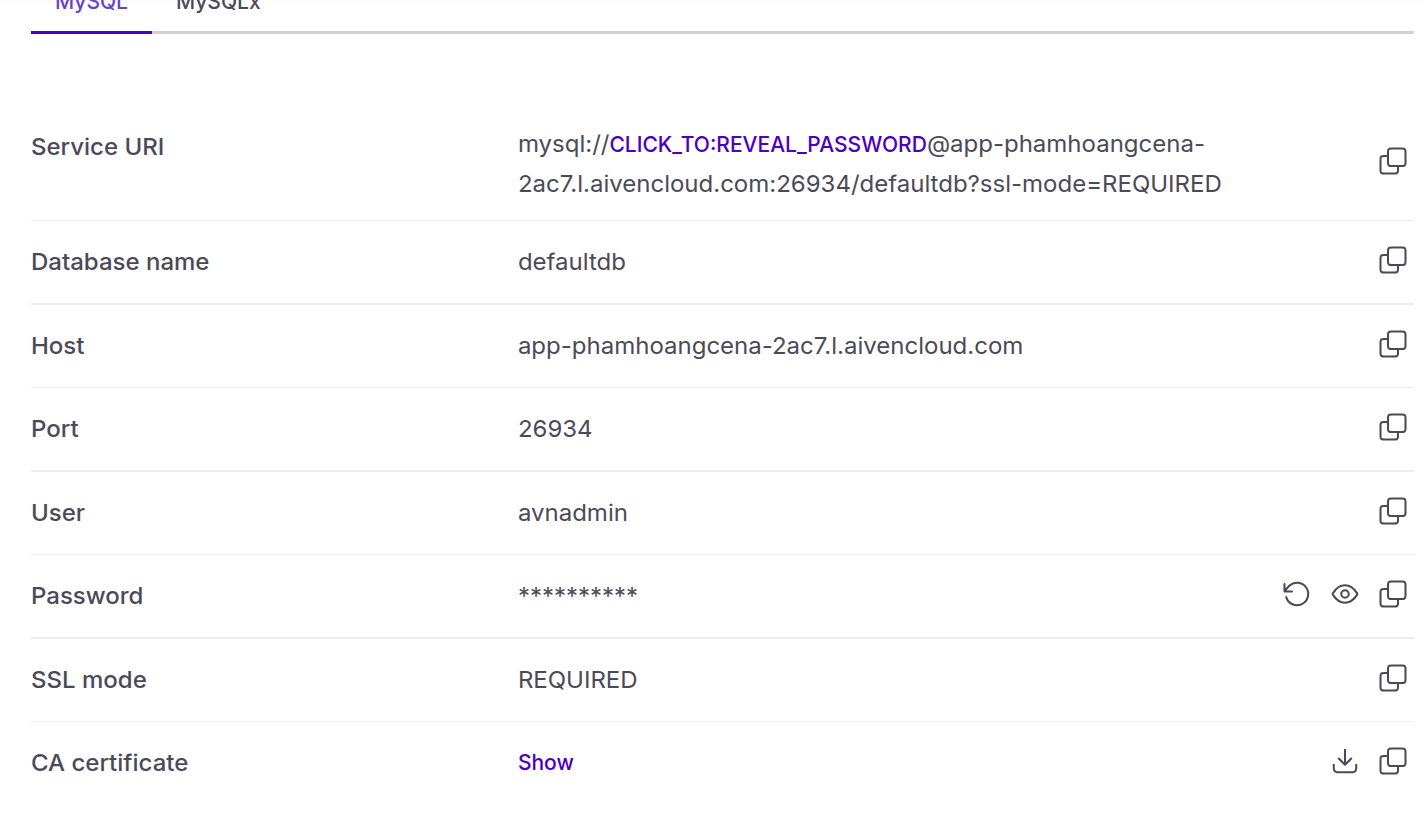
\includegraphics[width=1\linewidth]{Hinhve/aiven-mysql-config.png}
    \caption{ Cấu hình cơ sở dữ liệu MySQL trên Aiven}
    \label{fig:aiven-mysql-config}
\end{figure}
\section{ Cài đặt giả lập môi trường server hosting}
\subsection{ Cài đặt giả lập môi trường server hosting backend}
Để giả lập môi trường server hosting thì nhóm em sử dụng công cụ Docker, đầu tiên với bên backend, do dùng công cụ xây dựng là Maven, sau khi lập trình và khai báo file pom.xml thì tiến hành thực hiện lệnh 'mvn clean package' sẽ thực hiện việc đóng gói dự án thành file jar để có thể chạy file jar này để chạy dự án, kết quả là sẽ có được file jar như trên hình \ref{fig:mvn-clean-package}.

\begin{figure}
    \centering
    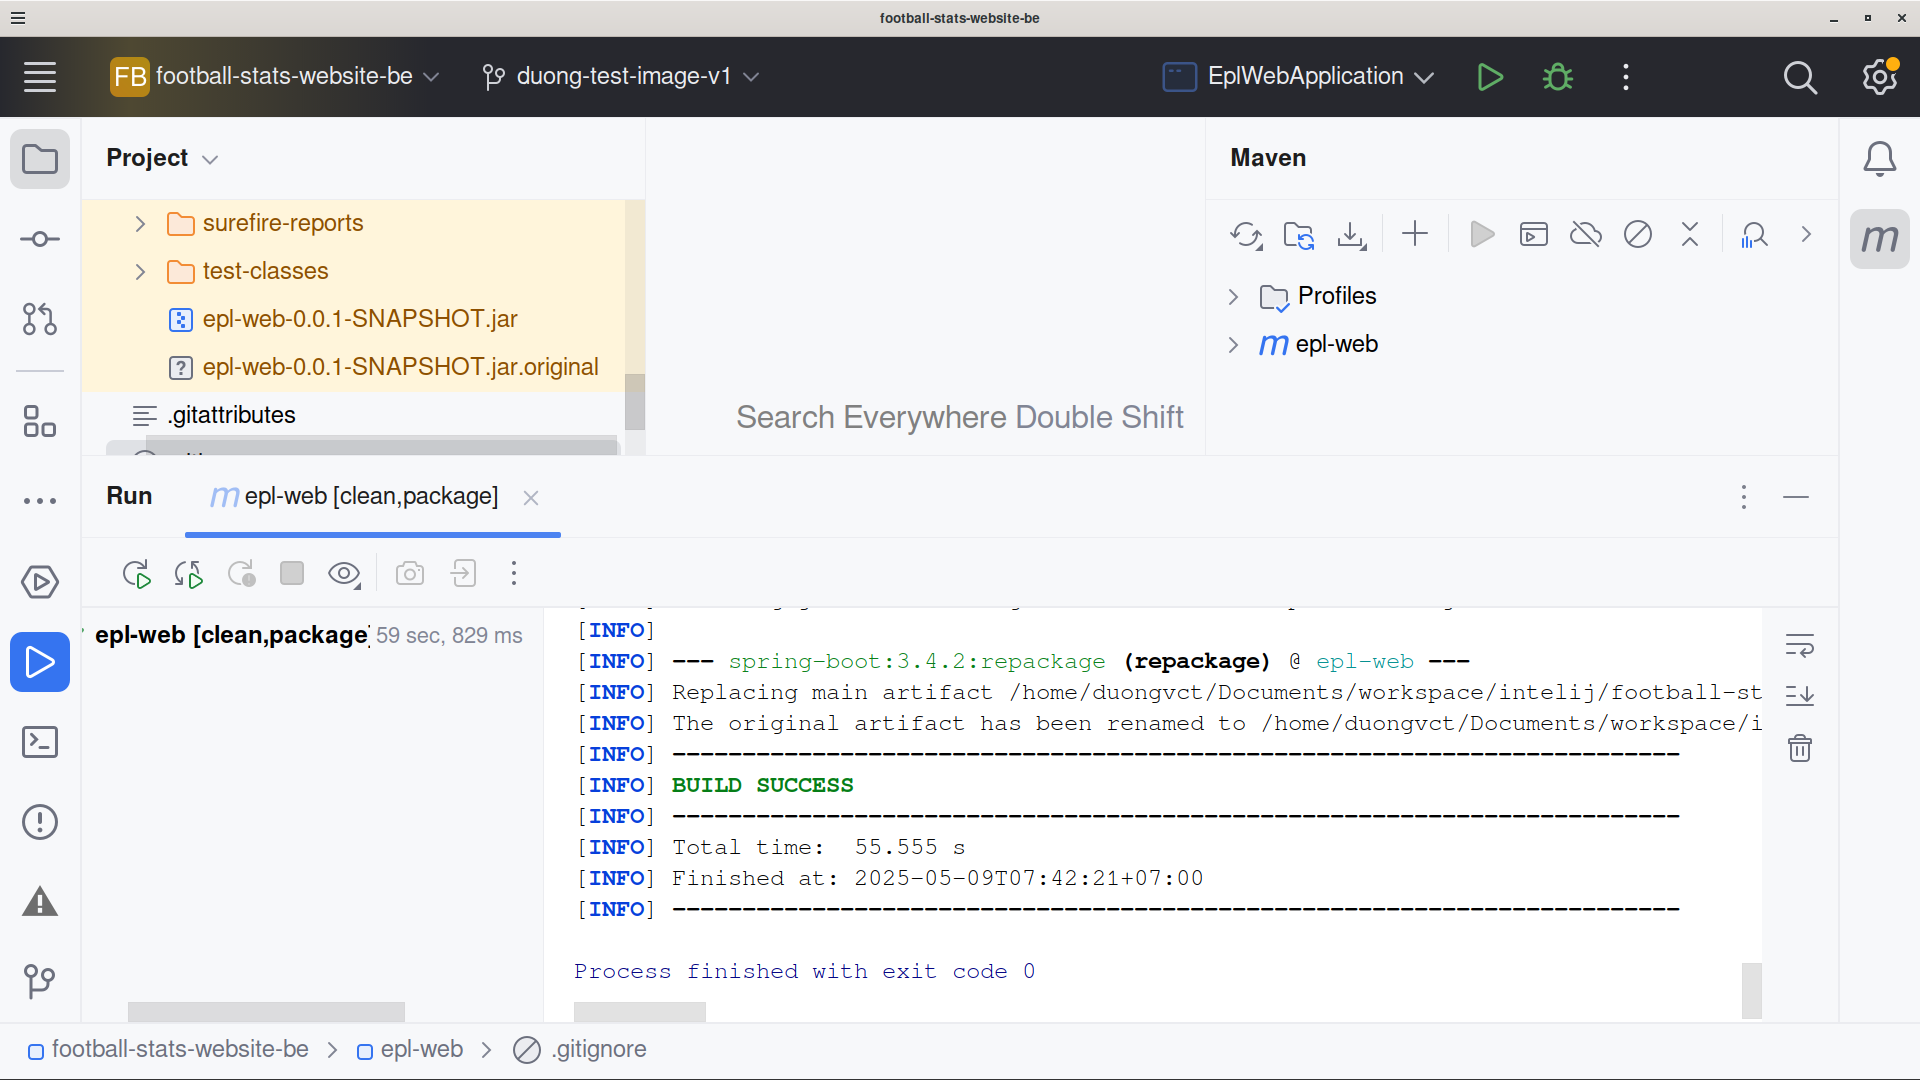
\includegraphics[width=1\linewidth]{Hinhve/mvn-clean-package.png}
    \caption{ Kết quả sau khi chạy mvn clean package}
    \label{fig:mvn-clean-package}
\end{figure}


Sau đó đến bước viết Dockerfile để cấu hình cho docker images mà sau này sẽ được triển khai trên web. File Dockerfile được viết như sau:
\begin{verbatim}
FROM eclipse-temurin:21-jre
WORKDIR /app
RUN groupadd -r appuser && useradd -r -g appuser appuser
COPY epl-web/target/*.jar app.jar
RUN chown -R appuser:appuser /app
USER appuser
EXPOSE 8080
ENV JAVA_OPTS="-Xmx512m -Xms256m"
ENTRYPOINT java $JAVA_OPTS -jar app.jar
\end{verbatim}

Sau đó, để xây dựng Docker image thì chỉ cần chạy lệnh 
'docker build -t dockerhub\_username/epl-web:latest .' tại đường dẫn chứa file Dockerfile với dockerhub\_username chính là username tài khoản trên Dockerhub , kết quả của bước này như trên hình \ref{fig:docker-build-be1} và hình \ref{fig:docker-build-be2}. Để chạy thì ta sẽ chạy lệnh ánh xạ cổng như sau: 'docker container run -p 8080:8080 dockerhub\_username/epl-web:latest' để chạy Docker image trong Docker container, , kết quả như trên hình \ref{fig:docker-container-run-be1} và hình \ref{fig:docker-container-run-be2}. Sau đó chỉ cần truy cập địa chỉ 'http://localhost:8080' để truy cập phần backend. Để triển khai thì sau khi xây dựng Docker image sẽ thực hiện việc đẩy lên Dockerhub: thực hiện lệnh 'docker push dockerhub\_username/epl-web:latest' và đăng nhập vào Dockerhub để đẩy lên Dockerhub, kết quả của bước này như trên hình \ref{fig:docker-push-be}

\subsection{ Cài đặt giả lập môi trường server hosting frontend}
Tiếp theo đến frontend, nhóm em sử dụng React và Nginx để triển khai trên Render, do đó file Dockerfile bên phía frontend như sau:

\begin{verbatim}
# Stage 1: Build the React app
FROM node:20-alpine AS builder

WORKDIR /app

COPY package*.json ./
RUN npm install

COPY . .
RUN npm run build

# Stage 2: Serve with nginx
FROM nginx:alpine

# Remove default nginx static assets
RUN rm -rf /usr/share/nginx/html/*

# Copy built assets from builder
COPY --from=builder /app/dist /usr/share/nginx/html

# Copy custom nginx config if needed (optional)
# COPY nginx.conf /etc/nginx/conf.d/default.conf

EXPOSE 80

CMD ["nginx", "-g", "daemon off;"]
\end{verbatim}

và với câu lệnh tương tự phía backend để xây dựng image và chạy image trong container cũng như đẩy lên trên Dockerhub. Cụ thể, để xây dựng image thì nhập lệnh 'docker build -t dockerhub\_username/epl-web-fe:latest .', kết quả như trên hình \ref{fig:docker-build-fe1}, \ref{fig:docker-build-fe2} và hình \ref{fig:docker-build-fe3}. Để chạy container thì chạy lệnh 'docker container run -p 5173:80 dockerhub\_username/epl-web-fe:latest', kết quả như trên hình \ref{fig:docker-container-run-fe} và truy cập đường dẫn 'http://localhost:5173' để truy cập giao diện frontend và sử dụng. Để đẩy lên dockerhub thì chạy lệnh 'docker push dockerhub\_username/epl-web-fe:latest', kết quả như trên hình \ref{fig:docker-push-fe}.
\begin{figure}
    \centering
    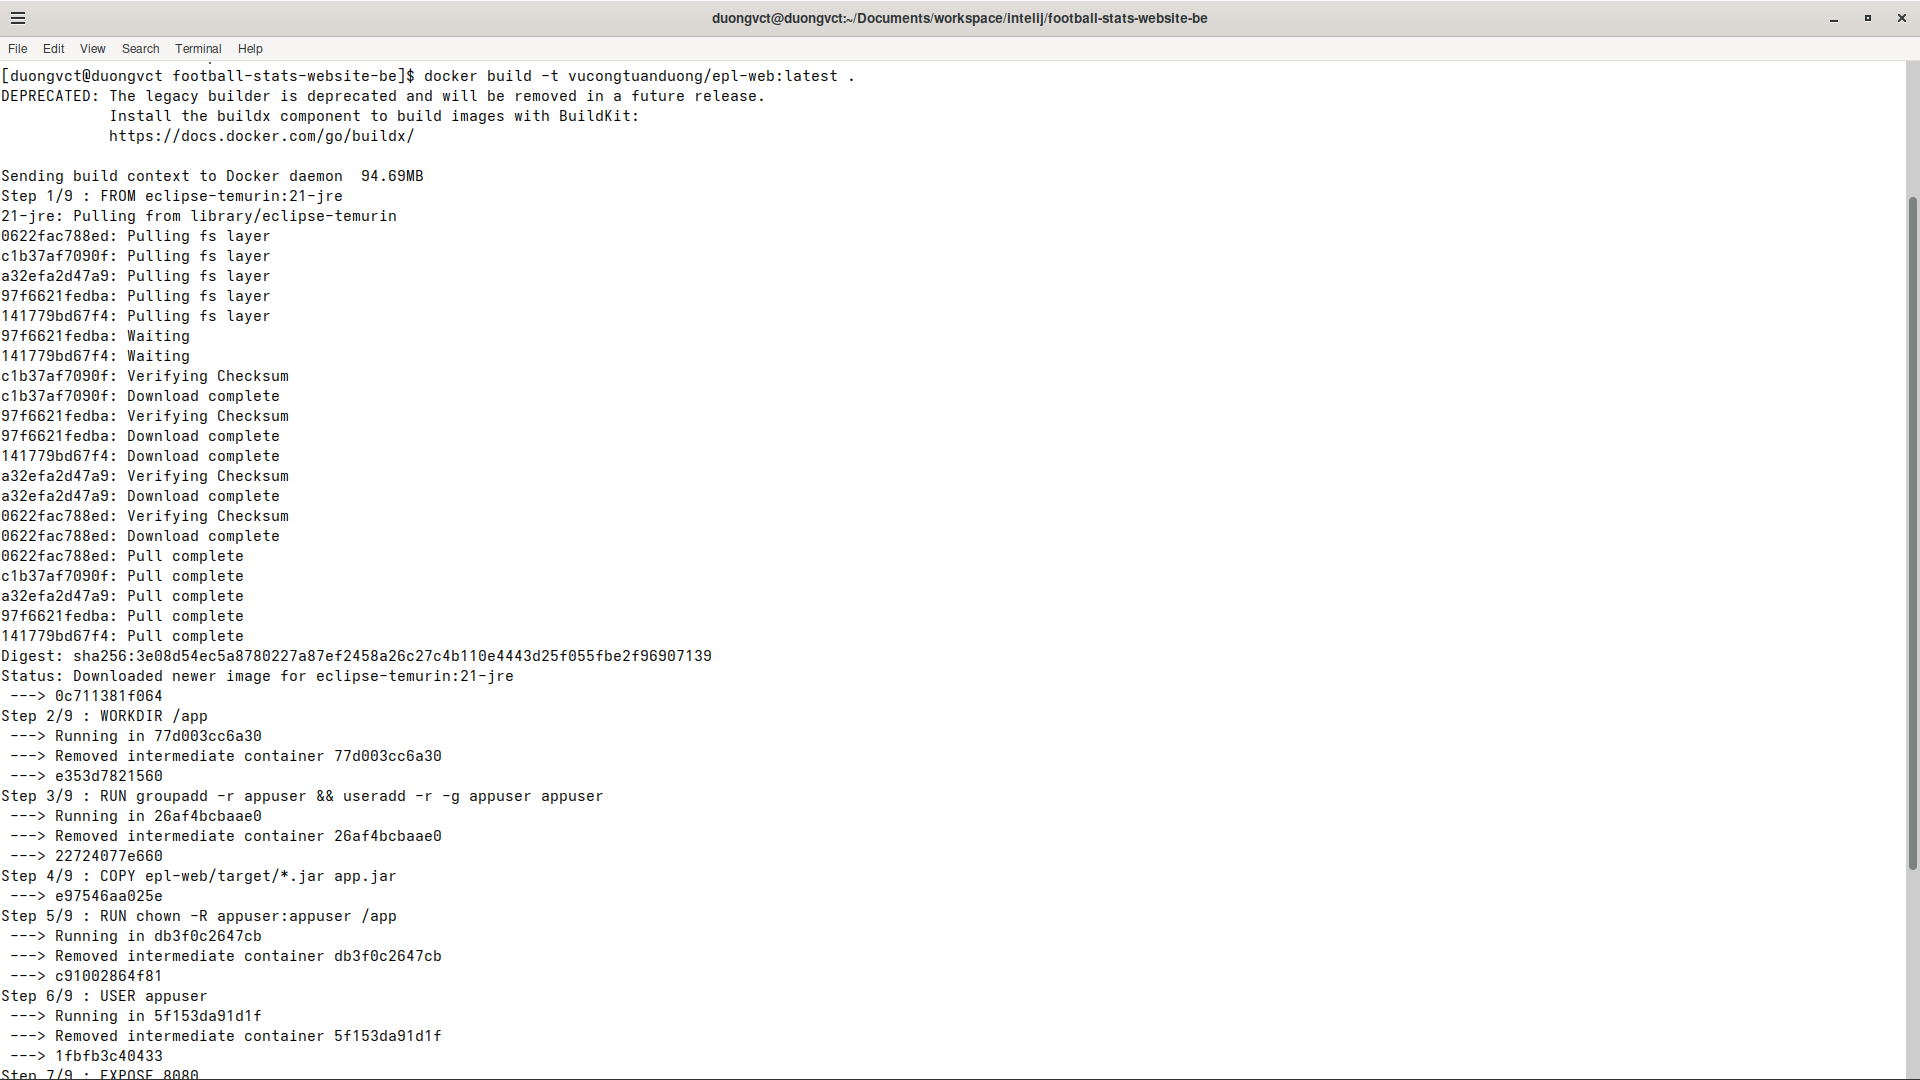
\includegraphics[width=1\linewidth]{Hinhve/docker-build-be1.png}
    \caption{ Kết quả build Docker image phía backend - ảnh 1}
    \label{fig:docker-build-be1}
\end{figure}
\begin{figure}
    \centering
    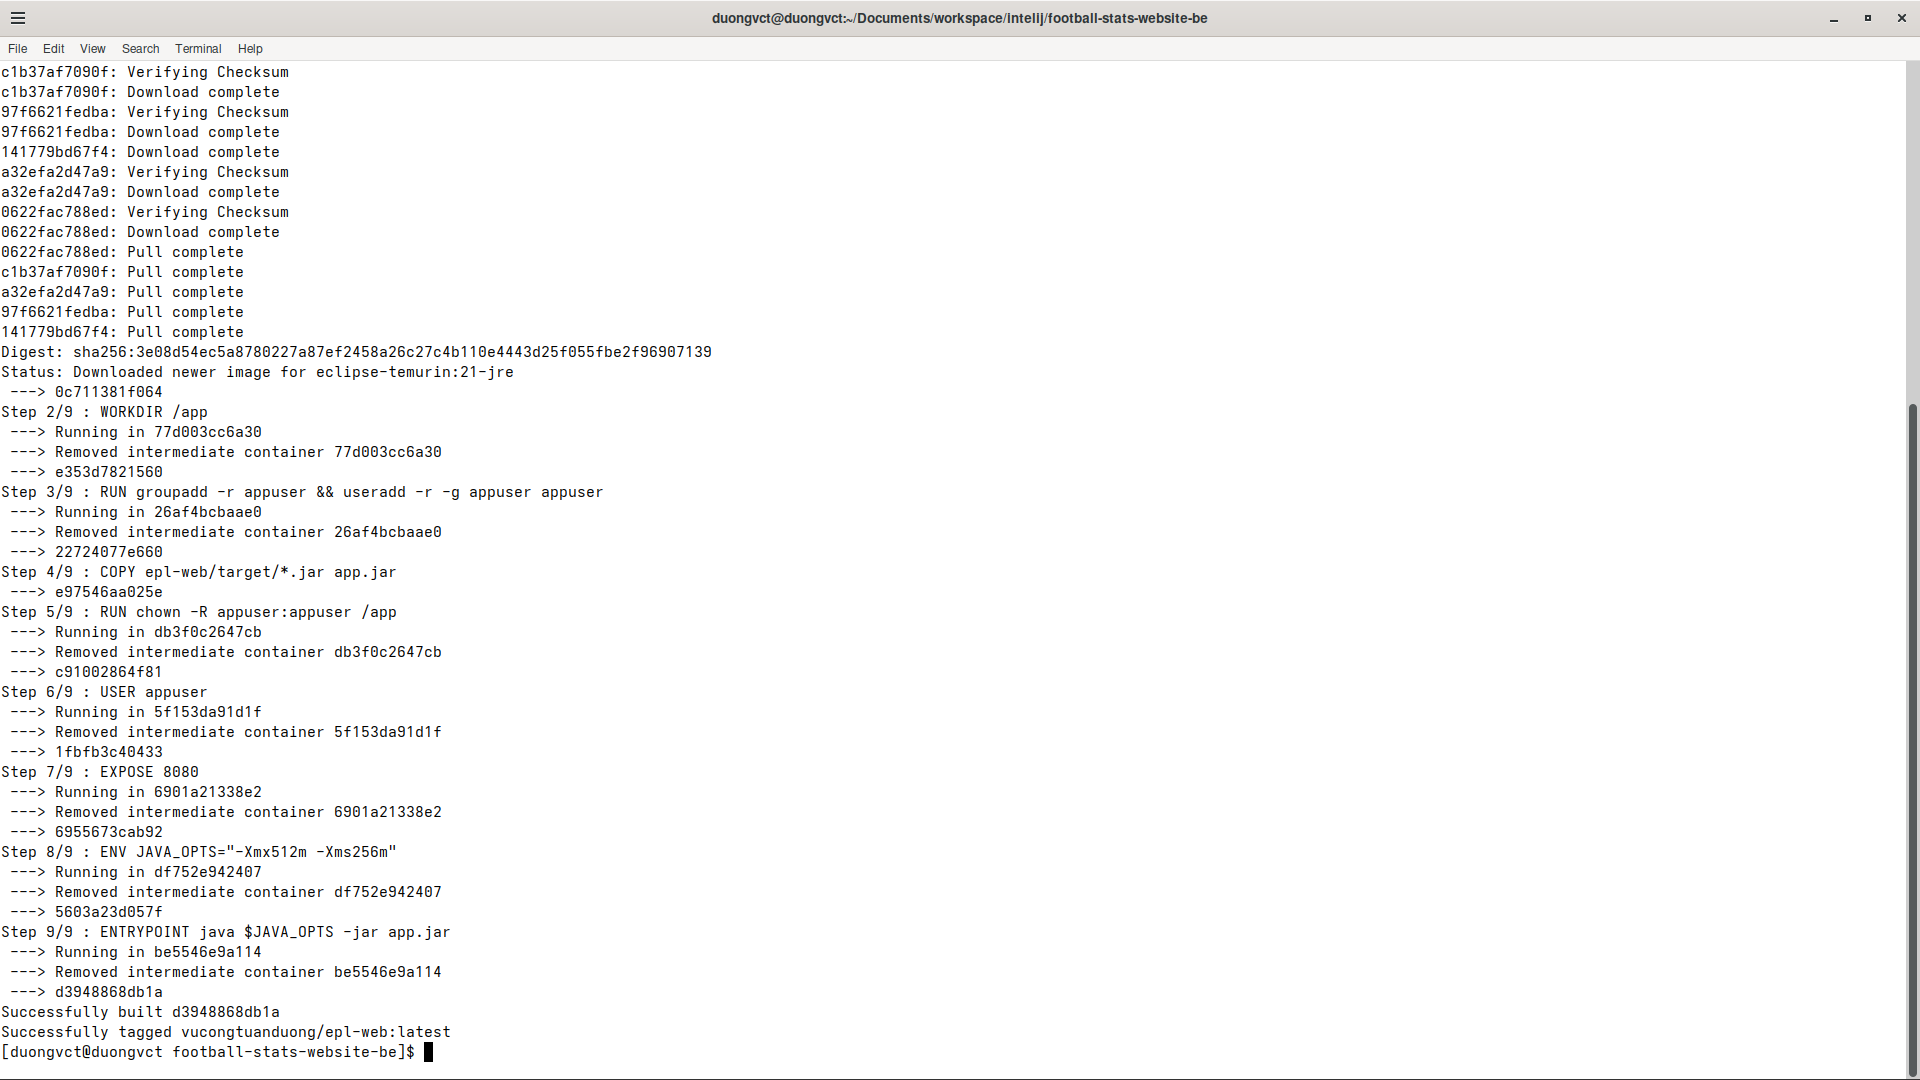
\includegraphics[width=1\linewidth]{Hinhve/docker-build-be2.png}
    \caption{Kết quả build Docker image phía backend - ảnh 2}
    \label{fig:docker-build-be2}
\end{figure}
\begin{figure}
    \centering
    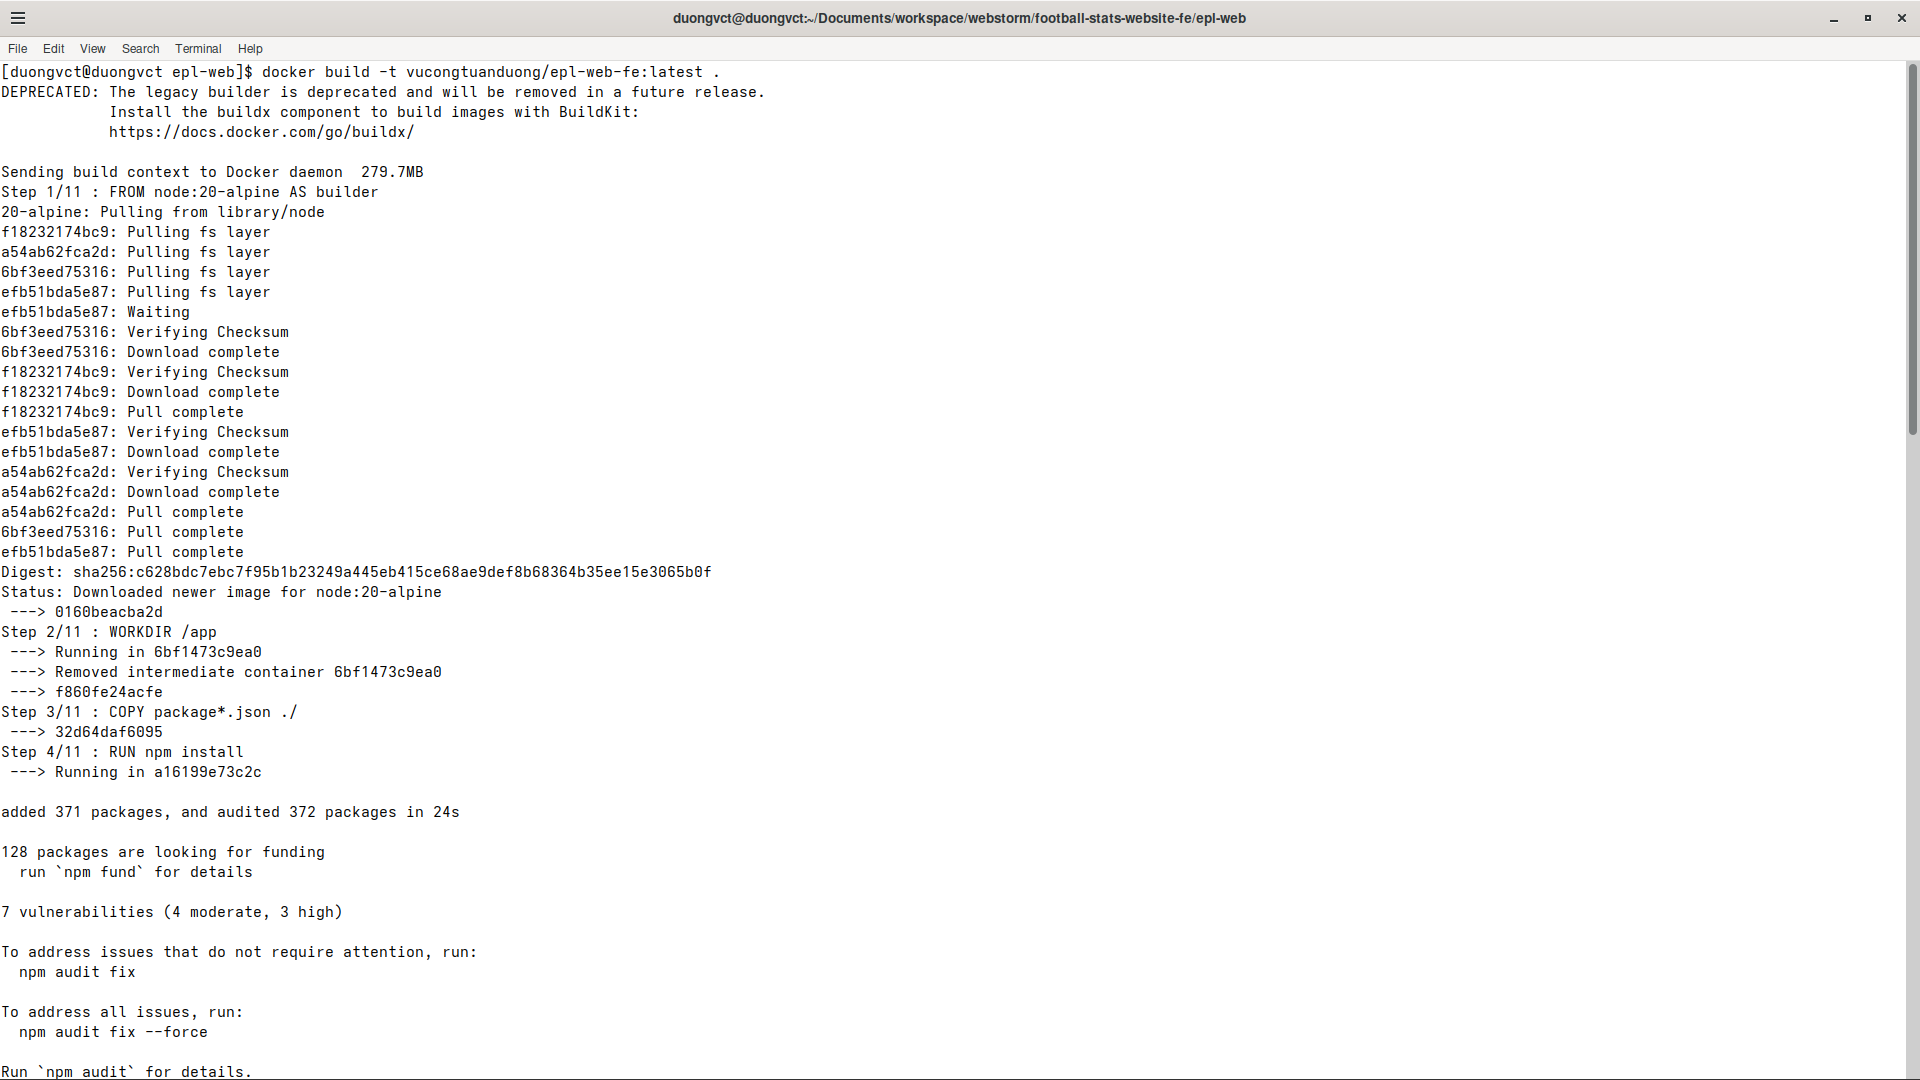
\includegraphics[width=1\linewidth]{Hinhve/docker-build-fe1.png}
    \caption{Kết quả build Docker image phía frontend - ảnh 1}
    \label{fig:docker-build-fe1}
\end{figure}
\begin{figure}
    \centering
    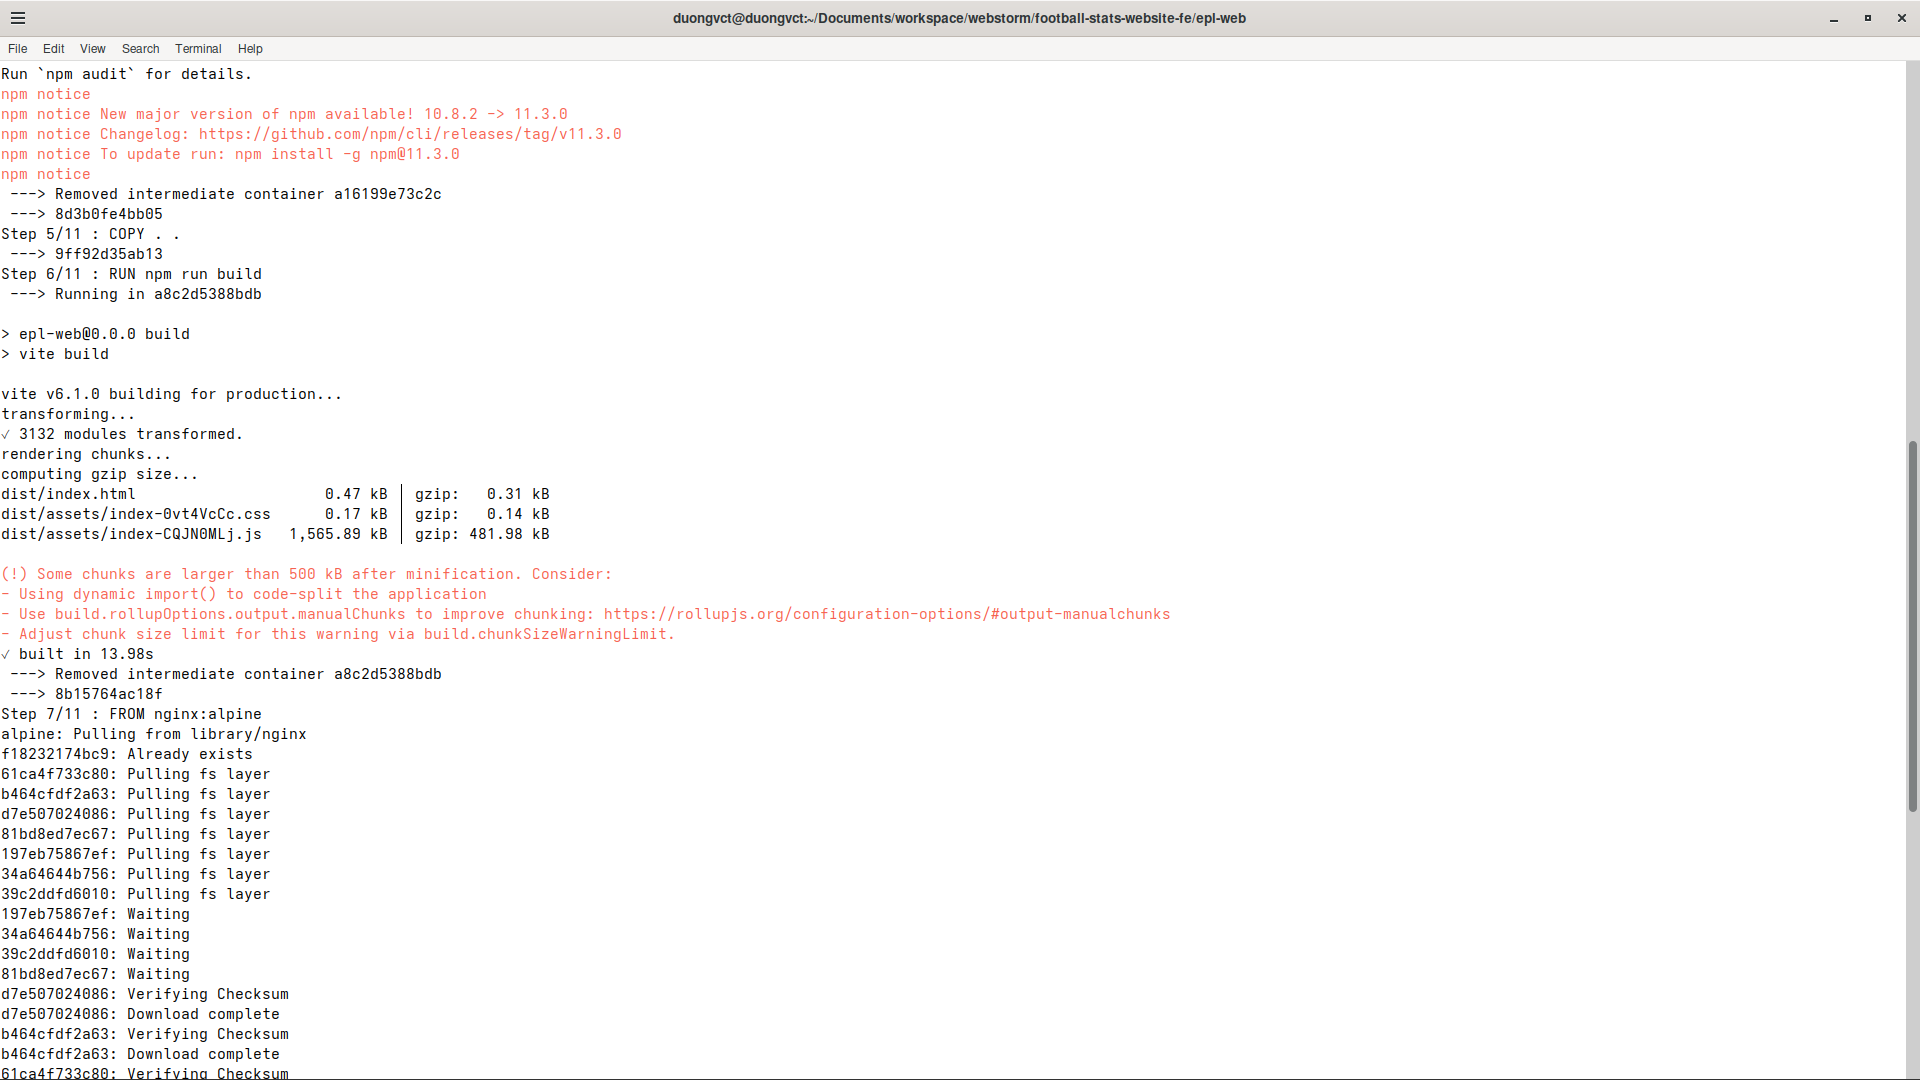
\includegraphics[width=1\linewidth]{Hinhve/docker-build-fe2.png}
    \caption{Kết quả build Docker image phía frontend - ảnh 2}
    \label{fig:docker-build-fe2}
\end{figure}
\begin{figure}
    \centering
    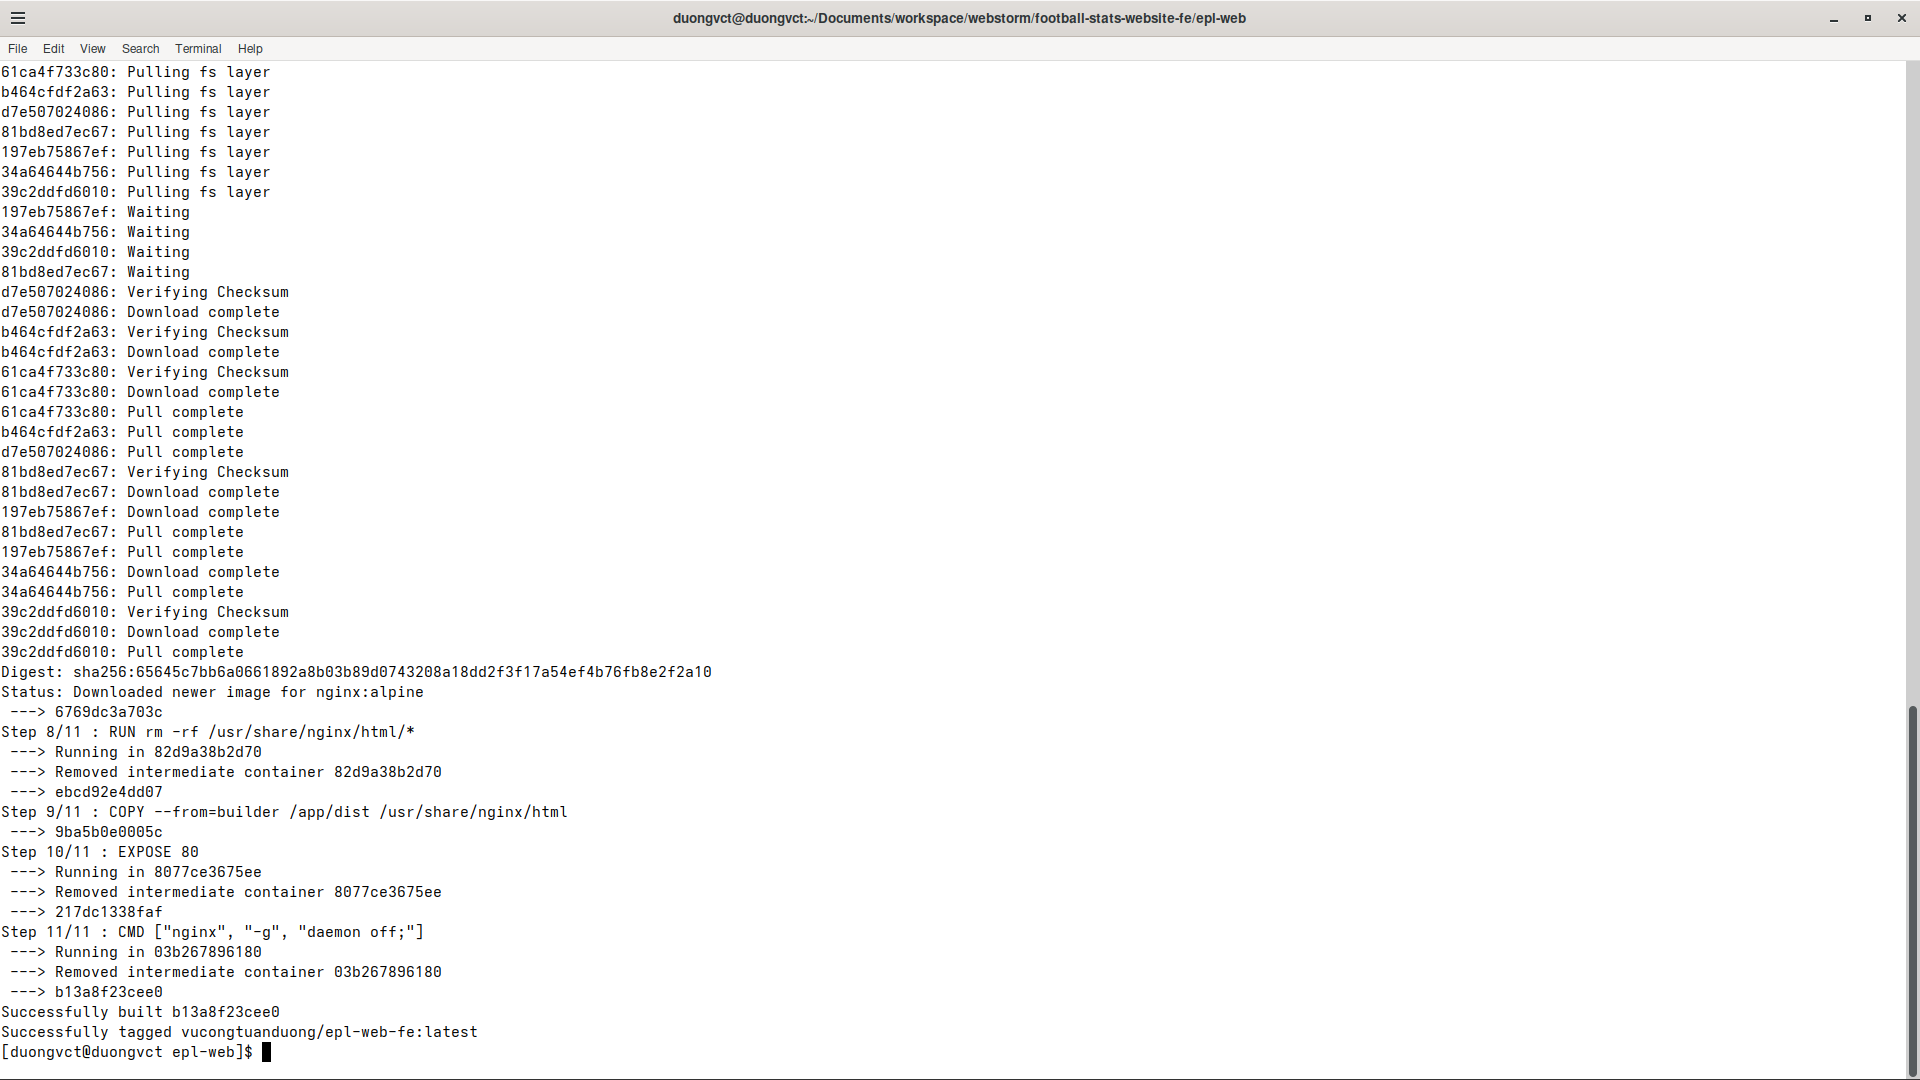
\includegraphics[width=1\linewidth]{Hinhve/docker-build-fe3.png}
    \caption{Kết quả build Docker image phía frontend - ảnh 3}
    \label{fig:docker-build-fe3}
\end{figure}
\begin{figure}
    \centering
    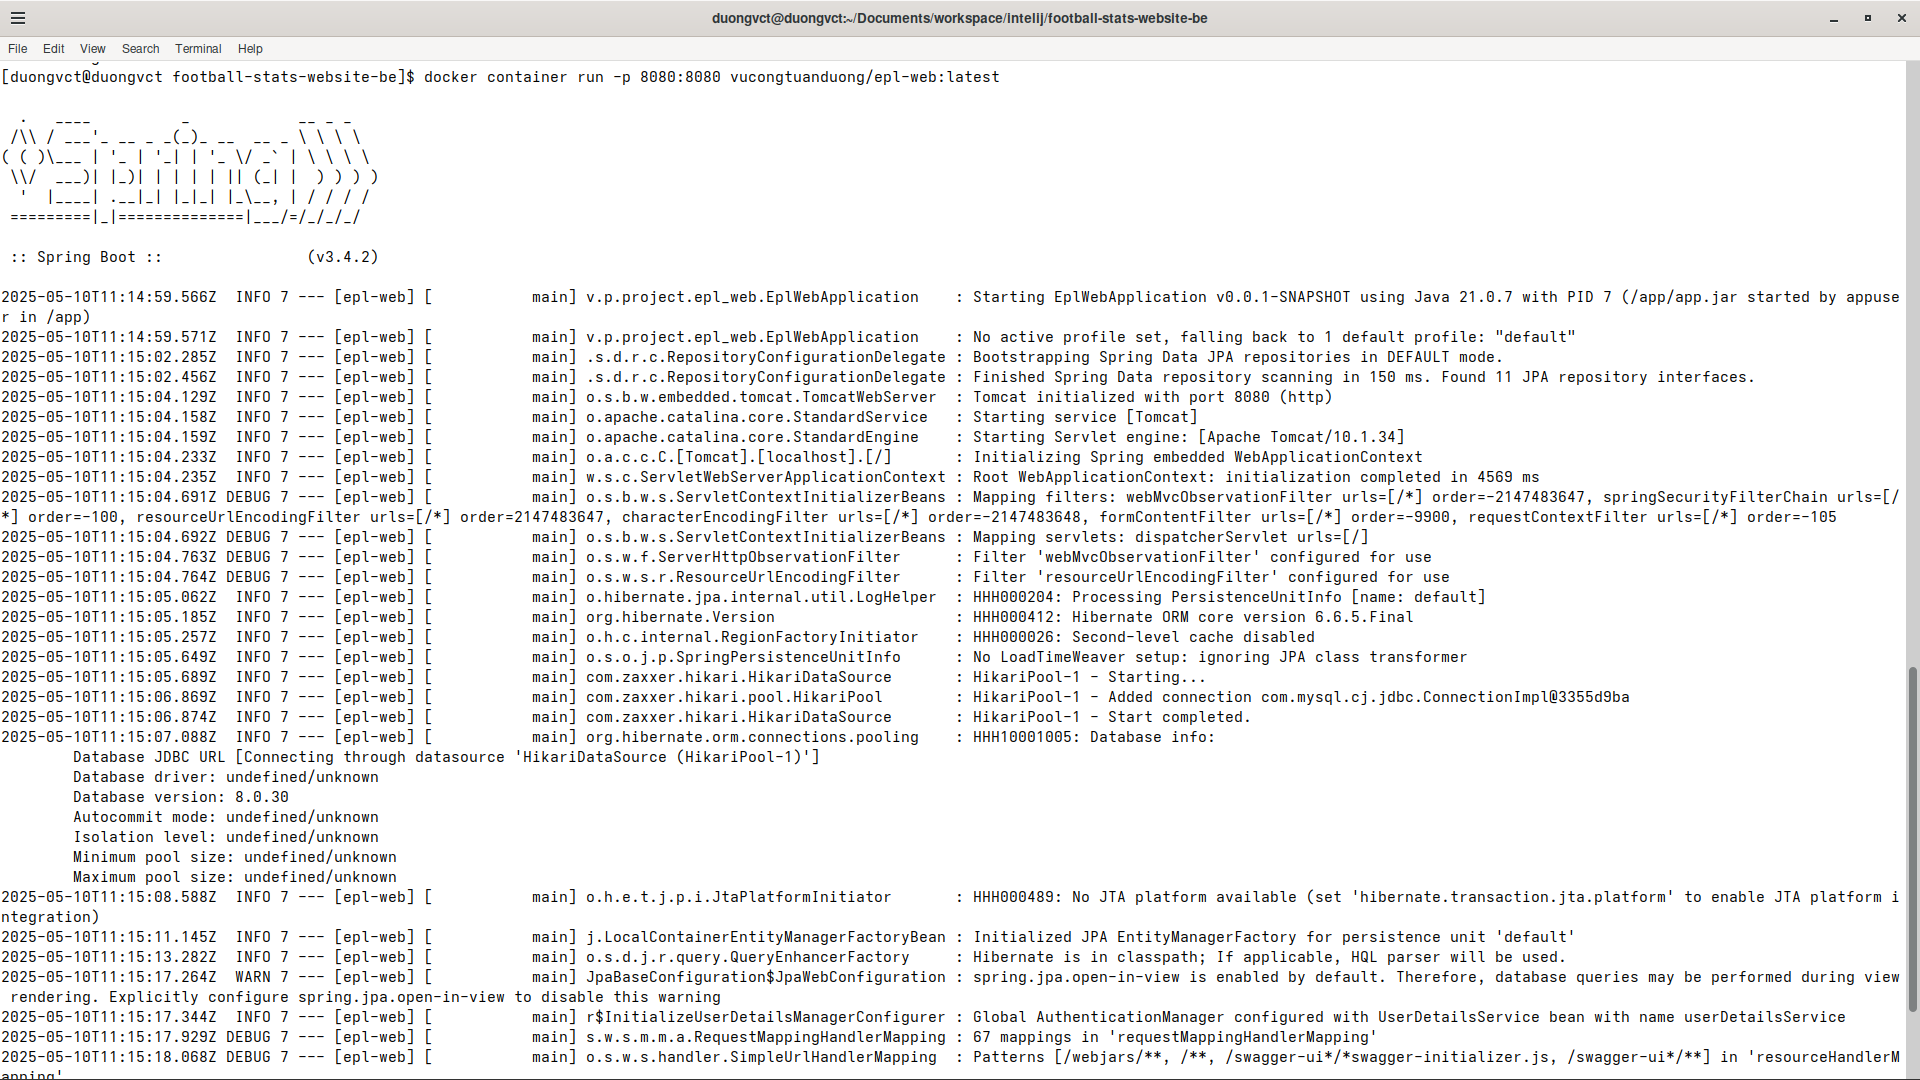
\includegraphics[width=1\linewidth]{Hinhve/docker-container-run-be1.png}
    \caption{ Kết quả chạy Docker container phía backend - ảnh 1}
    \label{fig:docker-container-run-be1}
\end{figure}
\begin{figure}
    \centering
    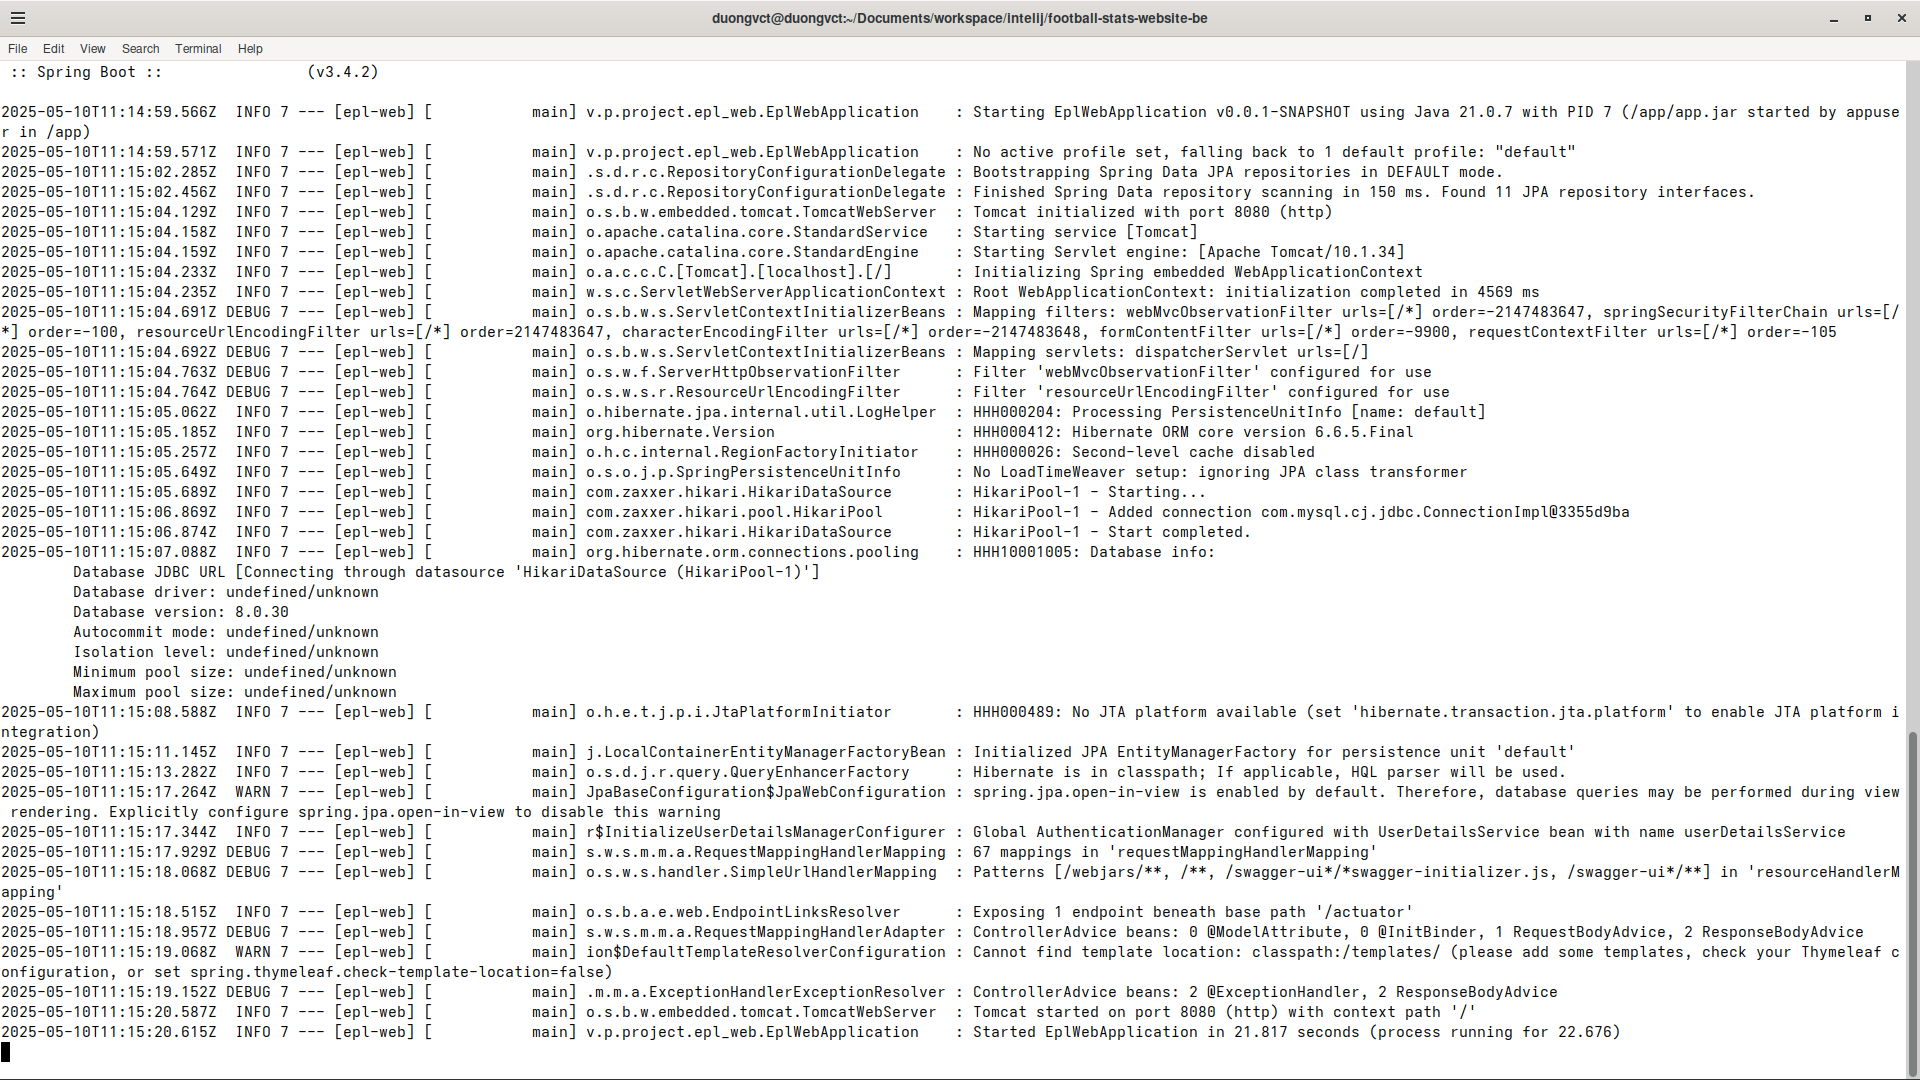
\includegraphics[width=1\linewidth]{Hinhve/docker-container-run-be2.png}
    \caption{Kết quả chạy Docker container phía backend - ảnh 2}
    \label{fig:docker-container-run-be2}
\end{figure}
\begin{figure}
    \centering
    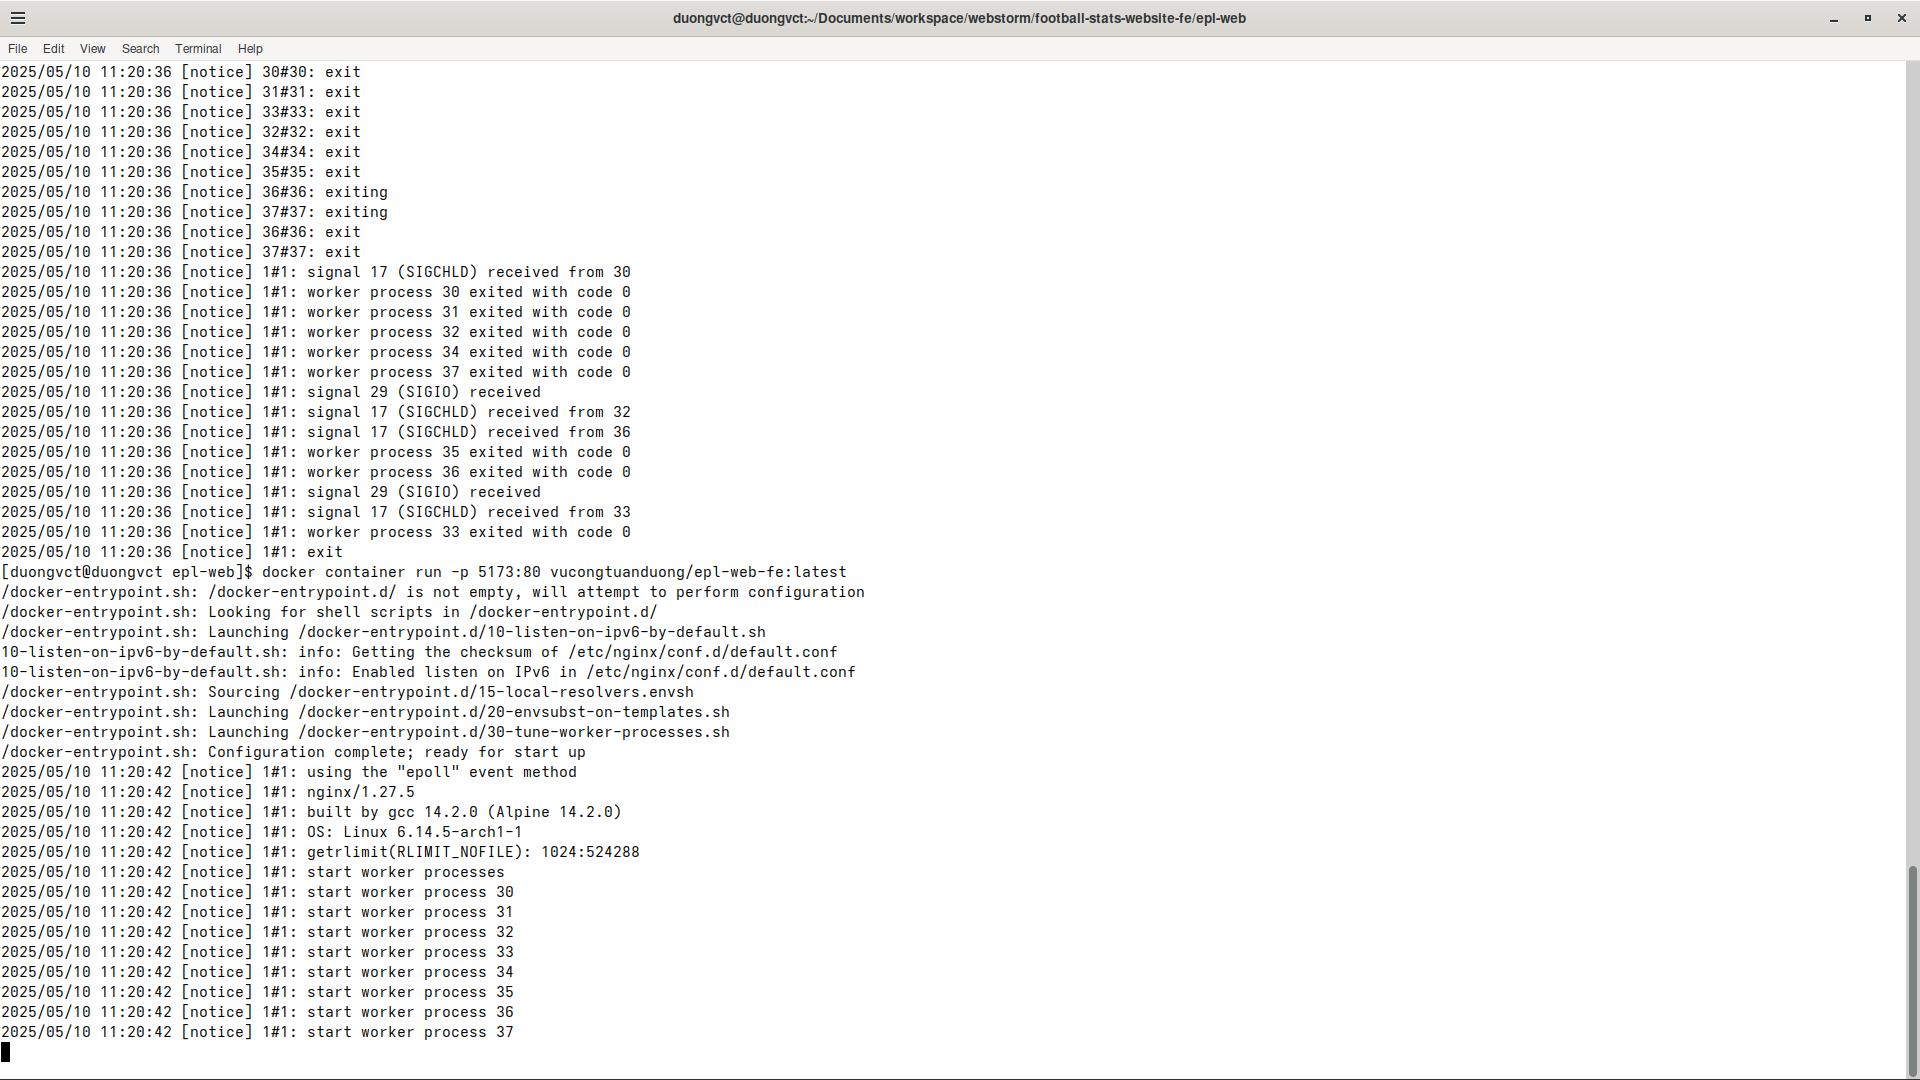
\includegraphics[width=1\linewidth]{Hinhve/docker-container-run-fe.png}
    \caption{Kết quả chạy Docker container phía frontend}
    \label{fig:docker-container-run-fe}
\end{figure}
\begin{figure}
    \centering
    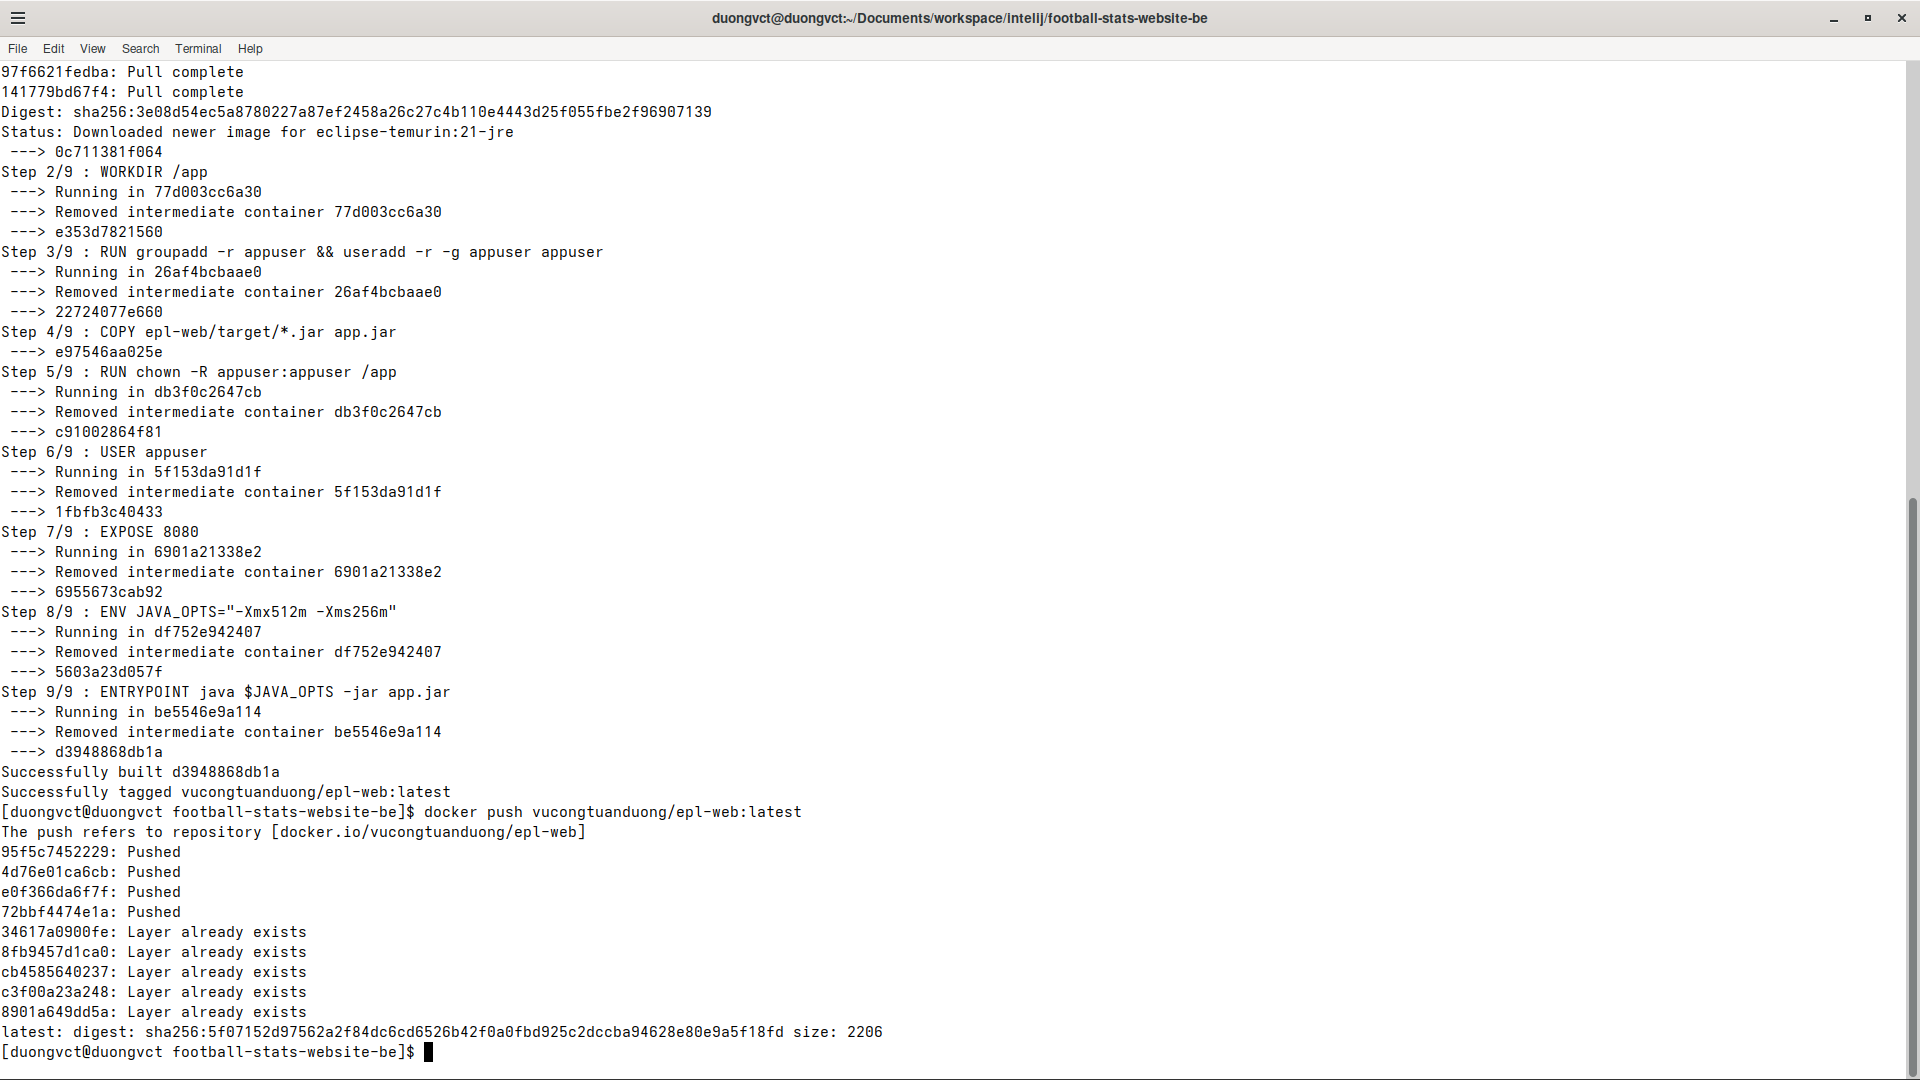
\includegraphics[width=1\linewidth]{Hinhve/docker-push-be.png}
    \caption{Kết quả chạy lệnh đẩy lên Dockerhub phía backend}
    \label{fig:docker-push-be}
\end{figure}
\begin{figure}
    \centering
    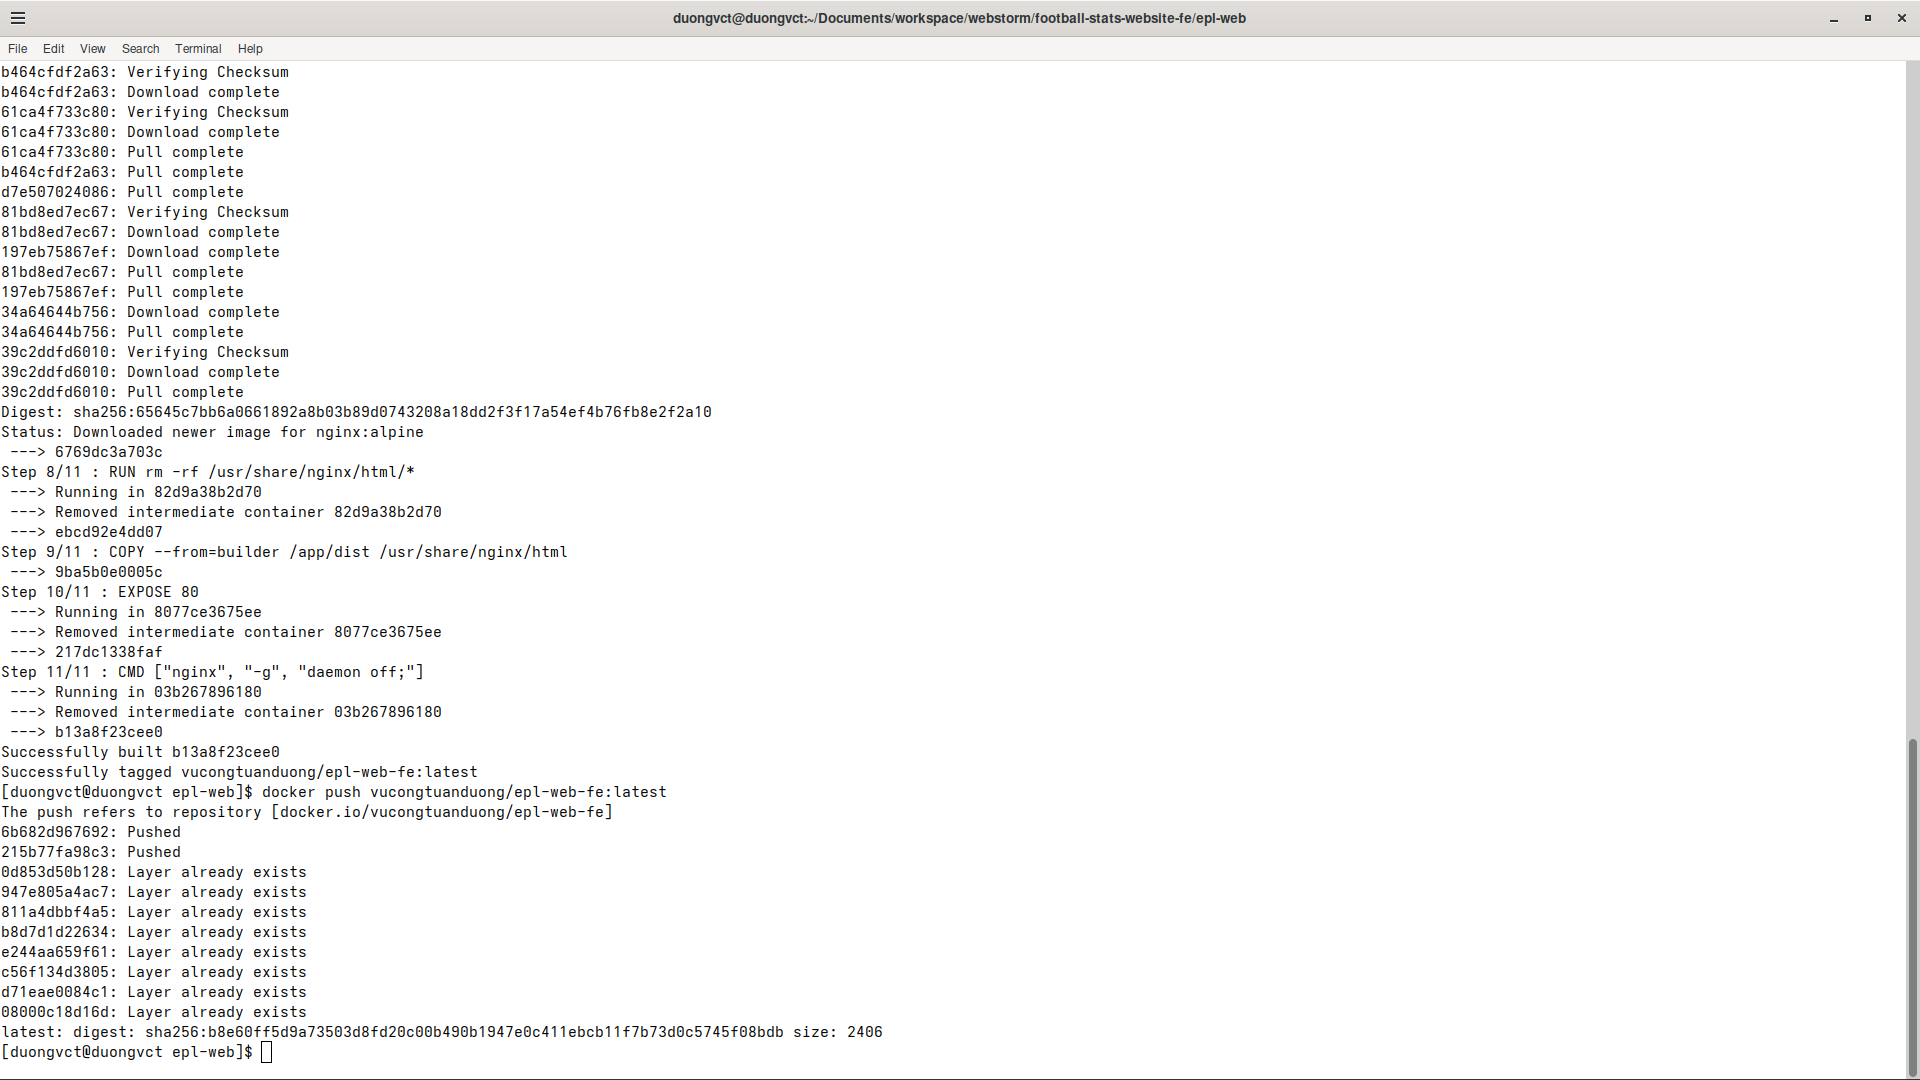
\includegraphics[width=1\linewidth]{Hinhve/docker-push-fe.png}
    \caption{Kết quả chạy lệnh đẩy lên Dockerhub phía backend}
    \label{fig:docker-push-fe}
\end{figure}
\subsection{ Cài đặt môi trường hosting ảnh - Cloudinary}
Để sử dụng Cloudinary thì ban đầu cần phải tạo tài khoản Cloudinary rồi tiến hành đăng nhập rồi sau đó vào Settings, chọn API Keys, giao diện và tên cloud như trên hình \ref{fig:cloudinary-setting}, khi đó giao diện hiển thị yêu cầu nhập mã để xác thực đã gửi trong email, như trên hình \ref{fig:cloudinary-email-verification} và phải vào email để nhận mã, như trên hình \ref{fig:cloudinary-email-code}. Sau khi nhập mã xong, một API Key mới được tạo và nhấn vào hình con mắt để đọc được và sao chép, như trên hình \ref{fig:cloudinary-api-key}, sau khi đủ thông tin thì sẽ nhập vào trong file application.properties:
\begin{verbatim}
cloudinary.cloud-name=
cloudinary.api-key=
cloudinary.api-secret=
\end{verbatim}
\begin{figure}
    \centering
    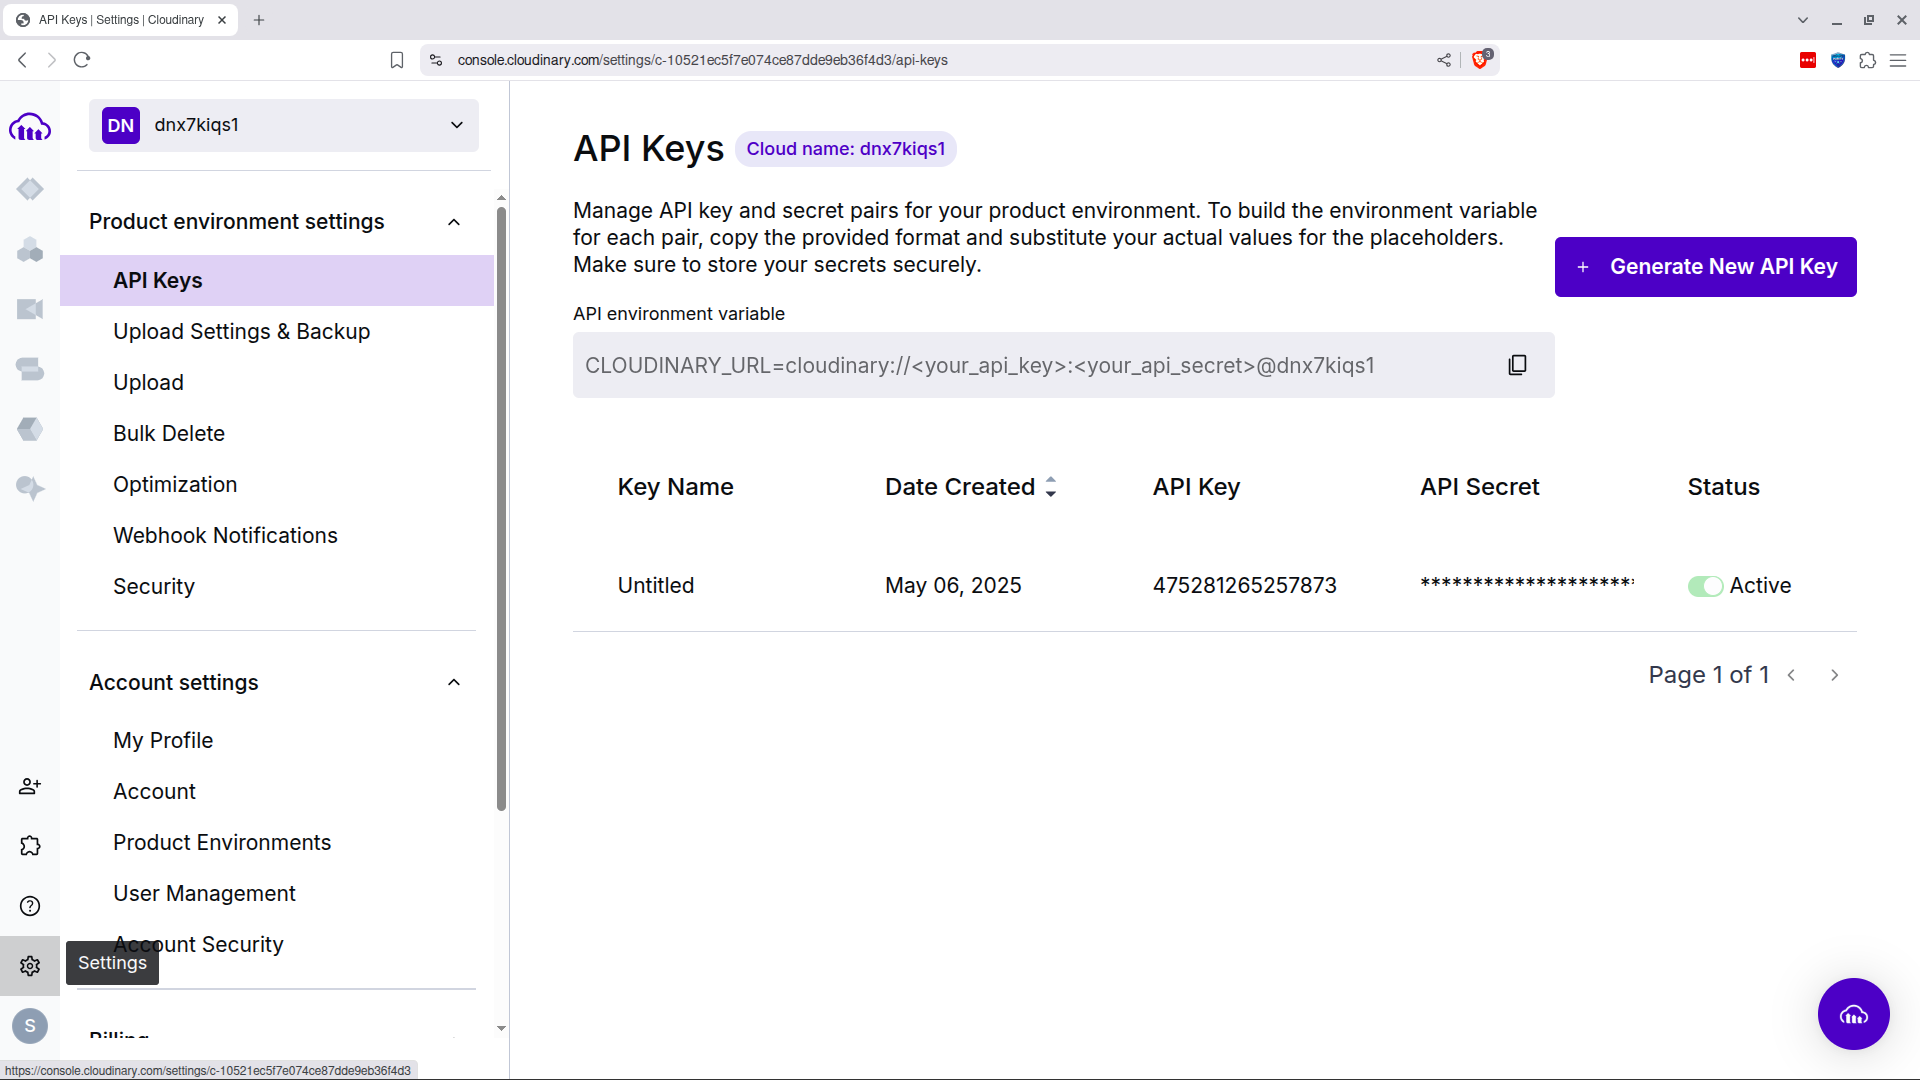
\includegraphics[width=1\linewidth]{Hinhve/cloudinary-setting.png}
    \caption{ Giao diện cài đặt và API Keys}
    \label{fig:cloudinary-setting}
\end{figure}
\begin{figure}
    \centering
    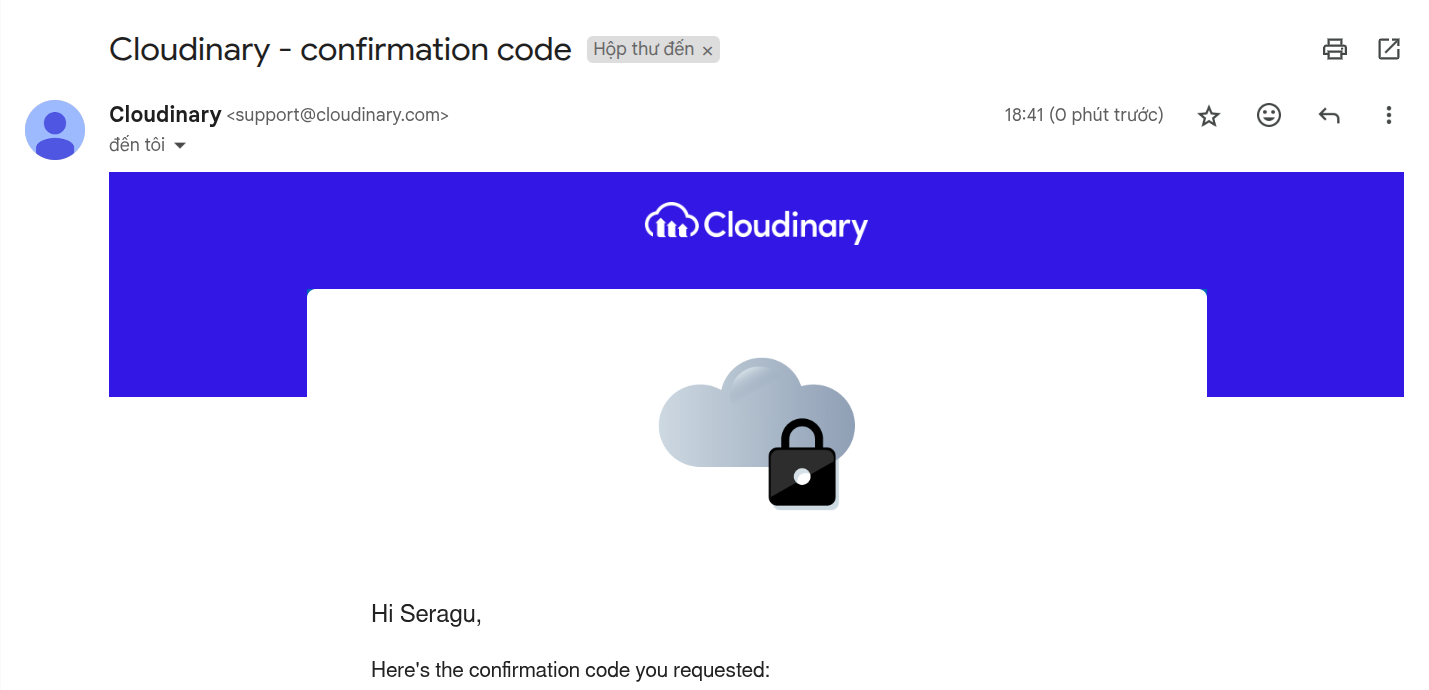
\includegraphics[width=1\linewidth]{Hinhve/cloudinary-email-code.png}
    \caption{ Email nhận mã xác thực của Cloudinary}
    \label{fig:cloudinary-email-code}
\end{figure}
\begin{figure}
    \centering
    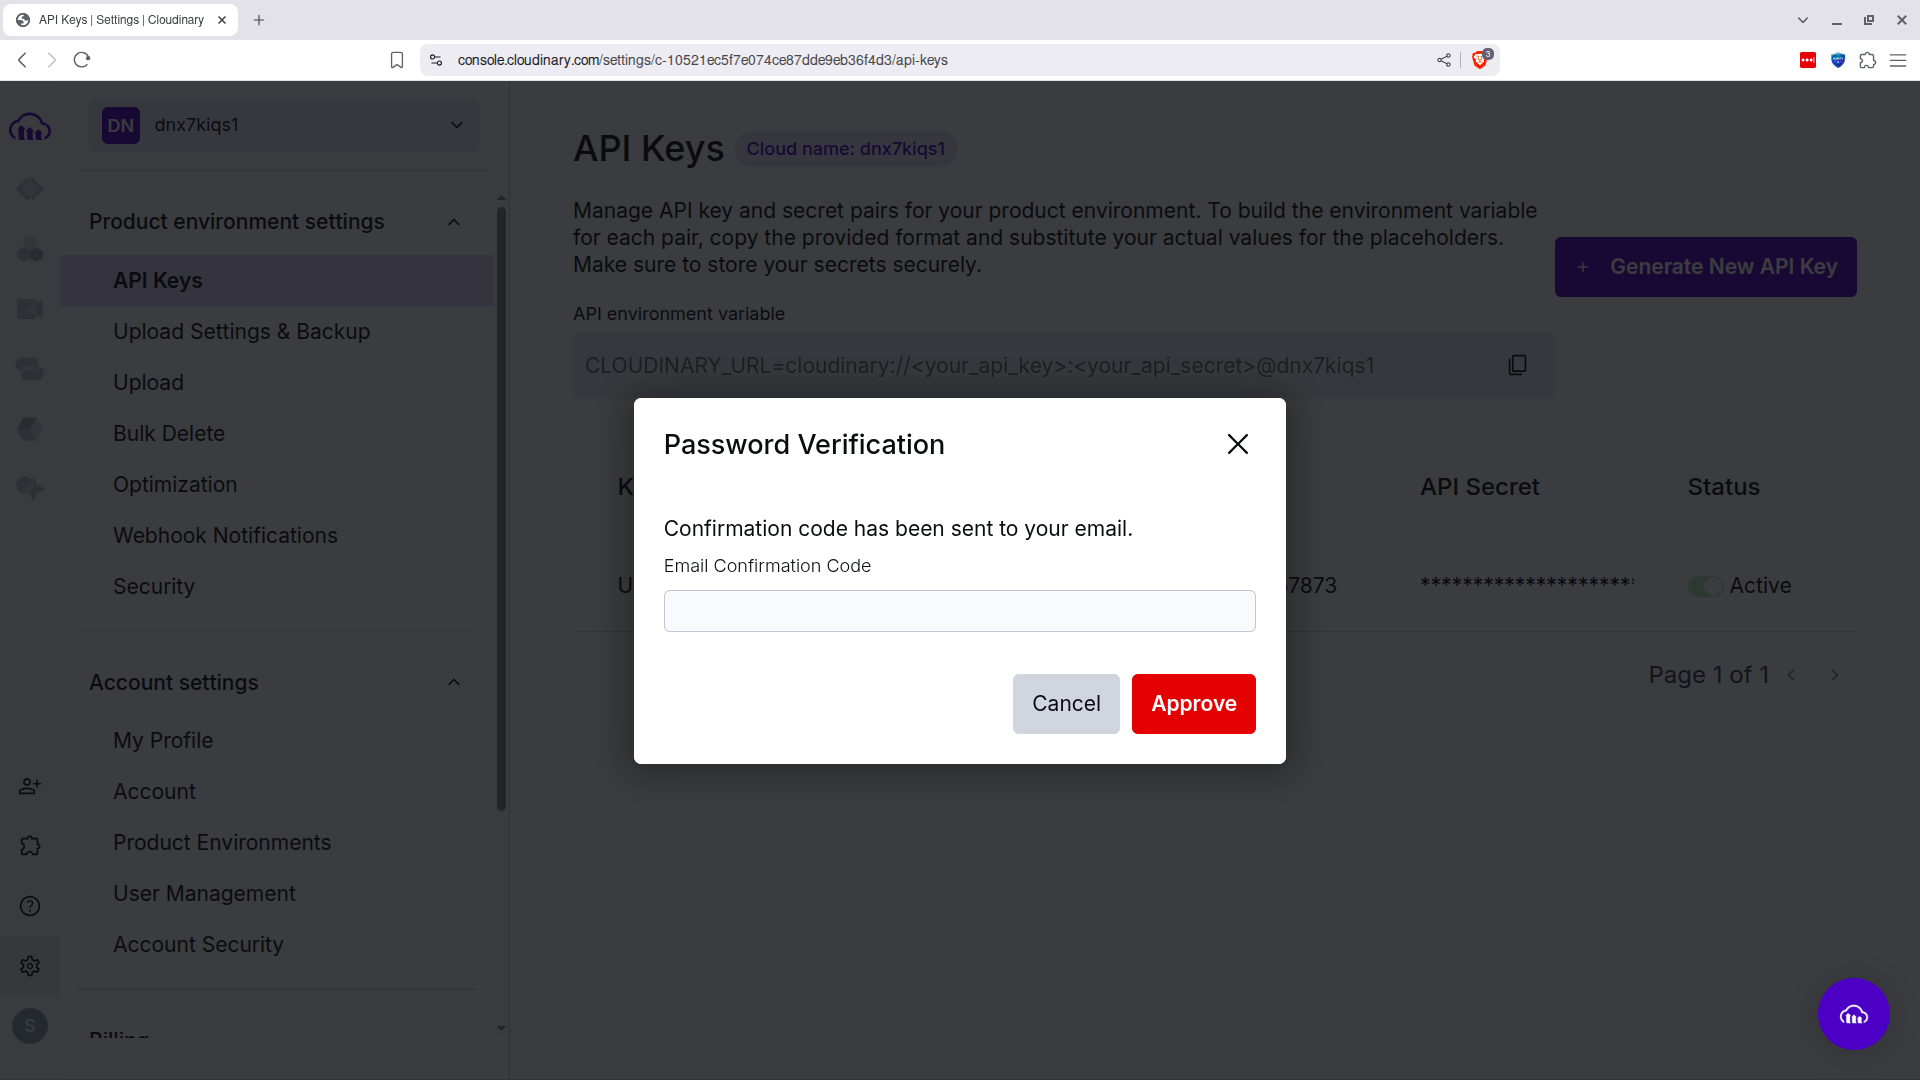
\includegraphics[width=1\linewidth]{Hinhve/cloudinary-email-verification.png}
    \caption{ Giao diện nhập mã xác thực}
    \label{fig:cloudinary-email-verification}
\end{figure}
\begin{figure}
    \centering
    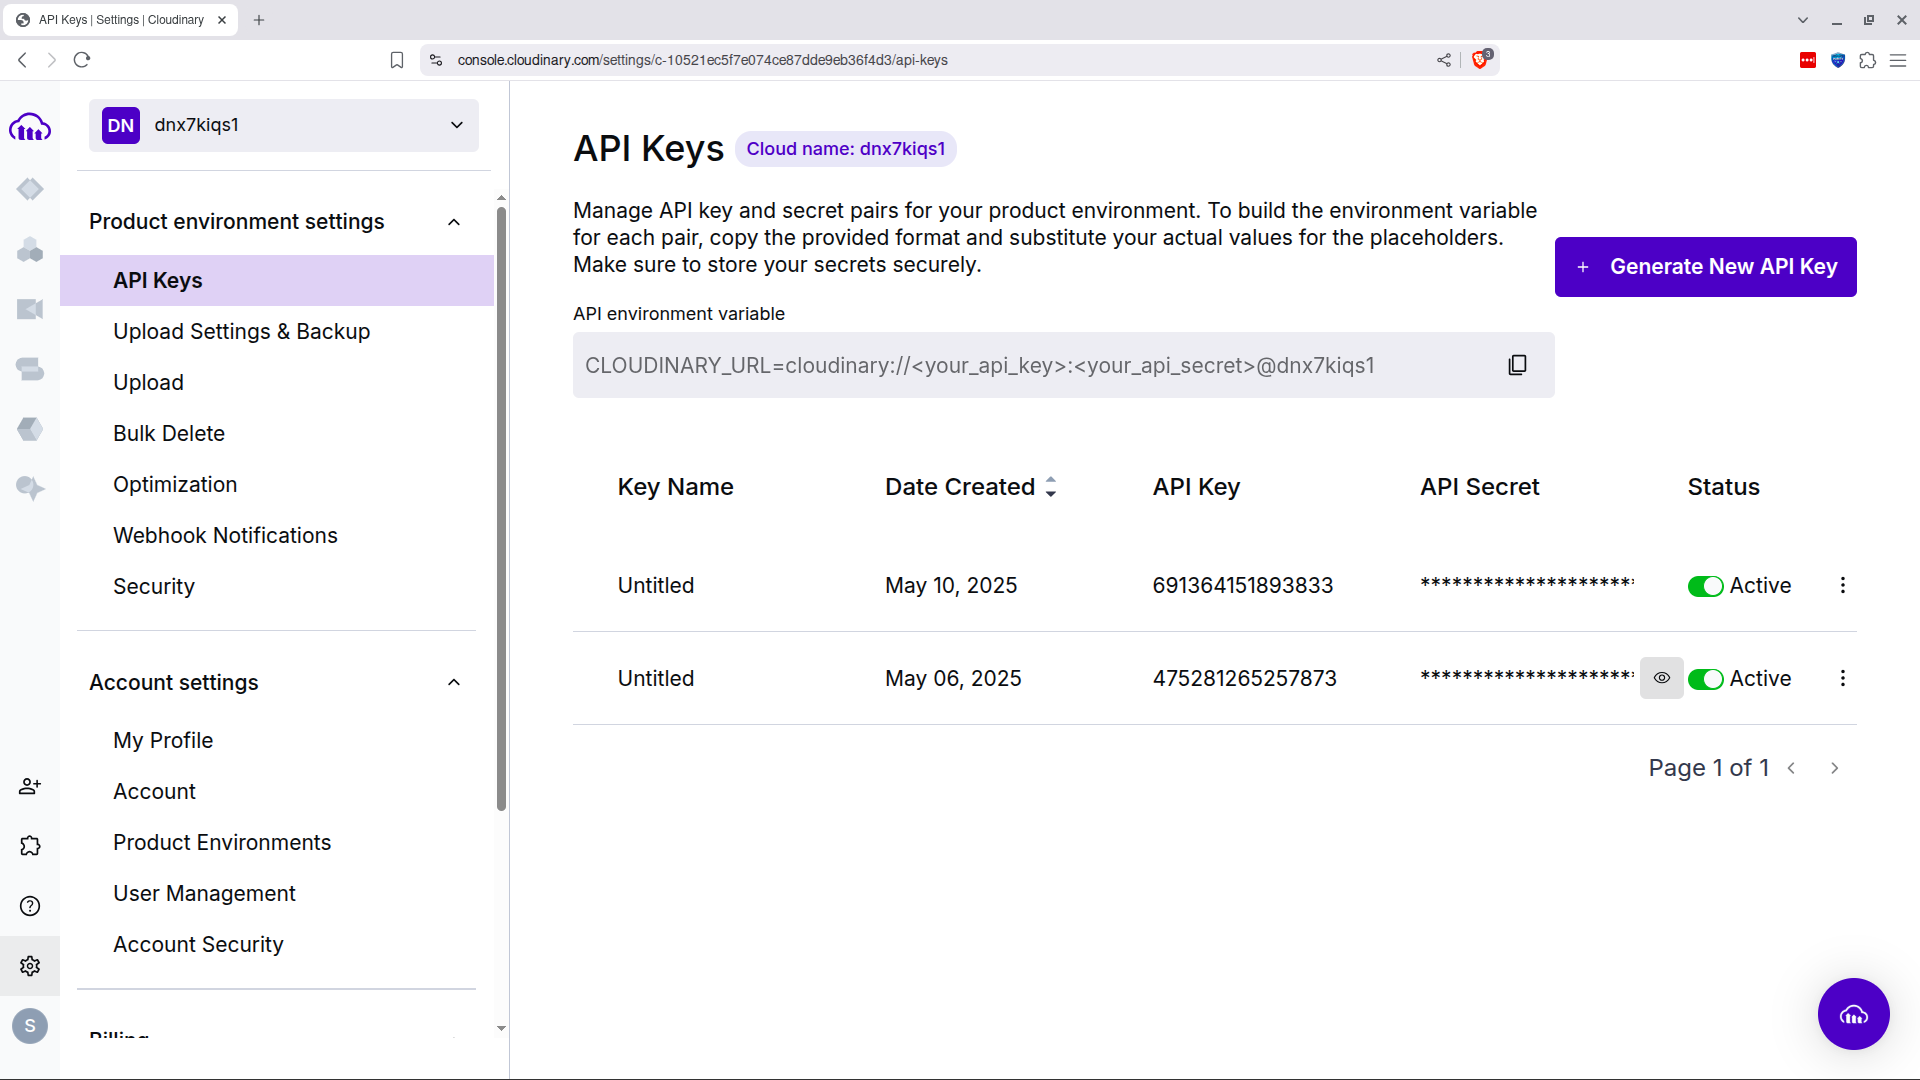
\includegraphics[width=1\linewidth]{Hinhve/cloudinary-api-key.png}
    \caption{ Giao diện API Key}
    \label{fig:cloudinary-api-key}
\end{figure}
\section{ Tài liệu API}
Chỉ có API xử lý đăng ký là không có phương thức xác thực sử dụng Bearer Token, còn tất cả các API còn lại đều có phương thức xác thực là Bearer Token và phải truyền JWT Token qua Bearer Token

Tất cả các API trả về (Responses) đều có dạng như sau:
\begin{verbatim}
{
    "statusCode": ,
    "error": ,
    "message": "",
    "data": {
        
    }
}
\end{verbatim}
\subsection{ API xử lý xác thực và phân quyền}
\subsubsection{ API xử lý đăng ký}
\begin{itemize}
    \item Phương thức: POST
    \item Endpoint: /api/v1/auth/register
    \item Request body: 
        \begin{verbatim}
{
  "email": "string",
  "name": "string",
  "password": "string"
}
        \end{verbatim}
    \item Response:
        \begin{verbatim}          
{
  "id": 9007199254740991,
  "name": "string",
  "email": "string"
}
        \end{verbatim}
\end{itemize}
\subsubsection{ API xử lý đăng xuất}
\begin{itemize}
    \item Phương thức: POST
    \item Endpoint: /api/v1/auth/logout
\end{itemize}
\subsubsection{ API xử lý đăng nhập}
\begin{itemize}
    \item Phương thức: POST
    \item Endpoint: /api/v1/auth/login
    \item Request body: 
        \begin{verbatim}
{
  "username": "string",
  "password": "string"
}
        \end{verbatim}
    \item Response:
        \begin{verbatim}          
{
  "user": {
    "id": 9007199254740991,
    "email": "string",
    "name": "string",
    "role": "string"
  },
  "access_token": "string"
}
        \end{verbatim}
\end{itemize}
\subsubsection{ API lấy Access Token mới sử dụng Refresh Token}
\begin{itemize}
    \item Phương thức: GET
    \item Endpoint: /api/v1/auth/refresh
    \item Truyền refresh token vào trong cookie
    \item Response:
        \begin{verbatim}          
{
  "user": {
    "id": 9007199254740991,
    "email": "string",
    "name": "string",
    "role": "string"
  },
  "access_token": "string"
}
        \end{verbatim}
\end{itemize}
\subsubsection{ API xử lý lấy và kiểm tra thông tin tài khoản}
\begin{itemize}
    \item Phương thức: GET
    \item Endpoint: /api/v1/auth/account
    \item Request body: 
    \item Response:
        \begin{verbatim}          
{
  "user": {
    "id": 9007199254740991,
    "email": "string",
    "name": "string",
    "role": "string"
  }
}
        \end{verbatim}
\end{itemize}
\subsection{ API chuyển nhượng}
\subsubsection{ Sửa chuyển nhượng}
\begin{itemize}
    \item Phương thức: PUT
    \item Endpoint: /api/v1/transfers
    \item Request body: 
        \begin{verbatim}
{
  "id": 9007199254740991,
  "date": "2025-05-09",
  "type": "string",
  "playerValue": 0.1,
  "fee": 0.1,
  "player": 9007199254740991,
  "club": 9007199254740991
}
        \end{verbatim}
    \item Response:
        \begin{verbatim}          
{
  "id": 9007199254740991,
  "date": "2025-05-09",
  "type": "string",
  "playerValue": 0.1,
  "fee": 0.1,
  "player": "string",
  "club": "string",
  "previousClub": "string"
}
        \end{verbatim}
\end{itemize}
\subsubsection{ Tạo chuyển nhượng}
\begin{itemize}
    \item Phương thức: POST
    \item Endpoint: /api/v1/transfers
    \item Request body: 
        \begin{verbatim}
{
  "date": "2025-05-09",
  "type": "string",
  "playerValue": 0.1,
  "fee": 0.1,
  "player": 9007199254740991,
  "club": 9007199254740991
}
        \end{verbatim}
    \item Response:
        \begin{verbatim}          
{
  "id": 9007199254740991,
  "date": "2025-05-09",
  "type": "string",
  "playerValue": 0.1,
  "fee": 0.1,
  "player": "string",
  "club": "string",
  "previousClub": "string"
}
        \end{verbatim}
\end{itemize}
\subsubsection{ Xóa chuyển nhượng}
\begin{itemize}
    \item Phương thức: DELETE
    \item Endpoint: /api/v1/transfers/{id}
    \item {id} là id của chuyển nhượng muốn xóa
\end{itemize}
\subsection{ API cầu thủ}
\subsubsection{ Lấy danh sách cầu thủ có phân trang}
\begin{itemize}
    \item Phương thức: GET
    \item Endpoint: /api/v1/players?page={page}\&size={size}\&filter={filter}
    \item {page} là số trang, {size} là số cầu thủ mỗi trang, {filter} là tiêu chí để tìm kiếm
    \item Response:
        \begin{verbatim}          
{
  "meta": {
    "page": 1073741824,
    "pageSize": 1073741824,
    "pages": 1073741824,
    "total": 9007199254740991
  },
  "result": {}
}
        \end{verbatim}
\end{itemize}
\subsubsection{ Sửa cầu thủ}
\begin{itemize}
    \item Phương thức: PUT
    \item Endpoint: /api/v1/players
    \item Request body: 
        \begin{verbatim}
{
  "id": 9007199254740991,
  "name": "string",
  "dob": "2025-05-09",
  "shirtNumber": 1073741824,
  "marketValue": 0.1,
  "citizenships": [
    "string"
  ],
  "positions": [
    "string"
  ],
  "imageUrl": "string"
}
        \end{verbatim}
    \item Response:
        \begin{verbatim}          
{
  "id": 9007199254740991,
  "name": "string",
  "age": 1073741824,
  "dob": "2025-05-09",
  "shirtNumber": 1073741824,
  "marketValue": 0.1,
  "citizenships": [
    "string"
  ],
  "positions": [
    "string"
  ],
  "transferHistories": [
    {
      "id": 9007199254740991,
      "date": "2025-05-09",
      "type": "string",
      "playerValue": 0.1,
      "fee": 0.1,
      "player": "string",
      "club": "string",
      "previousClub": "string"
    }
  ],
  "imageUrl": "string"
}
        \end{verbatim}
\end{itemize}
\subsubsection{ Tạo cầu thủ}
\begin{itemize}
    \item Phương thức: POST
    \item Endpoint: /api/v1/players
    \item Request body: 
        \begin{verbatim}
{
  "name": "string",
  "dob": "2025-05-09",
  "shirtNumber": 1073741824,
  "marketValue": 0.1,
  "citizenships": [
    "string"
  ],
  "positions": [
    "string"
  ],
  "imageUrl": "string"
}
        \end{verbatim}
    \item Response:
        \begin{verbatim}          
{
  "id": 9007199254740991,
  "name": "string",
  "age": 1073741824,
  "dob": "2025-05-09",
  "shirtNumber": 1073741824,
  "marketValue": 0.1,
  "citizenships": [
    "string"
  ],
  "positions": [
    "string"
  ],
  "imageUrl": "string"
}
        \end{verbatim}
\end{itemize}
\subsubsection{ Lấy 1 cầu thủ cụ thể}
\begin{itemize}
    \item Phương thức: GET
    \item Endpoint: /api/v1/players/{id}?sortTransferHistory=false
    \item {id} là id cầu thủ, có thể có 1 tham số tùy chọn sortTransferHistory để sắp xếp lịch sử chuyển nhượng theo thứ tự gần nhất
    \item Response:
        \begin{verbatim}          
{
  "id": 9007199254740991,
  "name": "string",
  "age": 1073741824,
  "dob": "2025-05-09",
  "shirtNumber": 1073741824,
  "marketValue": 0.1,
  "currentClub": "string",
  "citizenships": [
    "string"
  ],
  "positions": [
    "string"
  ],
  "transferHistories": [
    {
      "id": 9007199254740991,
      "date": "2025-05-09",
      "type": "string",
      "playerValue": 0.1,
      "fee": 0.1,
      "player": "string",
      "club": "string",
      "previousClub": "string"
    }
  ],
  "imageUrl": "string"
}
        \end{verbatim}
\end{itemize}
\subsubsection{ Xóa cầu thủ}
\begin{itemize}
    \item Phương thức: DELETE
    \item Endpoint: /api/v1/players/{id}
    \item {id} là id cầu thủ
\end{itemize}
\subsection{ API xử lý trận đấu}
\subsubsection{ Lấy thông tin tất cả trận đấu có phân trang}
\begin{itemize}
    \item Phương thức: GET
    \item Endpoint: /api/v1/matches?page={page}\&size={size}\&filter={filter}
    \item {page} là số trang, {size} là số cầu thủ mỗi trang, {filter} là tiêu chí để tìm kiếm
    \item Response:
        \begin{verbatim}          
{
  "meta": {
    "page": 1073741824,
    "pageSize": 1073741824,
    "pages": 1073741824,
    "total": 9007199254740991
  },
  "result": {}
}
        \end{verbatim}
\end{itemize}
\subsubsection{ Sửa trận đấu}
\begin{itemize}
    \item Phương thức: PUT
    \item Endpoint: /api/v1/matches
    \item Request body: 
        \begin{verbatim}
{
  "id": 9007199254740991,
  "host": 9007199254740991,
  "away": 9007199254740991,
  "season": 9007199254740991,
  "round": 1073741824,
  "awayScore": 1073741824,
  "hostScore": 1073741824,
  "date": "2025-05-09T10:57:39.062Z"
}
        \end{verbatim}
    \item Response:
        \begin{verbatim}
{
  "id": 9007199254740991,
  "host": {
    "id": 9007199254740991,
    "name": "string",
    "country": "string",
    "stadiumName": "string",
    "transferHistories": [
      {
        "id": 9007199254740991,
        "date": "2025-05-09",
        "type": "string",
        "playerValue": 0.1,
        "fee": 0.1,
        "player": "string",
        "club": "string",
        "previousClub": "string"
      }
    ],
    "currentCoach": {
      "id": 9007199254740991,
      "name": "string",
      "dob": "2025-05-09",
      "citizenships": [
        "string"
      ]
    },
    "currentPlayerList": [
      {
        "id": 9007199254740991,
        "name": "string",
        "dob": "2025-05-09",
        "shirtNumber": 1073741824,
        "marketValue": 0.1,
        "citizenships": [
          "string"
        ],
        "positions": [
          "string"
        ]
      }
    ],
    "imageUrl": "string"
  },
  "away": {
    "id": 9007199254740991,
    "name": "string",
    "country": "string",
    "stadiumName": "string",
    "transferHistories": [
      {
        "id": 9007199254740991,
        "date": "2025-05-09",
        "type": "string",
        "playerValue": 0.1,
        "fee": 0.1,
        "player": "string",
        "club": "string",
        "previousClub": "string"
      }
    ],
    "currentCoach": {
      "id": 9007199254740991,
      "name": "string",
      "dob": "2025-05-09",
      "citizenships": [
        "string"
      ]
    },
    "currentPlayerList": [
      {
        "id": 9007199254740991,
        "name": "string",
        "dob": "2025-05-09",
        "shirtNumber": 1073741824,
        "marketValue": 0.1,
        "citizenships": [
          "string"
        ],
        "positions": [
          "string"
        ]
      }
    ],
    "imageUrl": "string"
  },
  "season": {
    "id": 9007199254740991,
    "name": "string",
    "startDate": "2025-05-09",
    "endDate": "2025-05-09"
  },
  "round": 1073741824,
  "awayScore": 1073741824,
  "hostScore": 1073741824,
  "date": "2025-05-09T10:57:39.065Z",
  "matchActions": [
    {
      "id": 9007199254740991,
      "action": "string",
      "minute": 1073741824,
      "player": {
        "id": 9007199254740991,
        "name": "string",
        "age": 1073741824,
        "dob": "2025-05-09",
        "shirtNumber": 1073741824,
        "marketValue": 0.1,
        "currentClub": "string",
        "citizenships": [
          "string"
        ],
        "positions": [
          "string"
        ],
        "transferHistories": [
          {
            "id": 9007199254740991,
            "date": "2025-05-09",
            "type": "string",
            "playerValue": 0.1,
            "fee": 0.1,
            "player": "string",
            "club": "string",
            "previousClub": "string"
          }
        ],
        "imageUrl": "string"
      }
    }
  ]
}
        \end{verbatim}
\end{itemize}

\subsubsection{ Tạo trận đấu}
\begin{itemize}
    \item Phương thức: POST
    \item Endpoint: /api/v1/matches
    \item Request body: 
        \begin{verbatim}
{
  "host": 9007199254740991,
  "away": 9007199254740991,
  "season": 9007199254740991,
  "round": 1073741824,
  "awayScore": 1073741824,
  "hostScore": 1073741824,
  "date": "2025-05-09T10:59:59.350Z"
}
        \end{verbatim}
    \item Response:
        \begin{verbatim}
{
  "id": 9007199254740991,
  "host": {
    "id": 9007199254740991,
    "name": "string",
    "country": "string",
    "stadiumName": "string",
    "transferHistories": [
      {
        "id": 9007199254740991,
        "date": "2025-05-09",
        "type": "string",
        "playerValue": 0.1,
        "fee": 0.1,
        "player": "string",
        "club": "string",
        "previousClub": "string"
      }
    ],
    "currentCoach": {
      "id": 9007199254740991,
      "name": "string",
      "dob": "2025-05-09",
      "citizenships": [
        "string"
      ]
    },
    "currentPlayerList": [
      {
        "id": 9007199254740991,
        "name": "string",
        "dob": "2025-05-09",
        "shirtNumber": 1073741824,
        "marketValue": 0.1,
        "citizenships": [
          "string"
        ],
        "positions": [
          "string"
        ]
      }
    ],
    "imageUrl": "string"
  },
  "away": {
    "id": 9007199254740991,
    "name": "string",
    "country": "string",
    "stadiumName": "string",
    "transferHistories": [
      {
        "id": 9007199254740991,
        "date": "2025-05-09",
        "type": "string",
        "playerValue": 0.1,
        "fee": 0.1,
        "player": "string",
        "club": "string",
        "previousClub": "string"
      }
    ],
    "currentCoach": {
      "id": 9007199254740991,
      "name": "string",
      "dob": "2025-05-09",
      "citizenships": [
        "string"
      ]
    },
    "currentPlayerList": [
      {
        "id": 9007199254740991,
        "name": "string",
        "dob": "2025-05-09",
        "shirtNumber": 1073741824,
        "marketValue": 0.1,
        "citizenships": [
          "string"
        ],
        "positions": [
          "string"
        ]
      }
    ],
    "imageUrl": "string"
  },
  "season": {
    "id": 9007199254740991,
    "name": "string",
    "startDate": "2025-05-09",
    "endDate": "2025-05-09"
  },
  "round": 1073741824,
  "awayScore": 1073741824,
  "hostScore": 1073741824,
  "date": "2025-05-09T10:59:59.352Z"
}
        \end{verbatim}
\end{itemize}

\subsubsection{ Lấy 1 trận đấu cụ thể}
\begin{itemize}
    \item Phương thức: GET
    \item Endpoint: /api/v1/matches/{id}
    \item {id} là id trận đấu
    \item Response:
        \begin{verbatim}
{
  "id": 9007199254740991,
  "host": {
    "id": 9007199254740991,
    "name": "string",
    "country": "string",
    "stadiumName": "string",
    "transferHistories": [
      {
        "id": 9007199254740991,
        "date": "2025-05-09",
        "type": "string",
        "playerValue": 0.1,
        "fee": 0.1,
        "player": "string",
        "club": "string",
        "previousClub": "string"
      }
    ],
    "currentCoach": {
      "id": 9007199254740991,
      "name": "string",
      "dob": "2025-05-09",
      "citizenships": [
        "string"
      ]
    },
    "currentPlayerList": [
      {
        "id": 9007199254740991,
        "name": "string",
        "dob": "2025-05-09",
        "shirtNumber": 1073741824,
        "marketValue": 0.1,
        "citizenships": [
          "string"
        ],
        "positions": [
          "string"
        ]
      }
    ],
    "imageUrl": "string"
  },
  "away": {
    "id": 9007199254740991,
    "name": "string",
    "country": "string",
    "stadiumName": "string",
    "transferHistories": [
      {
        "id": 9007199254740991,
        "date": "2025-05-09",
        "type": "string",
        "playerValue": 0.1,
        "fee": 0.1,
        "player": "string",
        "club": "string",
        "previousClub": "string"
      }
    ],
    "currentCoach": {
      "id": 9007199254740991,
      "name": "string",
      "dob": "2025-05-09",
      "citizenships": [
        "string"
      ]
    },
    "currentPlayerList": [
      {
        "id": 9007199254740991,
        "name": "string",
        "dob": "2025-05-09",
        "shirtNumber": 1073741824,
        "marketValue": 0.1,
        "citizenships": [
          "string"
        ],
        "positions": [
          "string"
        ]
      }
    ],
    "imageUrl": "string"
  },
  "season": {
    "id": 9007199254740991,
    "name": "string",
    "startDate": "2025-05-09",
    "endDate": "2025-05-09"
  },
  "round": 1073741824,
  "awayScore": 1073741824,
  "hostScore": 1073741824,
  "date": "2025-05-09T11:07:44.468Z",
  "matchActions": [
    {
      "id": 9007199254740991,
      "action": "string",
      "minute": 1073741824,
      "player": {
        "id": 9007199254740991,
        "name": "string",
        "age": 1073741824,
        "dob": "2025-05-09",
        "shirtNumber": 1073741824,
        "marketValue": 0.1,
        "currentClub": "string",
        "citizenships": [
          "string"
        ],
        "positions": [
          "string"
        ],
        "transferHistories": [
          {
            "id": 9007199254740991,
            "date": "2025-05-09",
            "type": "string",
            "playerValue": 0.1,
            "fee": 0.1,
            "player": "string",
            "club": "string",
            "previousClub": "string"
          }
        ],
        "imageUrl": "string"
      }
    }
  ]
}
        \end{verbatim}
\end{itemize}

\subsubsection{ Xóa trận đấu}
\begin{itemize}
    \item Phương thức: DELETE
    \item Endpoint: /api/v1/matches/{id}
    \item {id} là id trận đấu
\end{itemize}

\subsection{ API hành động trong trận đấu}
\subsubsection{ Lấy tất cả các hành động trong trận đấu có phân trang}
\begin{itemize}
    \item Phương thức: GET
    \item Endpoint: /api/v1/match-actions?page={page}\&size={size}\&filter={filter}
    \item {page} là số trang, {size} là số cầu thủ mỗi trang, {filter} là tiêu chí để tìm kiếm
    \item Response:
        \begin{verbatim}
{
  "meta": {
    "page": 1073741824,
    "pageSize": 1073741824,
    "pages": 1073741824,
    "total": 9007199254740991
  },
  "result": {}
}
        \end{verbatim}
\end{itemize}

\subsubsection{ Sửa hành động trận đấu}
\begin{itemize}
    \item Phương thức: PUT
    \item Endpoint: /api/v1/match-actions
    \item Request body: 
        \begin{verbatim}
{
  "id": 9007199254740991,
  "action": "string",
  "minute": 1073741824,
  "match": 9007199254740991,
  "player": 9007199254740991
}
        \end{verbatim}
    \item Response:
        \begin{verbatim}
{
  "id": 9007199254740991,
  "action": "string",
  "minute": 1073741824,
  "match": 9007199254740991,
  "player": {
    "id": 9007199254740991,
    "name": "string",
    "age": 1073741824,
    "dob": "2025-05-09",
    "shirtNumber": 1073741824,
    "marketValue": 0.1,
    "currentClub": "string",
    "citizenships": [
      "string"
    ],
    "positions": [
      "string"
    ],
    "transferHistories": [
      {
        "id": 9007199254740991,
        "date": "2025-05-09",
        "type": "string",
        "playerValue": 0.1,
        "fee": 0.1,
        "player": "string",
        "club": "string",
        "previousClub": "string"
      }
    ],
    "imageUrl": "string"
  }
}
        \end{verbatim}
\end{itemize}

\subsubsection{ Tạo hành động trong trận đấu}
\begin{itemize}
    \item Phương thức: POST
    \item Endpoint: /api/v1/match-actions
    \item Request body: 
        \begin{verbatim}
{
  "action": "string",
  "minute": 1073741824,
  "match": 9007199254740991,
  "player": 9007199254740991
}
        \end{verbatim}
    \item Response:
        \begin{verbatim}
{
  "id": 9007199254740991,
  "action": "string",
  "minute": 1073741824,
  "match": 9007199254740991,
  "player": 9007199254740991
}
        \end{verbatim}
\end{itemize}

\subsubsection{ Lấy 1 hành động trận đấu cụ thể}
\begin{itemize}
    \item Phương thức: GET
    \item Endpoint: /api/v1/match-actions/{id}
    \item {id} là id hành động trận đấu
    \item Response:
        \begin{verbatim}
{
  "id": 9007199254740991,
  "action": "string",
  "minute": 1073741824,
  "match": 9007199254740991,
  "player": {
    "id": 9007199254740991,
    "name": "string",
    "age": 1073741824,
    "dob": "2025-05-09",
    "shirtNumber": 1073741824,
    "marketValue": 0.1,
    "currentClub": "string",
    "citizenships": [
      "string"
    ],
    "positions": [
      "string"
    ],
    "transferHistories": [
      {
        "id": 9007199254740991,
        "date": "2025-05-09",
        "type": "string",
        "playerValue": 0.1,
        "fee": 0.1,
        "player": "string",
        "club": "string",
        "previousClub": "string"
      }
    ],
    "imageUrl": "string"
  }
}
        \end{verbatim}
\end{itemize}

\subsubsection{ Xóa hành động trận đấu}
\begin{itemize}
    \item Phương thức: DELETE
    \item Endpoint: /api/v1/match-actions/{id}
    \item {id} là id hành động trận đấu
\end{itemize}

\subsection{ API giải đấu}
\subsubsection{ Lấy danh sách giải đấu có phân trang}
\begin{itemize}
    \item Phương thức: GET
    \item Endpoint: /api/v1/leagues?page={page}\&size={size}\&filter={filter}
    \item {page} là số trang, {size} là số cầu thủ mỗi trang, {filter} là tiêu chí để tìm kiếm
    \item Response:
        \begin{verbatim}
{
  "meta": {
    "page": 1073741824,
    "pageSize": 1073741824,
    "pages": 1073741824,
    "total": 9007199254740991
  },
  "result": {}
}
        \end{verbatim}
\end{itemize}

\subsubsection{ Sửa giải đấu}
\begin{itemize}
    \item Phương thức: PUT
    \item Endpoint: /api/v1/leagues
    \item Request body:
        \begin{verbatim}
{
  "id": 9007199254740991,
  "name": "string",
  "imageUrl": "string"
}
        \end{verbatim}
    \item Response:
        \begin{verbatim}
{
  "id": 9007199254740991,
  "name": "string",
  "leagueSeasons": [
    {
      "id": 9007199254740991,
      "name": "string",
      "startDate": "2025-05-09",
      "endDate": "2025-05-09"
    }
  ],
  "imageUrl": "string"
}
        \end{verbatim}
\end{itemize}

\subsubsection{ Tạo giải đấu}
\begin{itemize}
    \item Phương thức: POST
    \item Endpoint: /api/v1/leagues
    \item Request body:
        \begin{verbatim}
{
  "name": "string",
  "imageUrl": "string"
}
        \end{verbatim}
    \item Response:
        \begin{verbatim}
{
  "id": 9007199254740991,
  "name": "string",
  "imageUrl": "string"
}
        \end{verbatim}
\end{itemize}

\subsubsection{ Lấy 1 giải đấu cụ thể}
\begin{itemize}
    \item Phương thức: GET
    \item Endpoint: /api/v1/leagues/{id}
    \item {id} là id giải đấu
    \item Response:
        \begin{verbatim}
{
  "id": 9007199254740991,
  "name": "string",
  "leagueSeasons": [
    {
      "id": 9007199254740991,
      "name": "string",
      "startDate": "2025-05-09",
      "endDate": "2025-05-09"
    }
  ],
  "imageUrl": "string"
}
        \end{verbatim}
\end{itemize}

\subsubsection{ Xóa giải đấu}
\begin{itemize}
    \item Phương thức: DELETE
    \item Endpoint: /api/v1/leagues/{id}
    \item {id} là id giải đấu
\end{itemize}

\subsubsection{ Lấy danh sách câu lạc bộ thắng nhiều nhất giải đấu}
\begin{itemize}
    \item Phương thức: GET
    \item Endpoint: /api/v1/leagues/{id}/top-clubs-win
    \item {id} là id giải đấu
    \item Response:
        \begin{verbatim}
[
  {
    "club": "string",
    "wins": 1073741824
  }
]
        \end{verbatim}
\end{itemize}
\subsection{ API mùa giải của giải đấu}
\subsubsection{ Lấy danh sách mùa giải có phân trang}
\begin{itemize}
    \item Phương thức: GET
    \item Endpoint: /api/v1/league-seasons?page={page}\&size={size}\&filter={filter}
    \item {page} là số trang, {size} là số cầu thủ mỗi trang, {filter} là tiêu chí để tìm kiếm
    \item Response:
        \begin{verbatim}
{
  "meta": {
    "page": 1073741824,
    "pageSize": 1073741824,
    "pages": 1073741824,
    "total": 9007199254740991
  },
  "result": {}
}
        \end{verbatim}
\end{itemize}

\subsubsection{ Sửa mùa giải}
\begin{itemize}
    \item Phương thức: PUT
    \item Endpoint: /api/v1/league-seasons
    \item Request body:
        \begin{verbatim}
{
  "id": 9007199254740991,
  "name": "string",
  "startDate": "2025-05-09",
  "endDate": "2025-05-09",
  "league": 9007199254740991
}
        \end{verbatim}
    \item Response:
        \begin{verbatim}
{
  "id": 9007199254740991,
  "name": "string",
  "startDate": "2025-05-09",
  "endDate": "2025-05-09",
  "league": 9007199254740991,
  "clubSeasonTables": [
    {
      "id": 9007199254740991,
      "points": 1073741824,
      "ranked": 1073741824,
      "numWins": 1073741824,
      "numLosses": 1073741824,
      "numDraws": 1073741824,
      "goalScores": 1073741824,
      "goalConceded": 1073741824,
      "diff": 1073741824,
      "season": {
        "id": 9007199254740991,
        "name": "string",
        "startDate": "2025-05-09",
        "endDate": "2025-05-09"
      },
      "club": {
        "id": 9007199254740991,
        "name": "string",
        "country": "string",
        "stadiumName": "string",
        "transferHistories": [
          {
            "id": 9007199254740991,
            "date": "2025-05-09",
            "type": "string",
            "playerValue": 0.1,
            "fee": 0.1,
            "player": "string",
            "club": "string",
            "previousClub": "string"
          }
        ],
        "currentCoach": {
          "id": 9007199254740991,
          "name": "string",
          "dob": "2025-05-09",
          "citizenships": [
            "string"
          ]
        },
        "currentPlayerList": [
          {
            "id": 9007199254740991,
            "name": "string",
            "dob": "2025-05-09",
            "shirtNumber": 1073741824,
            "marketValue": 0.1,
            "citizenships": [
              "string"
            ],
            "positions": [
              "string"
            ]
          }
        ],
        "imageUrl": "string"
      }
    }
  ]
}
        \end{verbatim}
\end{itemize}

\subsubsection{ Tạo mùa giải}
\begin{itemize}
    \item Phương thức: POST
    \item Endpoint: /api/v1/league-seasons
    \item Request body:
        \begin{verbatim}
{
  "name": "string",
  "startDate": "2025-05-09",
  "endDate": "2025-05-09",
  "league": 9007199254740991
}
        \end{verbatim}
    \item Response:
        \begin{verbatim}
{
  "id": 9007199254740991,
  "name": "string",
  "startDate": "2025-05-09",
  "endDate": "2025-05-09",
  "league": 9007199254740991
}
        \end{verbatim}
\end{itemize}

\subsubsection{ Cập nhật bảng xếp hạng mùa giải}
\begin{itemize}
    \item Phương thức: PUT
    \item Endpoint: /api/v1/league-seasons/{seasonId}/update-rankings
    \item {seasonId} là id mùa giải
    \item Response:
        \begin{verbatim}
{
  "id": 9007199254740991,
  "name": "string",
  "startDate": "2025-05-09",
  "endDate": "2025-05-09",
  "league": 9007199254740991,
  "clubSeasonTables": [
    {
      "id": 9007199254740991,
      "points": 1073741824,
      "ranked": 1073741824,
      "numWins": 1073741824,
      "numLosses": 1073741824,
      "numDraws": 1073741824,
      "goalScores": 1073741824,
      "goalConceded": 1073741824,
      "diff": 1073741824,
      "season": {
        "id": 9007199254740991,
        "name": "string",
        "startDate": "2025-05-09",
        "endDate": "2025-05-09"
      },
      "club": {
        "id": 9007199254740991,
        "name": "string",
        "country": "string",
        "stadiumName": "string",
        "transferHistories": [
          {
            "id": 9007199254740991,
            "date": "2025-05-09",
            "type": "string",
            "playerValue": 0.1,
            "fee": 0.1,
            "player": "string",
            "club": "string",
            "previousClub": "string"
          }
        ],
        "currentCoach": {
          "id": 9007199254740991,
          "name": "string",
          "dob": "2025-05-09",
          "citizenships": [
            "string"
          ]
        },
        "currentPlayerList": [
          {
            "id": 9007199254740991,
            "name": "string",
            "dob": "2025-05-09",
            "shirtNumber": 1073741824,
            "marketValue": 0.1,
            "citizenships": [
              "string"
            ],
            "positions": [
              "string"
            ]
          }
        ],
        "imageUrl": "string"
      }
    }
  ]
}    
        \end{verbatim}
\end{itemize}

\subsubsection{ Lấy top ghi bàn của CLB trong mùa giải}
\begin{itemize}
    \item Phương thức: GET
    \item Endpoint: /api/v1/league-seasons/{seasonId}/clubs/{clubId}/top-goal-scorers
    \item {seasonId} là id mùa giải, {clubId} là id câu lạc bộ
    \item Response:
        \begin{verbatim}
[
  {
    "playerId": 9007199254740991,
    "playerName": "string",
    "goals": 9007199254740991,
    "assists": 9007199254740991,
    "currentClub": "string",
    "yellowCards": 9007199254740991,
    "redCards": 9007199254740991
  }
]
        \end{verbatim}
\end{itemize}

\subsubsection{ Lấy top kiến tạo của CLB trong mùa giải}
\begin{itemize}
    \item Phương thức: GET
    \item Endpoint: /api/v1/league-seasons/{seasonId}/clubs/{clubId}/top-assists
    \item {seasonId} là id mùa giải, {clubId} là id câu lạc bộ
    \item Response:
        \begin{verbatim}
[
  {
    "playerId": 9007199254740991,
    "playerName": "string",
    "goals": 9007199254740991,
    "assists": 9007199254740991,
    "currentClub": "string",
    "yellowCards": 9007199254740991,
    "redCards": 9007199254740991
  }
]
        \end{verbatim}
\end{itemize}

\subsubsection{ Lấy 1 mùa giải cụ thể}
\begin{itemize}
    \item Phương thức: GET
    \item Endpoint: /api/v1/league-seasons/{id}
    \item {id} là id mùa giải
    \item Response:
        \begin{verbatim}
{
  "id": 9007199254740991,
  "name": "string",
  "startDate": "2025-05-09",
  "endDate": "2025-05-09",
  "league": 9007199254740991,
  "clubSeasonTables": [
    {
      "id": 9007199254740991,
      "points": 1073741824,
      "ranked": 1073741824,
      "numWins": 1073741824,
      "numLosses": 1073741824,
      "numDraws": 1073741824,
      "goalScores": 1073741824,
      "goalConceded": 1073741824,
      "diff": 1073741824,
      "season": {
        "id": 9007199254740991,
        "name": "string",
        "startDate": "2025-05-09",
        "endDate": "2025-05-09"
      },
      "club": {
        "id": 9007199254740991,
        "name": "string",
        "country": "string",
        "stadiumName": "string",
        "transferHistories": [
          {
            "id": 9007199254740991,
            "date": "2025-05-09",
            "type": "string",
            "playerValue": 0.1,
            "fee": 0.1,
            "player": "string",
            "club": "string",
            "previousClub": "string"
          }
        ],
        "currentCoach": {
          "id": 9007199254740991,
          "name": "string",
          "dob": "2025-05-09",
          "citizenships": [
            "string"
          ]
        },
        "currentPlayerList": [
          {
            "id": 9007199254740991,
            "name": "string",
            "dob": "2025-05-09",
            "shirtNumber": 1073741824,
            "marketValue": 0.1,
            "citizenships": [
              "string"
            ],
            "positions": [
              "string"
            ]
          }
        ],
        "imageUrl": "string"
      }
    }
  ]
}
        \end{verbatim}
\end{itemize}

\subsubsection{ Xóa mùa giải}
\begin{itemize}
    \item Phương thức: DELETE
    \item Endpoint: /api/v1/league-seasons/{id}
    \item {id} là id mùa giải
\end{itemize}

\subsubsection{ Lấy top thẻ vàng mùa giải}
\begin{itemize}
    \item Phương thức: GET
    \item Endpoint: /api/v1/league-seasons/{id}/top-yellow-cards
    \item {id} là id mùa giải
    \item Response:
        \begin{verbatim}
[
  {
    "playerId": 9007199254740991,
    "playerName": "string",
    "goals": 9007199254740991,
    "assists": 9007199254740991,
    "currentClub": "string",
    "yellowCards": 9007199254740991,
    "redCards": 9007199254740991
  }
]
        \end{verbatim}
\end{itemize}

\subsubsection{ Lấy top thẻ đỏ mùa giải}
\begin{itemize}
    \item Phương thức: GET
    \item Endpoint: /api/v1/league-seasons/{id}/top-red-cards
    \item {id} là id mùa giải
    \item Response:
        \begin{verbatim}
[
  {
    "playerId": 9007199254740991,
    "playerName": "string",
    "goals": 9007199254740991,
    "assists": 9007199254740991,
    "currentClub": "string",
    "yellowCards": 9007199254740991,
    "redCards": 9007199254740991
  }
]
        \end{verbatim}
\end{itemize}

\subsubsection{ Lấy top ghi bàn mùa giải}
\begin{itemize}
    \item Phương thức: GET
    \item Endpoint: /api/v1/league-seasons/{id}/top-goal-scorers
    \item {id} là id mùa giải
    \item Response:
        \begin{verbatim}
[
  {
    "playerId": 9007199254740991,
    "playerName": "string",
    "goals": 9007199254740991,
    "assists": 9007199254740991,
    "currentClub": "string",
    "yellowCards": 9007199254740991,
    "redCards": 9007199254740991
  }
]
        \end{verbatim}
\end{itemize}

\subsubsection{ Lấy top kiến tạo mùa giải}
\begin{itemize}
    \item Phương thức: GET
    \item Endpoint: /api/v1/league-seasons/{id}/top-assists
    \item {id} là id mùa giải
    \item Response:
        \begin{verbatim}
[
  {
    "playerId": 9007199254740991,
    "playerName": "string",
    "goals": 9007199254740991,
    "assists": 9007199254740991,
    "currentClub": "string",
    "yellowCards": 9007199254740991,
    "redCards": 9007199254740991
  }
]
        \end{verbatim}
\end{itemize}
\subsection{ API huấn luyện viên}
\subsubsection{ Lấy danh sách huấn luyện viên có phân trang}
\begin{itemize}
    \item Phương thức: GET
    \item Endpoint: /api/v1/coaches?page={page}\&size={size}\&filter={filter}
    \item {page} là số trang, {size} là số cầu thủ mỗi trang, {filter} là tiêu chí để tìm kiếm
    \item Response:
        \begin{verbatim}
{
  "meta": {
    "page": 1073741824,
    "pageSize": 1073741824,
    "pages": 1073741824,
    "total": 9007199254740991
  },
  "result": {}
}
        \end{verbatim}
\end{itemize}

\subsubsection{ Sửa huấn luyện viên}
\begin{itemize}
    \item Phương thức: PUT
    \item Endpoint: /api/v1/coaches
    \item Request body:
        \begin{verbatim}
{
  "id": 9007199254740991,
  "name": "string",
  "dob": "2025-05-09",
  "citizenships": [
    "string"
  ],
  "imageUrl": "string"
}
        \end{verbatim}
    \item Response:
        \begin{verbatim}
{
  "id": 9007199254740991,
  "name": "string",
  "age": 1073741824,
  "dob": "2025-05-09",
  "citizenships": [
    "string"
  ],
  "coachClubs": [
    {
      "id": 9007199254740991,
      "headCoach": "string",
      "club": "string",
      "startDate": "2025-05-09",
      "endDate": "2025-05-09"
    }
  ],
  "currentClub": {
    "id": 9007199254740991,
    "name": "string",
    "country": "string",
    "stadiumName": "string"
  },
  "imageUrl": "string"
}
        \end{verbatim}
\end{itemize}

\subsubsection{ Tạo huấn luyện viên}
\begin{itemize}
    \item Phương thức: POST
    \item Endpoint: /api/v1/coaches
    \item Request body:
        \begin{verbatim}
{
  "name": "string",
  "dob": "2025-05-09",
  "citizenships": [
    "string"
  ],
  "imageUrl": "string"
}
        \end{verbatim}
    \item Response:
        \begin{verbatim}
{
  "id": 9007199254740991,
  "name": "string",
  "age": 1073741824,
  "dob": "2025-05-09",
  "citizenships": [
    "string"
  ],
  "imageUrl": "string"
}
        \end{verbatim}
\end{itemize}

\subsubsection{ Lấy 1 huấn luyện viên cụ thể}
\begin{itemize}
    \item Phương thức: GET
    \item Endpoint: /api/v1/coaches/{id}
    \item {id} là id huấn luyện viên
    \item Response:
        \begin{verbatim}
{
  "id": 9007199254740991,
  "name": "string",
  "age": 1073741824,
  "dob": "2025-05-09",
  "citizenships": [
    "string"
  ],
  "coachClubs": [
    {
      "id": 9007199254740991,
      "headCoach": "string",
      "club": "string",
      "startDate": "2025-05-09",
      "endDate": "2025-05-09"
    }
  ],
  "currentClub": {
    "id": 9007199254740991,
    "name": "string",
    "country": "string",
    "stadiumName": "string"
  },
  "imageUrl": "string"
}
        \end{verbatim}
\end{itemize}

\subsubsection{ Xóa huấn luyện viên}
\begin{itemize}
    \item Phương thức: DELETE
    \item Endpoint: /api/v1/coaches/{id}
    \item {id} là id huấn luyện viên
\end{itemize}

\subsection{ API quản lý huấn luyện viên - câu lạc bộ}
\subsubsection{ Sửa thông tin huấn luyện viên - câu lạc bộ}
\begin{itemize}
    \item Phương thức: PUT
    \item Endpoint: /api/v1/coach-clubs
    \item Request body:
        \begin{verbatim}
{
  "id": 9007199254740991,
  "headCoach": 9007199254740991,
  "club": 9007199254740991,
  "startDate": "2025-05-09",
  "endDate": "2025-05-09"
}
        \end{verbatim}
    \item Response:
        \begin{verbatim}
{
  "id": 9007199254740991,
  "headCoach": "string",
  "club": "string",
  "startDate": "2025-05-09",
  "endDate": "2025-05-09"
}
        \end{verbatim}
\end{itemize}

\subsubsection{ Tạo thông tin huấn luyện viên - câu lạc bộ}
\begin{itemize}
    \item Phương thức: POST
    \item Endpoint: /api/v1/coach-clubs
    \item Request body:
        \begin{verbatim}
{
  "headCoach": 9007199254740991,
  "club": 9007199254740991,
  "startDate": "2025-05-09",
  "endDate": "2025-05-09"
}
        \end{verbatim}
    \item Response:
        \begin{verbatim}
{
  "id": 9007199254740991,
  "headCoach": "string",
  "club": "string",
  "startDate": "2025-05-09",
  "endDate": "2025-05-09"
}
        \end{verbatim}
\end{itemize}

\subsubsection{ Xóa thông tin huấn luyện viên - câu lạc bộ}
\begin{itemize}
    \item Phương thức: DELETE
    \item Endpoint: /api/v1/coach-clubs/{id}
    \item {id} là id bản ghi huấn luyện viên - câu lạc bộ
\end{itemize}
\subsection{ API câu lạc bộ}
\subsubsection{ Lấy danh sách câu lạc bộ có phân trang}
\begin{itemize}
    \item Phương thức: GET
    \item Endpoint: /api/v1/clubs?page={page}\&size={size}\&filter={filter}
    \item {page} là số trang, {size} là số cầu thủ mỗi trang, {filter} là tiêu chí để tìm kiếm
    \item Response:
        \begin{verbatim}
{
  "meta": {
    "page": 1073741824,
    "pageSize": 1073741824,
    "pages": 1073741824,
    "total": 9007199254740991
  },
  "result": {}
}
        \end{verbatim}
\end{itemize}

\subsubsection{ Sửa câu lạc bộ}
\begin{itemize}
    \item Phương thức: PUT
    \item Endpoint: /api/v1/clubs
    \item Request body:
        \begin{verbatim}
{
  "id": 9007199254740991,
  "name": "string",
  "country": "string",
  "stadiumName": "string",
  "imageUrl": "string"
}
        \end{verbatim}
    \item Response:
        \begin{verbatim}
{
  "id": 9007199254740991,
  "name": "string",
  "country": "string",
  "stadiumName": "string",
  "imageUrl": "string"
}
        \end{verbatim}
\end{itemize}

\subsubsection{ Tạo câu lạc bộ}
\begin{itemize}
    \item Phương thức: POST
    \item Endpoint: /api/v1/clubs
    \item Request body:
        \begin{verbatim}
{
  "name": "string",
  "country": "string",
  "stadiumName": "string",
  "imageUrl": "string"
}
        \end{verbatim}
    \item Response:
        \begin{verbatim}
{
  "id": 9007199254740991,
  "name": "string",
  "country": "string",
  "stadiumName": "string",
  "imageUrl": "string"
}
        \end{verbatim}
\end{itemize}

\subsubsection{ Lấy 1 câu lạc bộ cụ thể}
\begin{itemize}
    \item Phương thức: GET
    \item Endpoint: /api/v1/clubs/{id}
    \item {id} là id câu lạc bộ
    \item Response:
        \begin{verbatim}
{
  "id": 9007199254740991,
  "name": "string",
  "country": "string",
  "stadiumName": "string",
  "transferHistories": [
    {
      "id": 9007199254740991,
      "date": "2025-05-09",
      "type": "string",
      "playerValue": 0.1,
      "fee": 0.1,
      "player": "string",
      "club": "string",
      "previousClub": "string"
    }
  ],
  "currentCoach": {
    "id": 9007199254740991,
    "name": "string",
    "dob": "2025-05-09",
    "citizenships": [
      "string"
    ]
  },
  "currentPlayerList": [
    {
      "id": 9007199254740991,
      "name": "string",
      "dob": "2025-05-09",
      "shirtNumber": 1073741824,
      "marketValue": 0.1,
      "citizenships": [
        "string"
      ],
      "positions": [
        "string"
      ]
    }
  ],
  "imageUrl": "string"
}
        \end{verbatim}
\end{itemize}

\subsubsection{ Xóa câu lạc bộ}
\begin{itemize}
    \item Phương thức: DELETE
    \item Endpoint: /api/v1/clubs/{id}
    \item {id} là id câu lạc bộ
\end{itemize}

\subsubsection{ Lấy danh sách chuyển nhượng của câu lạc bộ}
\begin{itemize}
    \item Phương thức: GET
    \item Endpoint: /api/v1/clubs/{id}/transfers?seasonId={seasonId}
    \item {id} là id câu lạc bộ, {seasonId} là id của mùa giải
    \item Response:
        \begin{verbatim}
[
  {
    "id": 9007199254740991,
    "date": "2025-05-09",
    "type": "string",
    "playerValue": 0.1,
    "fee": 0.1,
    "player": "string",
    "club": "string",
    "previousClub": "string"
  }
]
        \end{verbatim}
\end{itemize}

\subsubsection{ Lấy danh sách cầu thủ của câu lạc bộ}
\begin{itemize}
    \item Phương thức: GET
    \item Endpoint: /api/v1/clubs/{id}/squad?seasonId={seasonId}
    \item {id} là id câu lạc bộ, {seasonId} là id của mùa giải
    \item Response:
        \begin{verbatim}
[
  {
    "id": 9007199254740991,
    "name": "string",
    "age": 1073741824,
    "dob": "2025-05-09",
    "shirtNumber": 1073741824,
    "marketValue": 0.1,
    "currentClub": "string",
    "citizenships": [
      "string"
    ],
    "positions": [
      "string"
    ],
    "transferHistories": [
      {
        "id": 9007199254740991,
        "date": "2025-05-09",
        "type": "string",
        "playerValue": 0.1,
        "fee": 0.1,
        "player": "string",
        "club": "string",
        "previousClub": "string"
      }
    ],
    "imageUrl": "string"
  }
]
        \end{verbatim}
\end{itemize}

\subsubsection{ Lấy danh sách mùa giải của câu lạc bộ}
\begin{itemize}
    \item Phương thức: GET
    \item Endpoint: /api/v1/clubs/{id}/seasons
    \item {id} là id câu lạc bộ
    \item Response:
        \begin{verbatim}
[
  {
    "id": 9007199254740991,
    "name": "string",
    "startDate": "2025-05-09",
    "endDate": "2025-05-09"
  }
]
        \end{verbatim}
\end{itemize}
\subsection{ API bảng xếp hạng câu lạc bộ theo mùa giải}
\subsubsection{ Sửa bảng xếp hạng câu lạc bộ theo mùa giải}
\begin{itemize}
    \item Phương thức: PUT
    \item Endpoint: /api/v1/club-season-tables
    \item Request body:
        \begin{verbatim}
{
  "id": 9007199254740991,
  "points": 1073741824,
  "numWins": 1073741824,
  "numLosses": 1073741824,
  "numDraws": 1073741824,
  "goalScores": 1073741824,
  "goalConceded": 1073741824,
  "diff": 1073741824,
  "season": 9007199254740991,
  "club": 9007199254740991
}
        \end{verbatim}
    \item Response:
        \begin{verbatim}
{
  "id": 9007199254740991,
  "points": 1073741824,
  "ranked": 1073741824,
  "numWins": 1073741824,
  "numLosses": 1073741824,
  "numDraws": 1073741824,
  "goalScores": 1073741824,
  "goalConceded": 1073741824,
  "diff": 1073741824,
  "season": 9007199254740991,
  "club": 9007199254740991
}
        \end{verbatim}
\end{itemize}

\subsubsection{ Tạo bảng xếp hạng câu lạc bộ theo mùa giải}
\begin{itemize}
    \item Phương thức: POST
    \item Endpoint: /api/v1/club-season-tables
    \item Request body:
        \begin{verbatim}
{
  "points": 1073741824,
  "numWins": 1073741824,
  "numLosses": 1073741824,
  "numDraws": 1073741824,
  "goalScores": 1073741824,
  "goalConceded": 1073741824,
  "diff": 1073741824,
  "season": 9007199254740991,
  "club": 9007199254740991
}
        \end{verbatim}
    \item Response:
        \begin{verbatim}
{
  "id": 9007199254740991,
  "points": 1073741824,
  "ranked": 1073741824,
  "numWins": 1073741824,
  "numLosses": 1073741824,
  "numDraws": 1073741824,
  "goalScores": 1073741824,
  "goalConceded": 1073741824,
  "diff": 1073741824,
  "season": 9007199254740991,
  "club": 9007199254740991
}
        \end{verbatim}
\end{itemize}

\subsubsection{ Xóa bảng xếp hạng câu lạc bộ theo mùa giải}
\begin{itemize}
    \item Phương thức: DELETE
    \item Endpoint: /api/v1/club-season-tables/{id}
    \item {id} là id bảng xếp hạng câu lạc bộ theo mùa giải
\end{itemize}

\subsection{ API upload file}
\subsubsection{ Upload file}
\begin{itemize}
    \item Phương thức: POST
    \item Endpoint: /api/v1/files
    \item Request body: multipart/form-data
        \begin{verbatim}
{
  "file": "string"
}
        \end{verbatim}
    \item Response:
        \begin{verbatim}
{
  "fileUrl": "string",
  "uploadedAt": "2025-05-09T11:53:10.953Z"
}
        \end{verbatim}
\end{itemize}
\section{ Giao diện User}
\subsection{ Giao diện xác thực và phân quyền}
\subsubsection{Giao diện đăng ký}
Giao diện đăng ký người dùng như trên hình \ref{fig:user-register}.  Người dùng cần phải nhập tên, email và mật khẩu để đăng ký
\begin{figure}
\centering
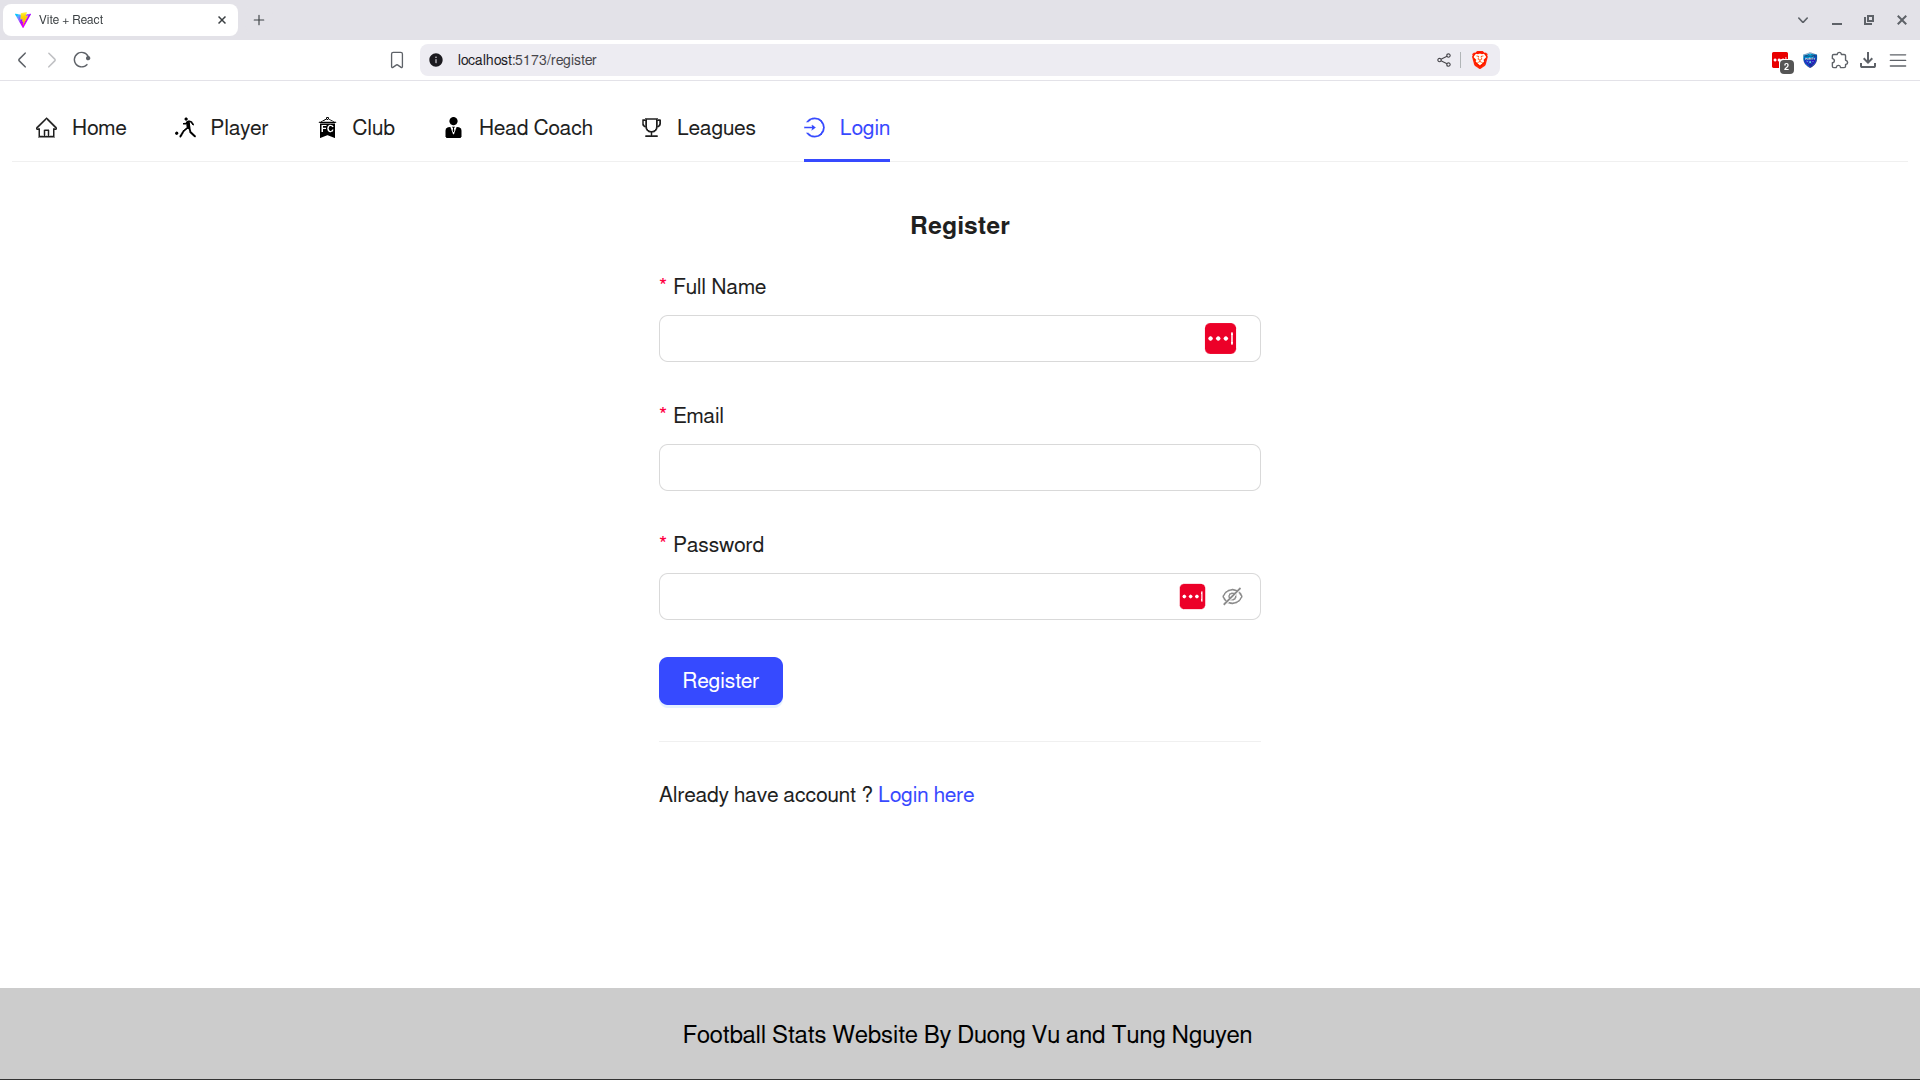
\includegraphics[width=1\linewidth]{Hinhve/user-register.png}
\caption{Giao diện đăng ký người dùng}
\label{fig:user-register}
\end{figure}

\subsubsection{Giao diện đăng nhập}
Giao diện đăng nhập như trên hình \ref{fig:user-login}. Người dùng sử dụng email đã đăng ký và mật khẩu để đăng nhập
\begin{figure}
\centering
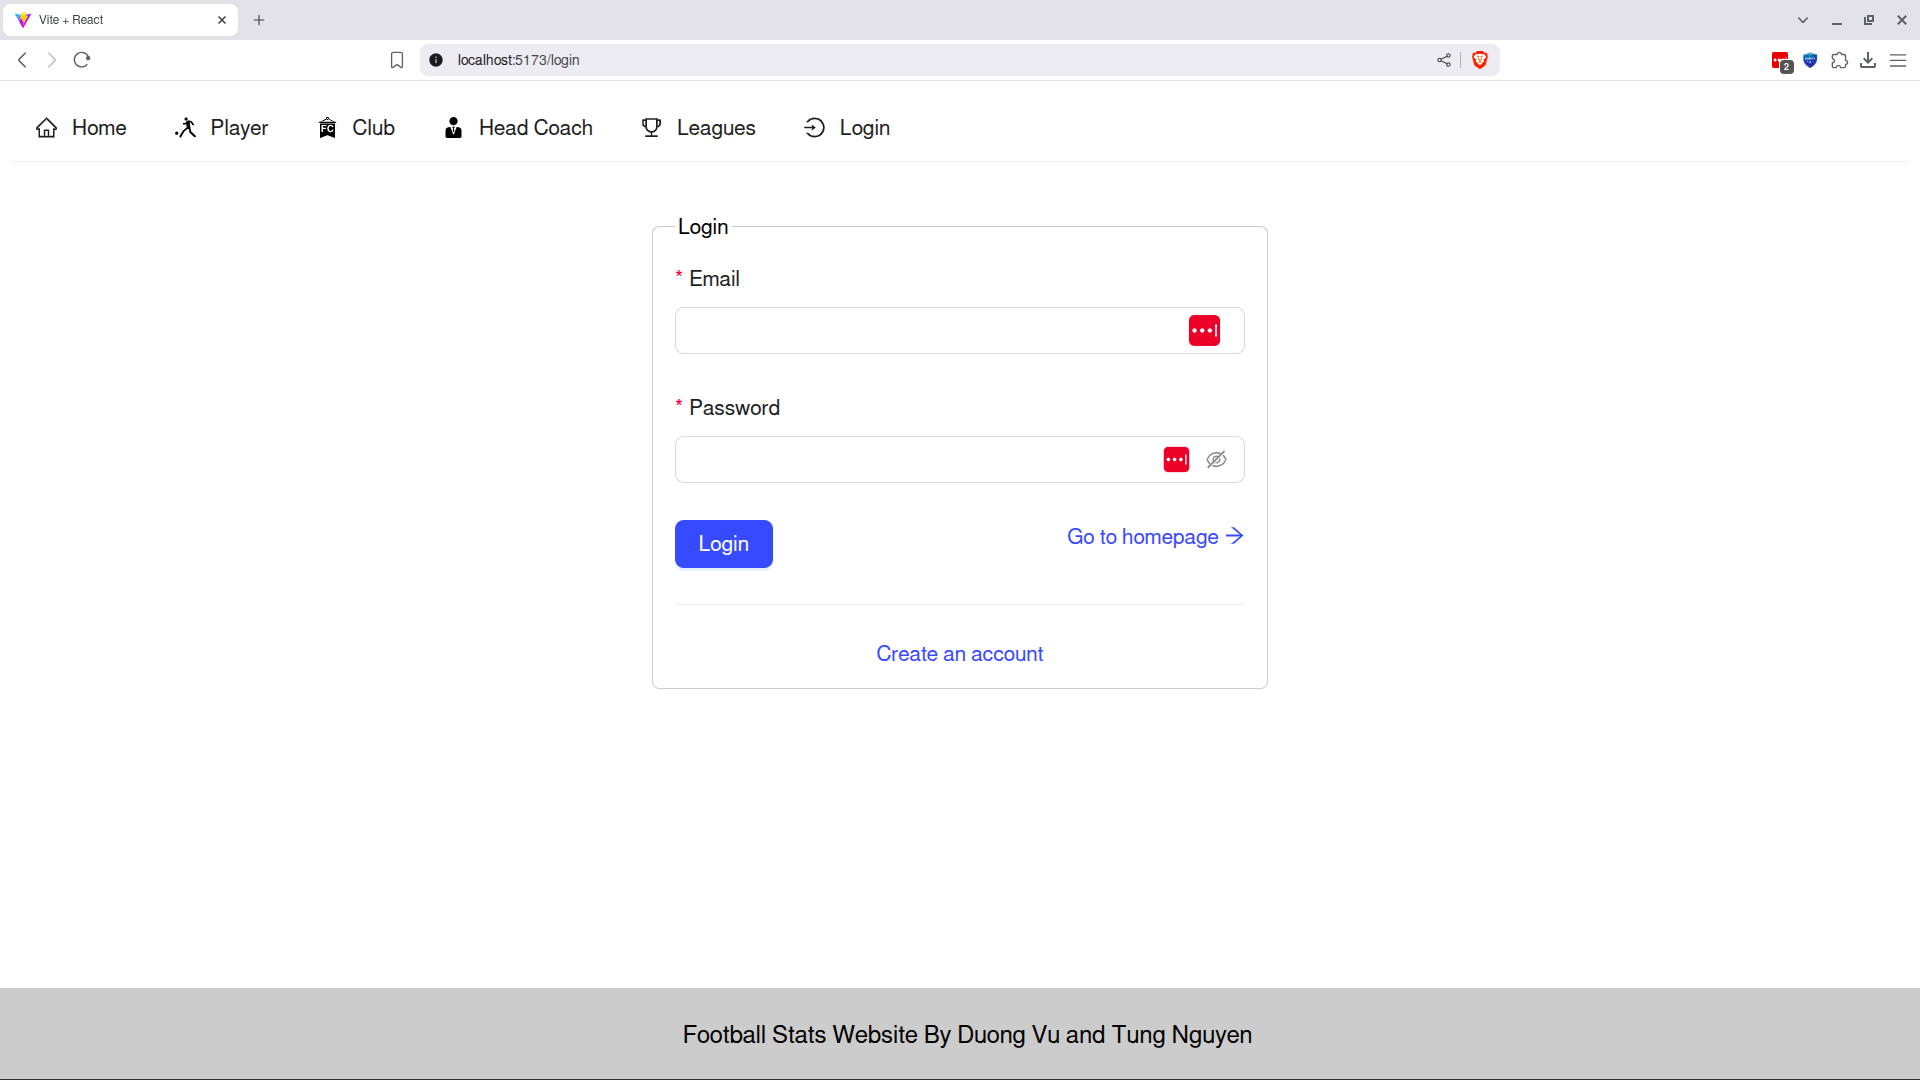
\includegraphics[width=1\linewidth]{Hinhve/user-login.png}
\caption{Giao diện đăng nhập}
\label{fig:user-login}
\end{figure}

\subsubsection{Giao diện trang chủ}
Giao diện trang chủ dành cho người dùng như trên hình \ref{fig:user-home}. Giao diện gồm một thanh tìm kiếm lớn, người dùng chỉ cần nhập một tên bất kỳ của cầu thủ hay câu lạc bộ, huấn luyện viên, giải đấu thì hệ thống đều trả ra kết quả của cả 4 thực thể.
\begin{figure}
    \centering
    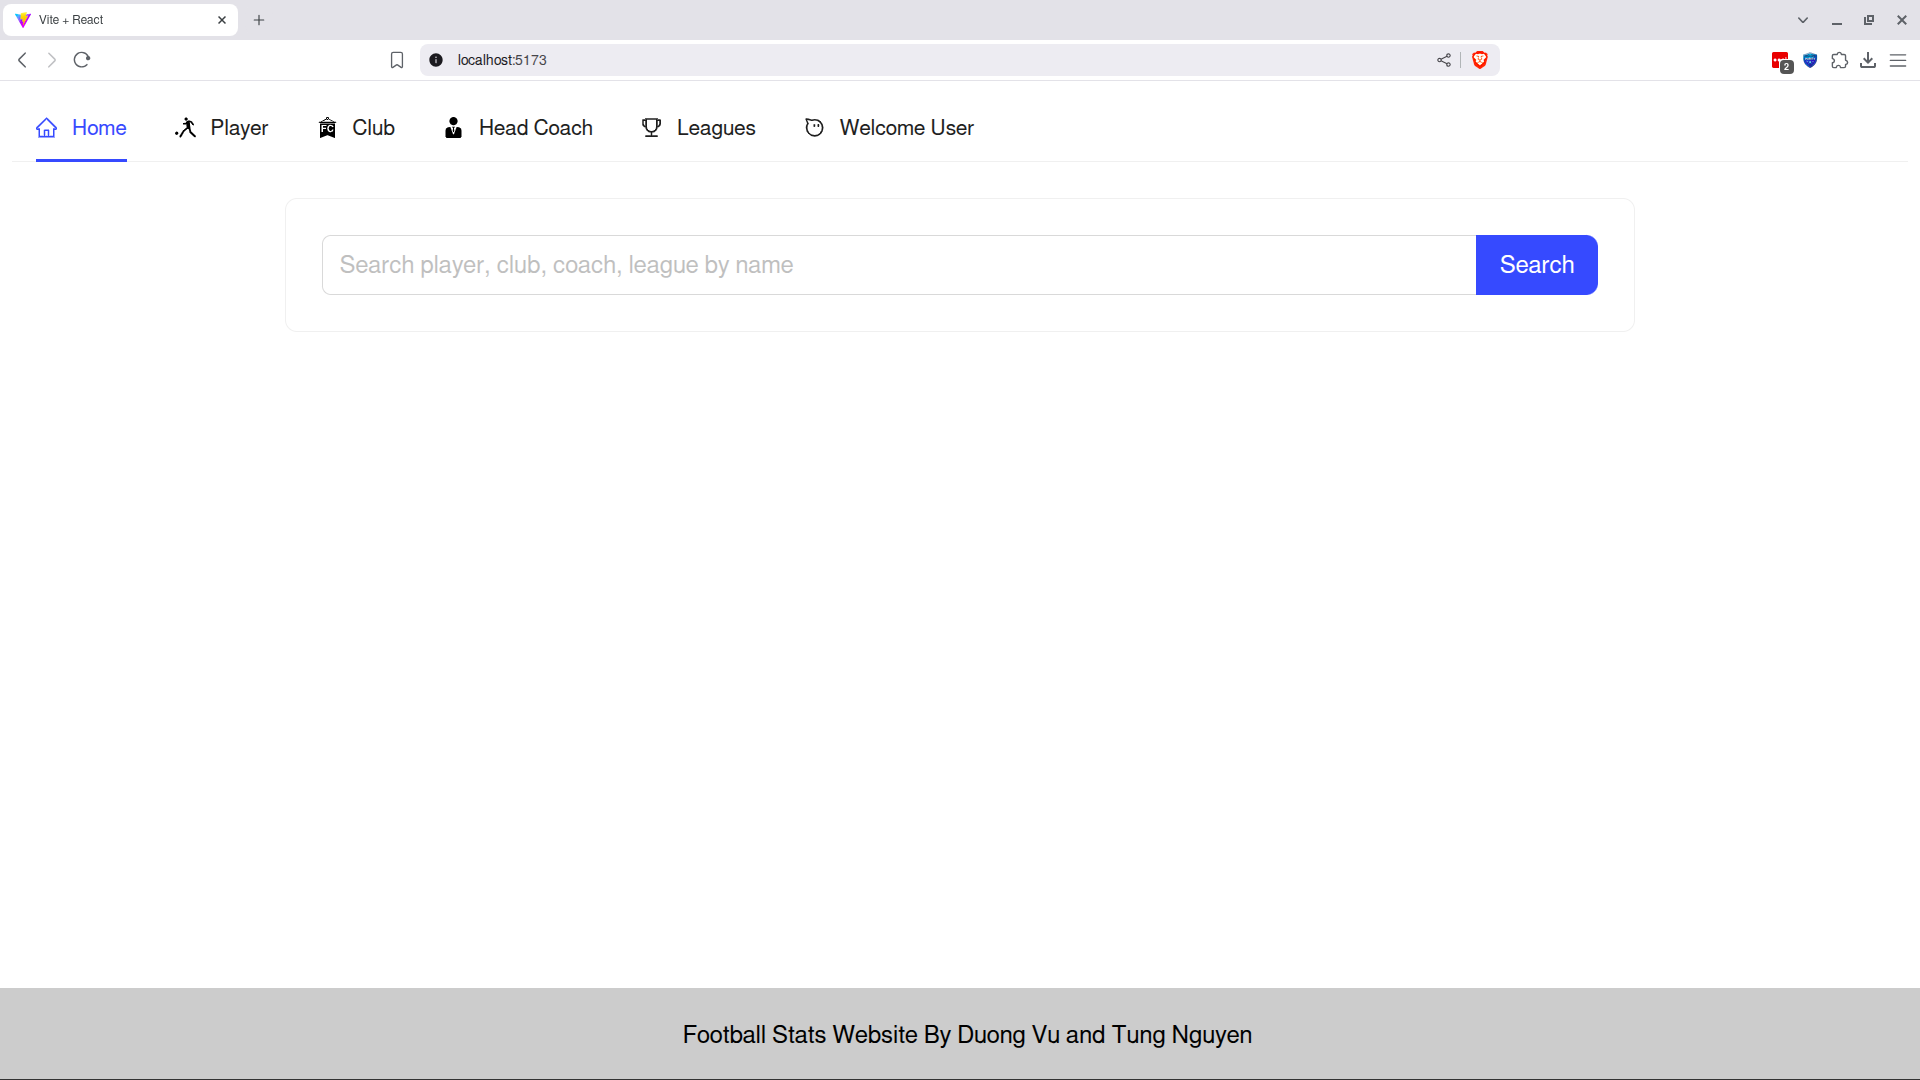
\includegraphics[width=1\linewidth]{Hinhve/user-home.png}
    \caption{Giao diện trang chủ dành cho người dùng}
    \label{fig:user-home}
\end{figure}
\subsection{ Giao diện cầu thủ}
\subsubsection{Giao diện danh sách cầu thủ}
Giao diện danh sách cầu thủ như trên hình \ref{fig:user-player-list}. Giao diện có chức năng phân trang và chức năng lọc theo các tiêu chí
\begin{figure}
\centering
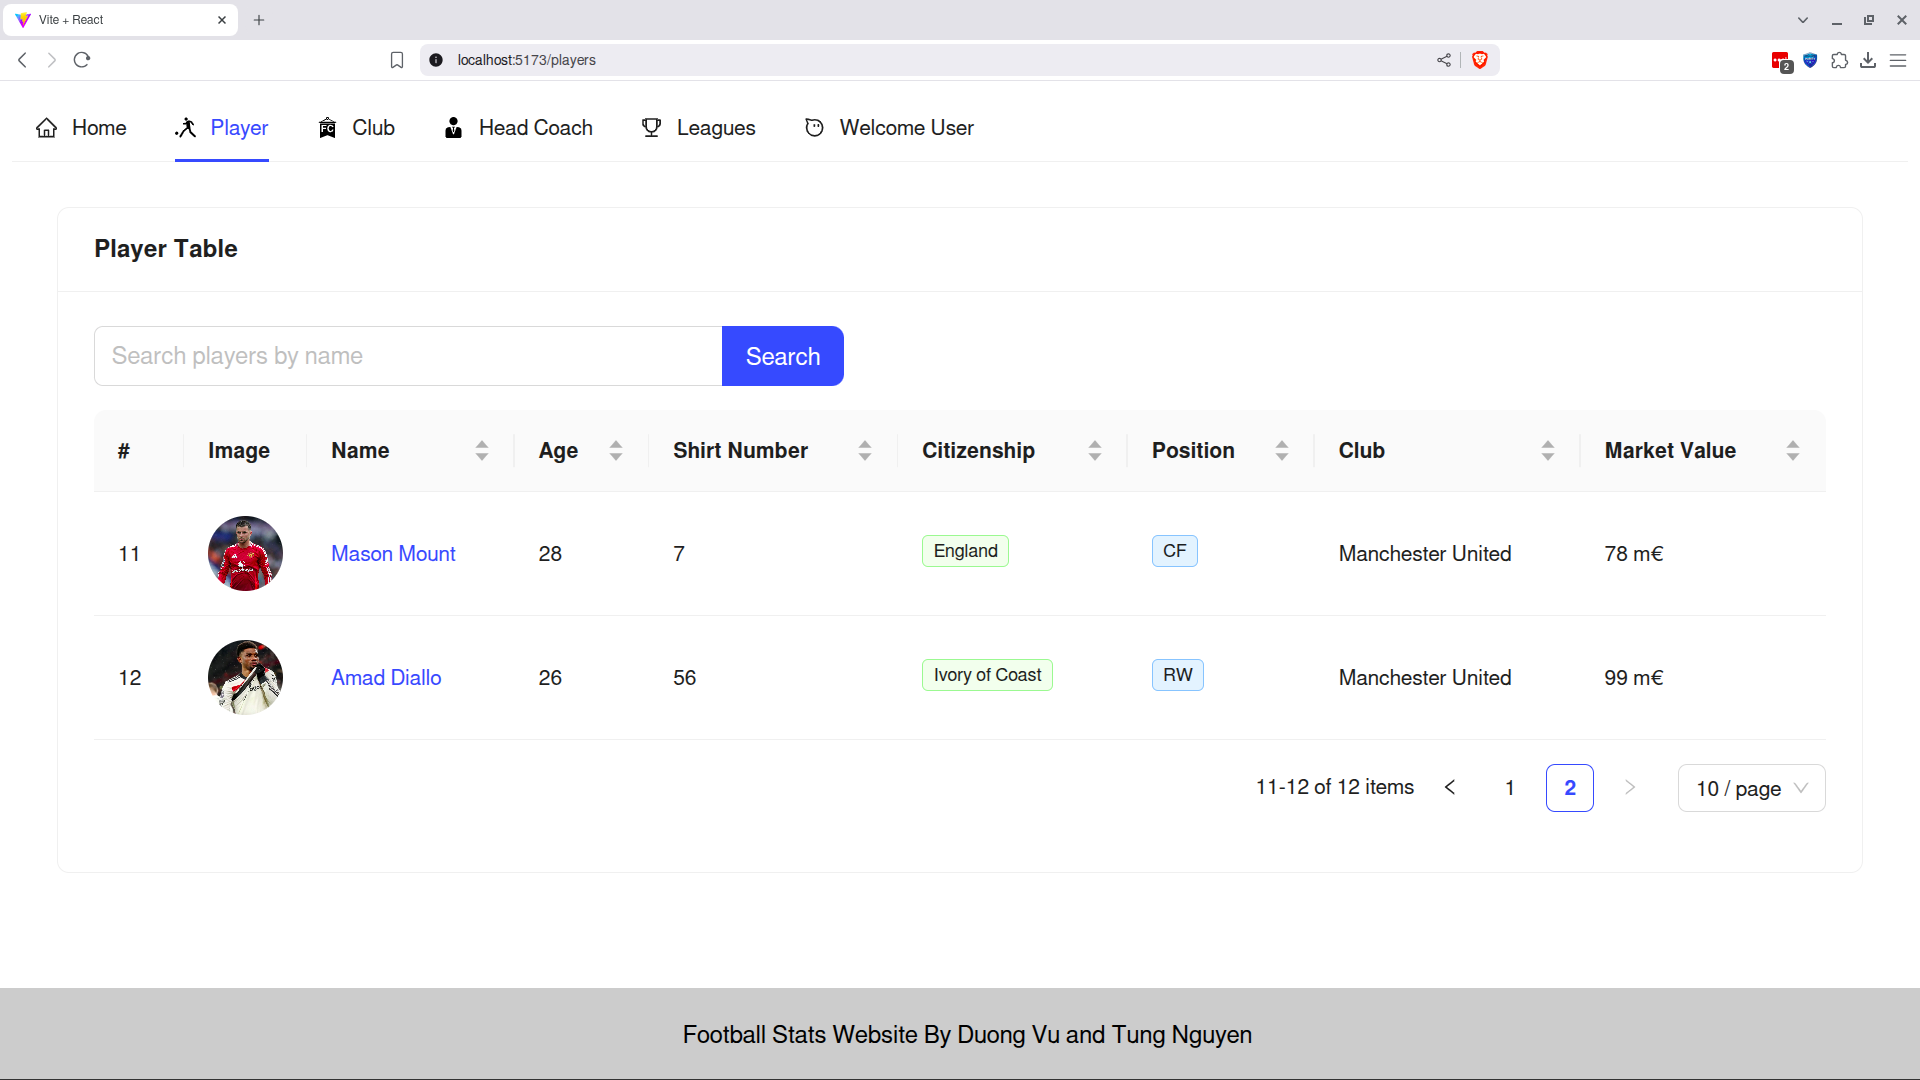
\includegraphics[width=1\linewidth]{Hinhve/user-player-list.png}
\caption{Giao diện danh sách cầu thủ}
\label{fig:user-player-list}
\end{figure}

\subsubsection{Giao diện lọc cầu thủ}
Giao diện lọc cầu thủ như trên hình \ref{fig:user-player-filter}.
\begin{figure}
\centering
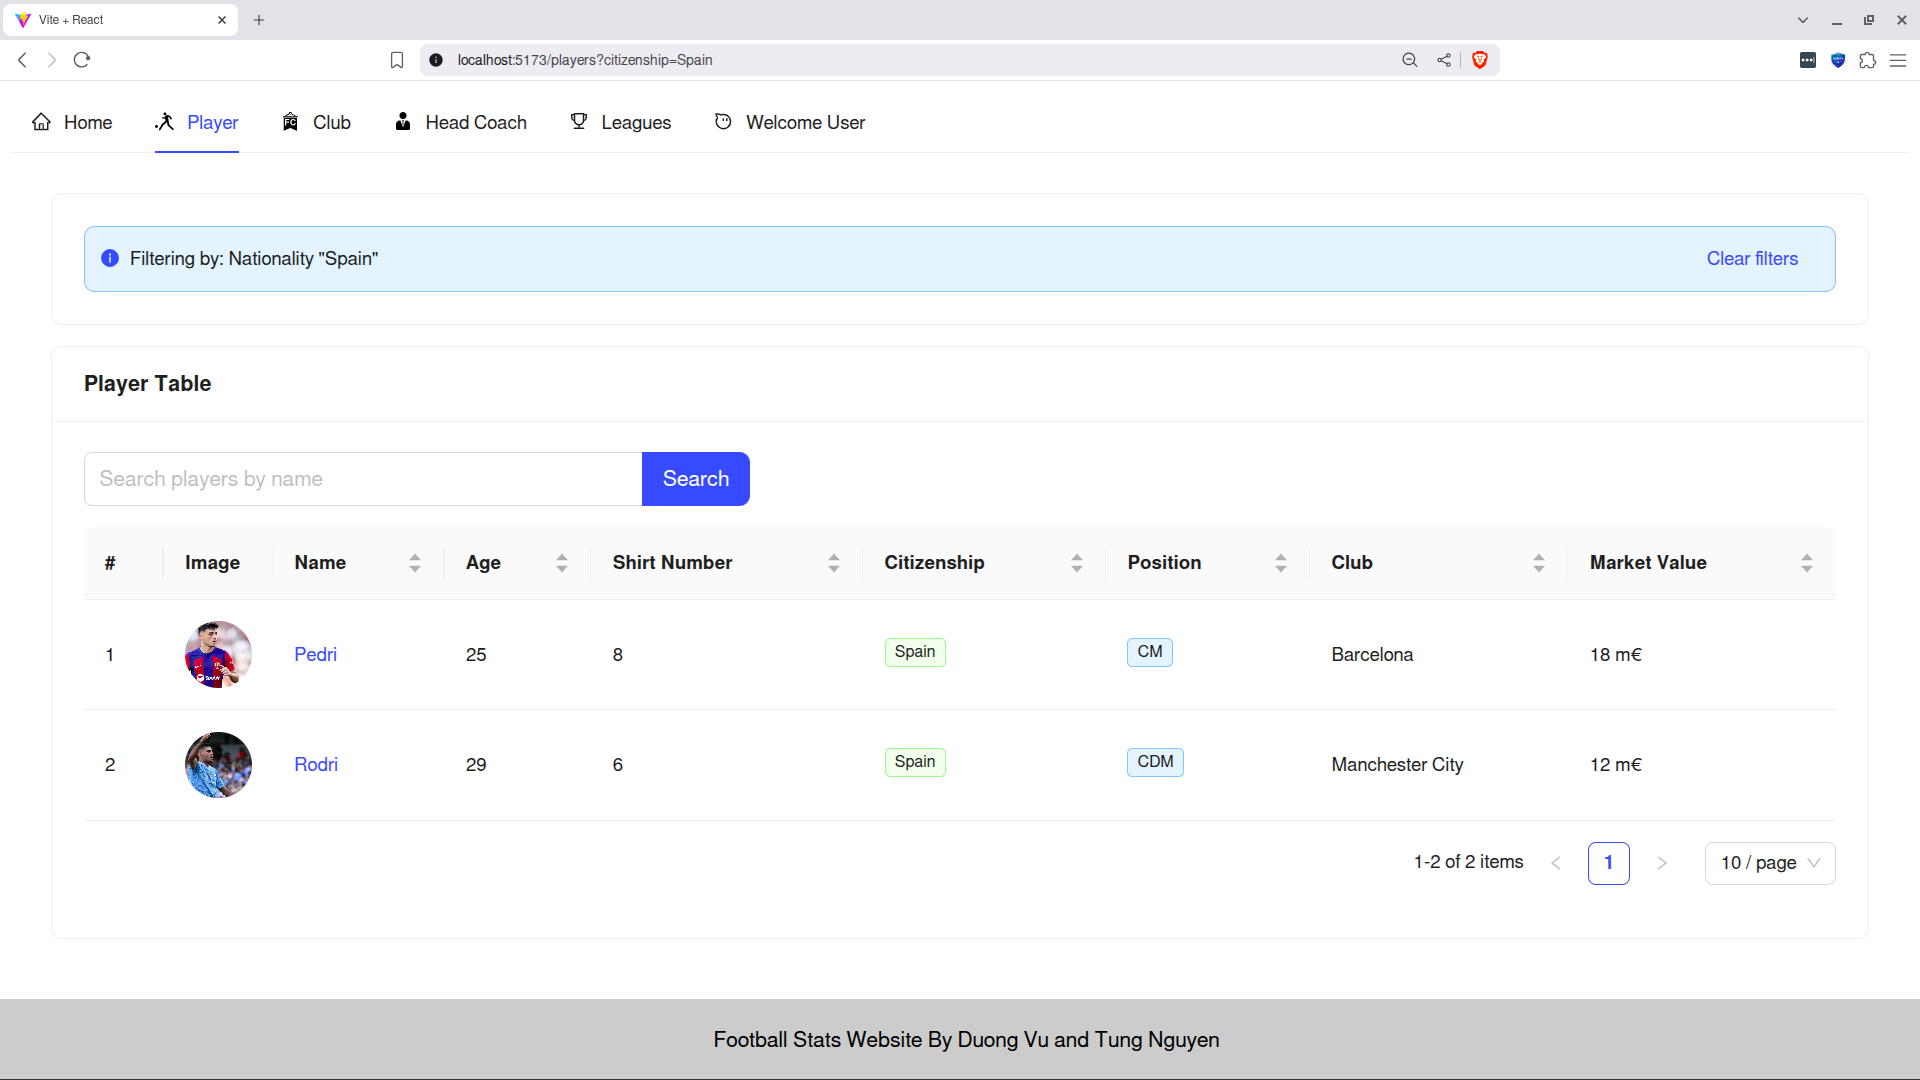
\includegraphics[width=1\linewidth]{Hinhve/user-player-filter.png}
\caption{Giao diện lọc cầu thủ}
\label{fig:user-player-filter}
\end{figure}

\subsubsection{Giao diện chi tiết cầu thủ}
Giao diện chi tiết cầu thủ như trên hình \ref{fig:user-player-detail}.
\begin{figure}
\centering
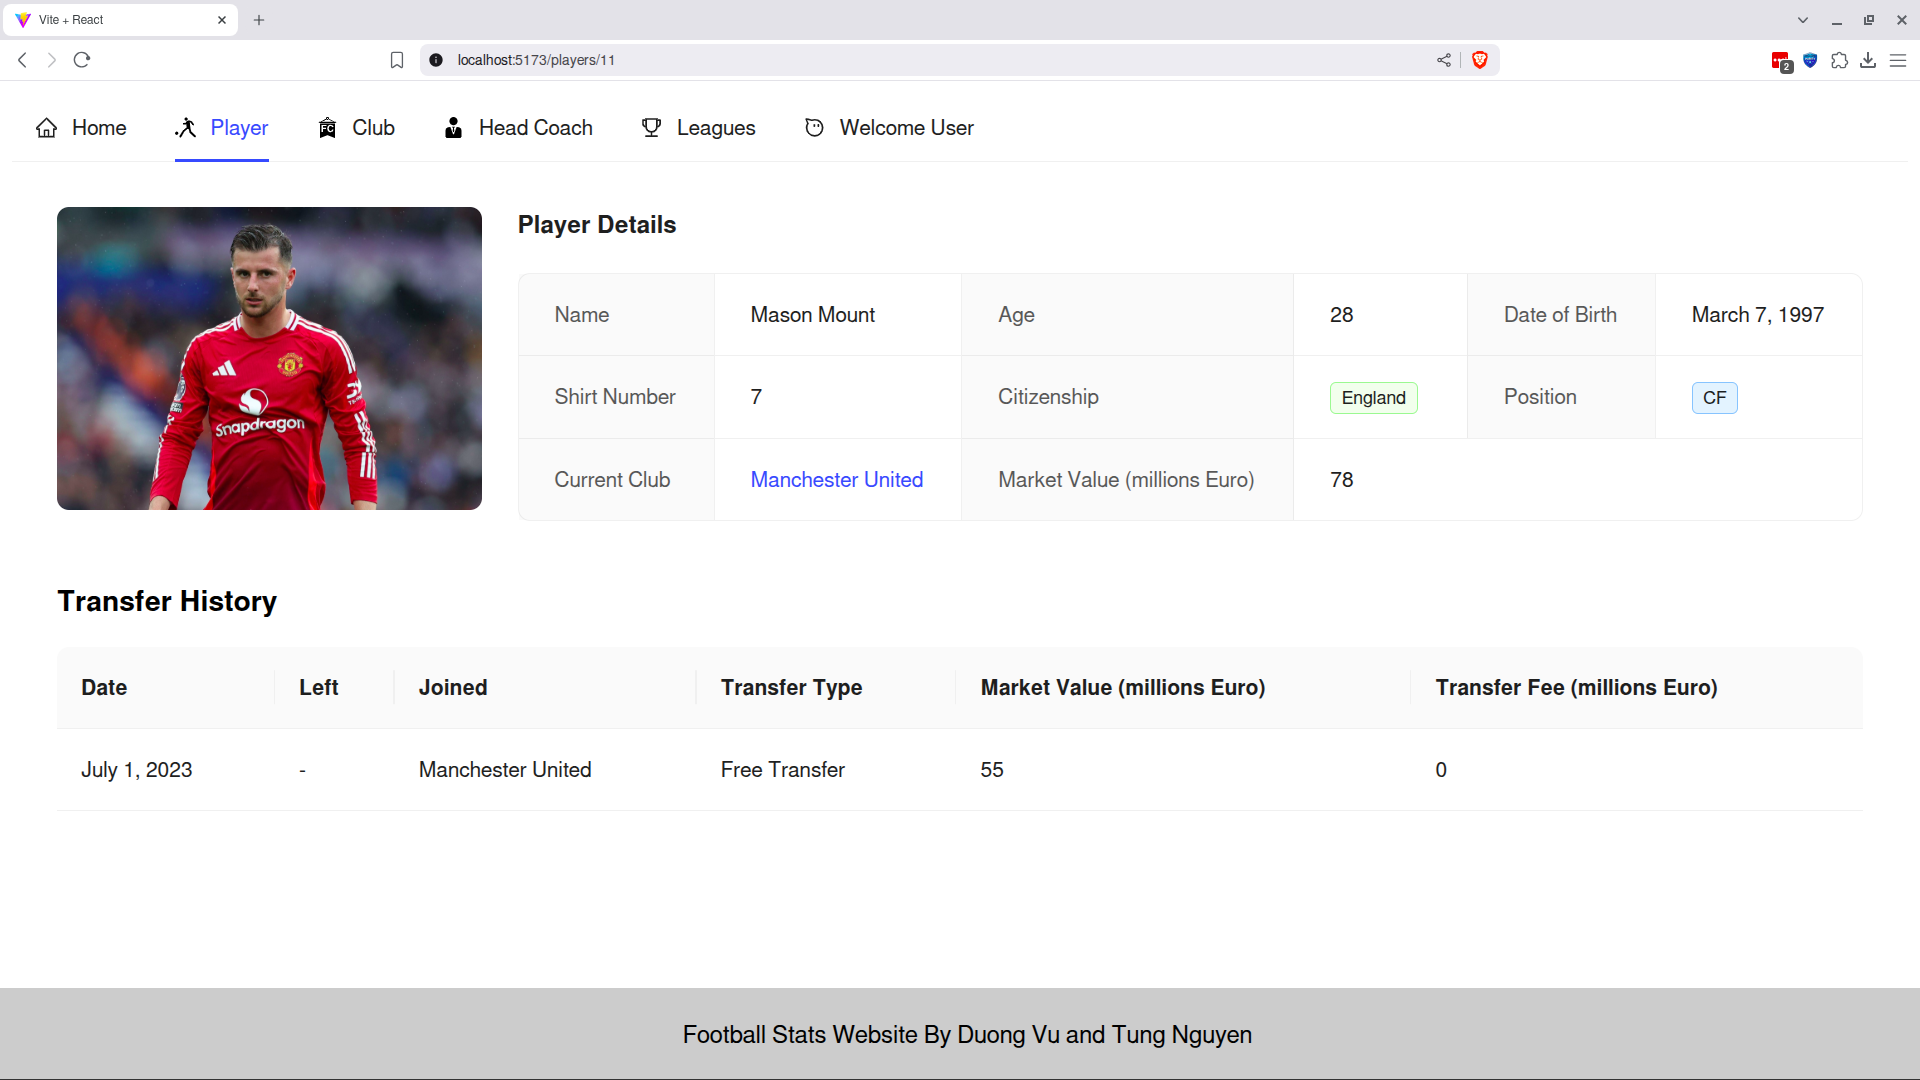
\includegraphics[width=1\linewidth]{Hinhve/user-player-detail.png}
\caption{Giao diện chi tiết cầu thủ}
\label{fig:user-player-detail}
\end{figure}

\subsubsection{Giao diện tìm kiếm cầu thủ}
Giao diện tìm kiếm cầu thủ như trên hình \ref{fig:user-player-search}.
\begin{figure}
\centering
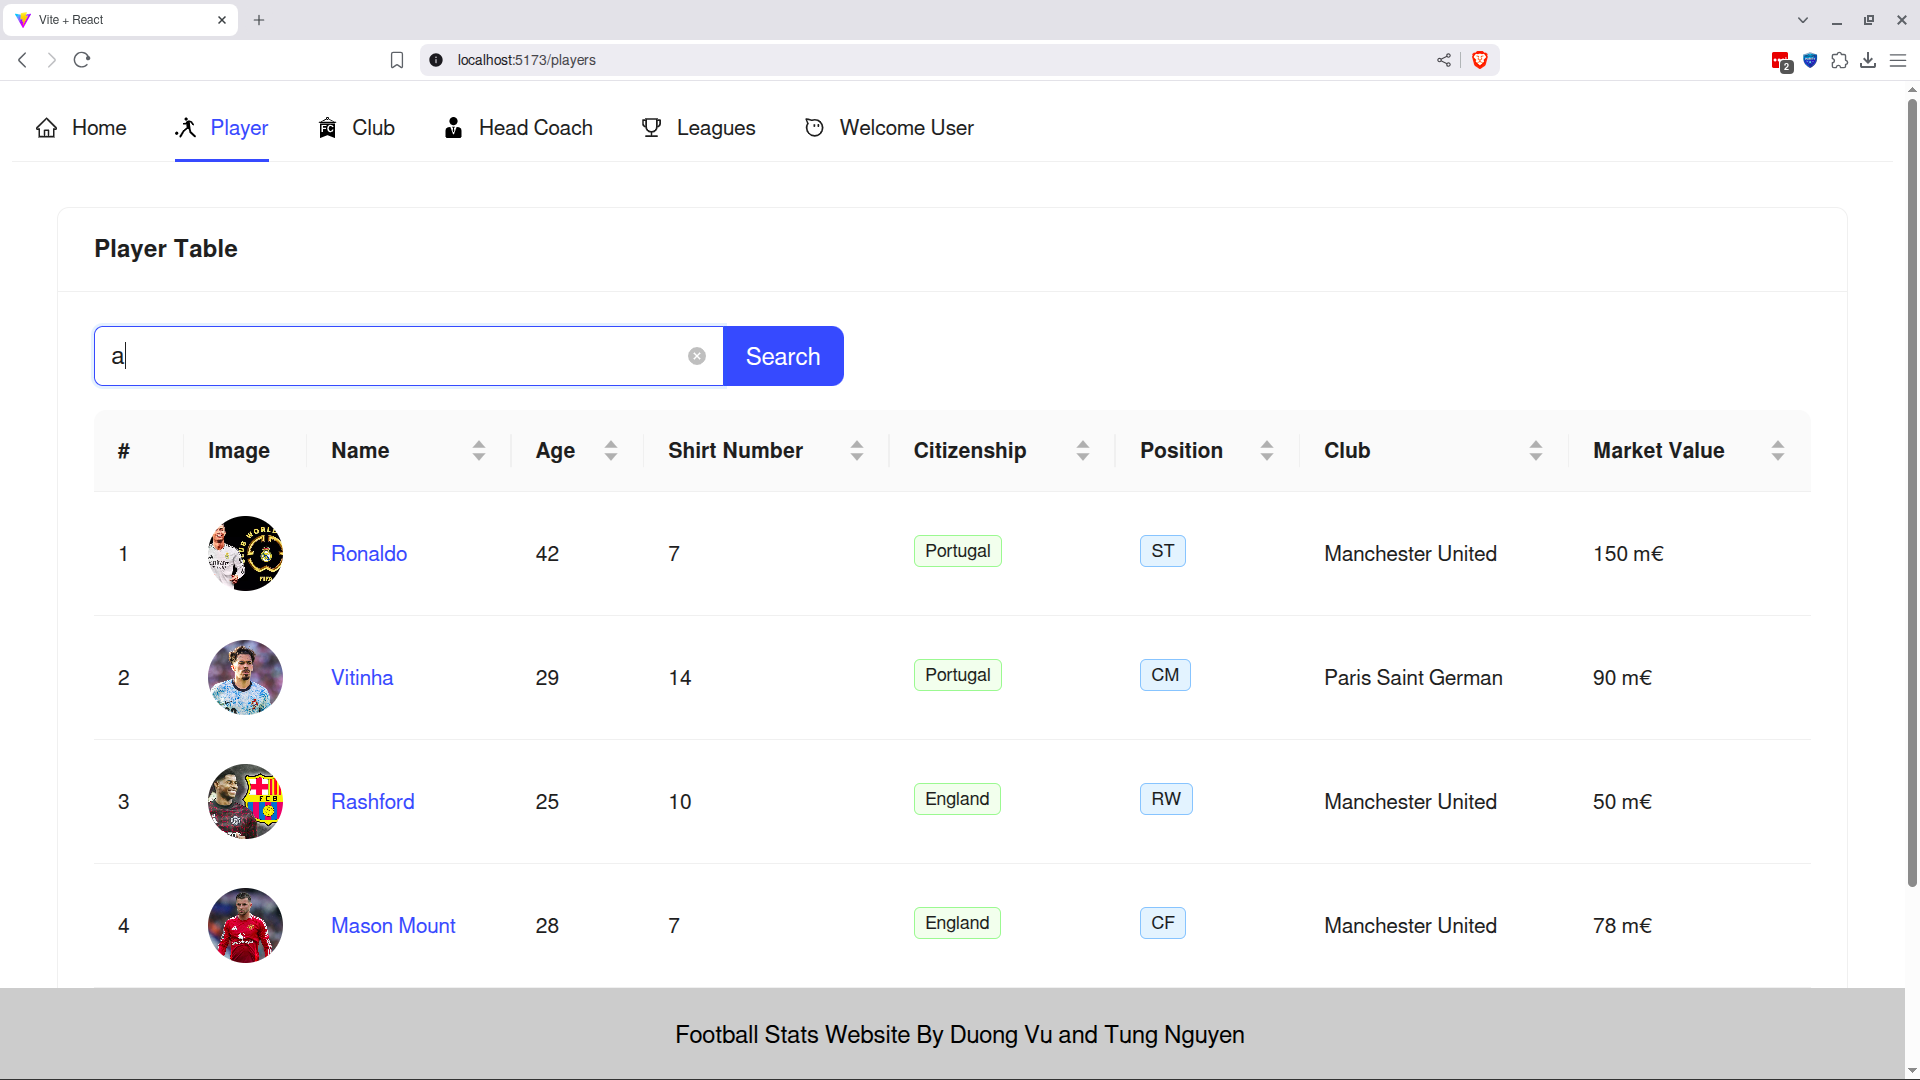
\includegraphics[width=1\linewidth]{Hinhve/user-player-search.png}
\caption{Giao diện tìm kiếm cầu thủ}
\label{fig:user-player-search}
\end{figure}
\subsection{ Giao diện câu lạc bộ}
\subsubsection{Giao diện danh sách câu lạc bộ}
Giao diện danh sách câu lạc bộ như trên hình \ref{fig:user-club-list}.
\begin{figure}
\centering
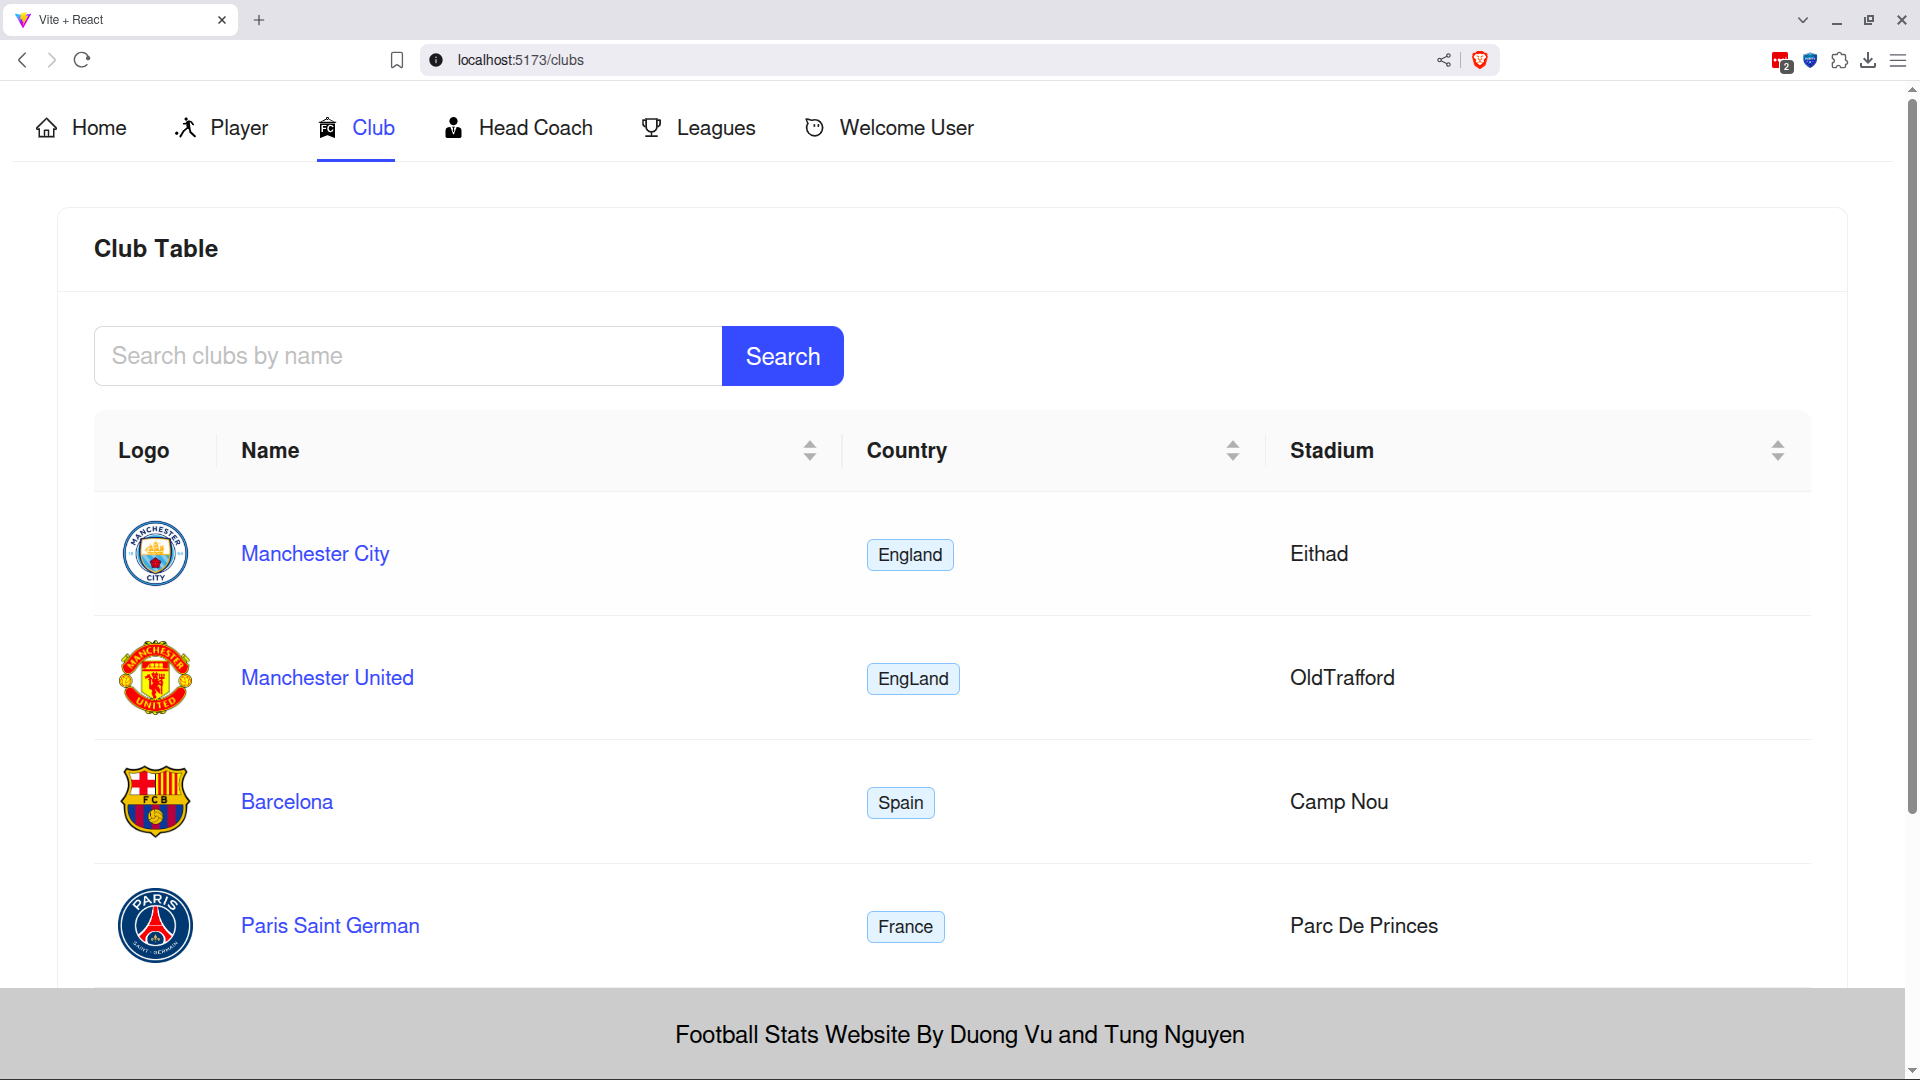
\includegraphics[width=1\linewidth]{Hinhve/user-club-list.png}
\caption{Giao diện danh sách câu lạc bộ}
\label{fig:user-club-list}
\end{figure}
\subsubsection{Giao diện tìm kiếm câu lạc bộ}
Giao diện tìm kiếm câu lạc bộ như trên hình \ref{fig:user-club-search}.
\begin{figure}
\centering
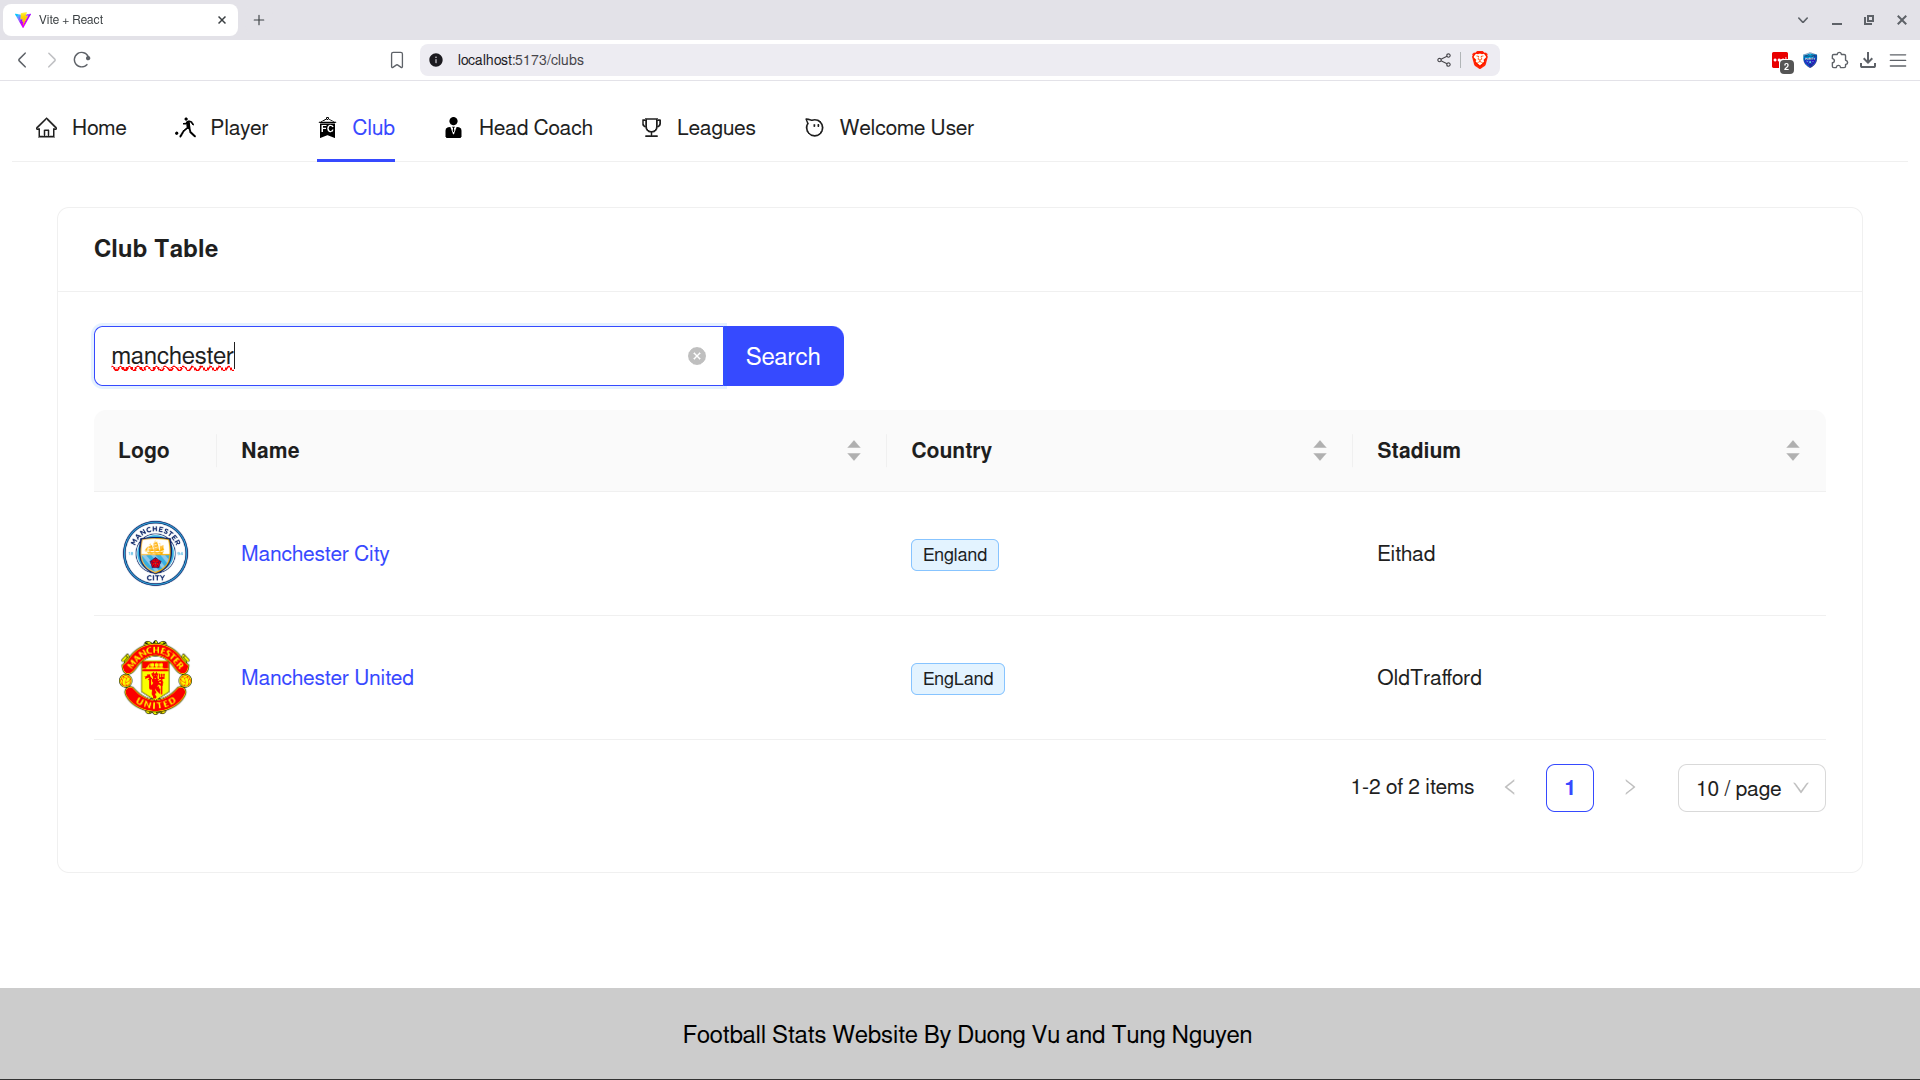
\includegraphics[width=1\linewidth]{Hinhve/user-club-search.png}
\caption{Giao diện tìm kiếm câu lạc bộ}
\label{fig:user-club-search}
\end{figure}

\subsubsection{Giao diện lọc câu lạc bộ}
Giao diện lọc câu lạc bộ như trên hình \ref{fig:user-club-filter}.
\begin{figure}
\centering
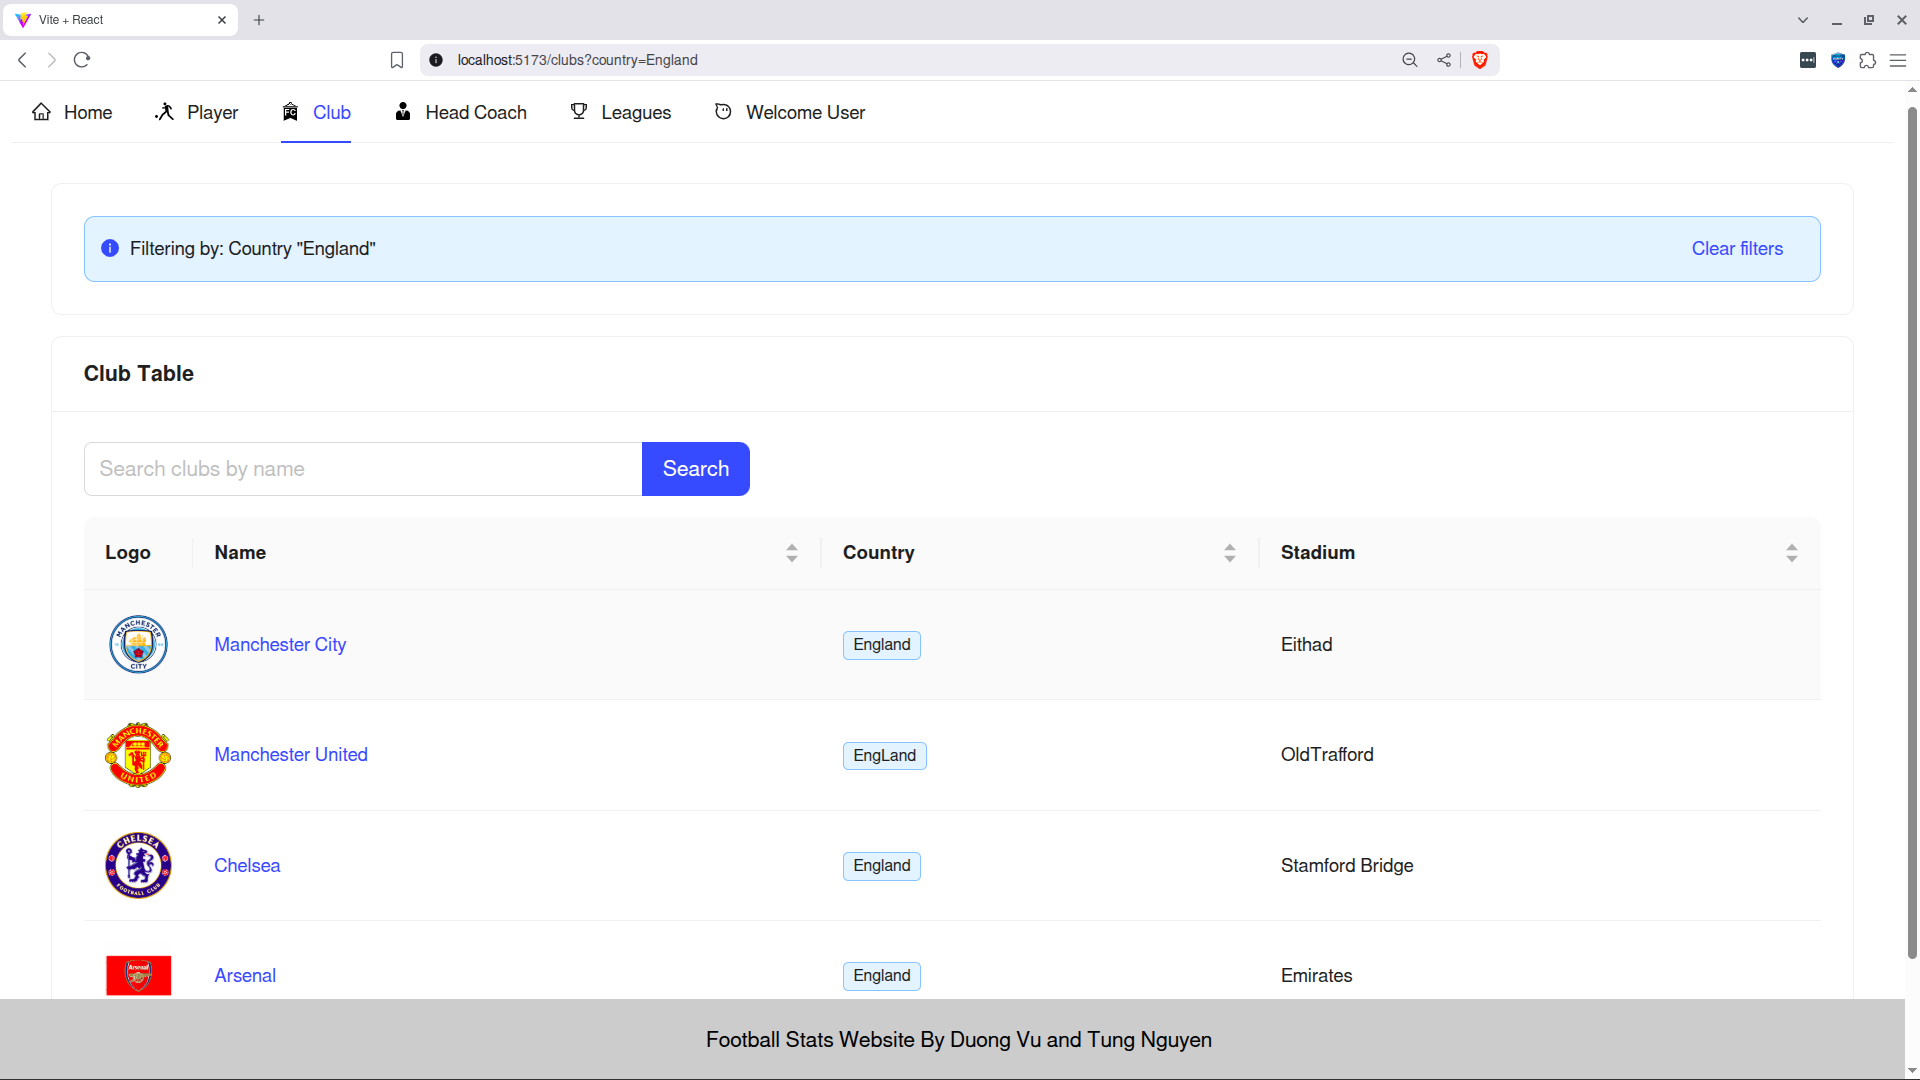
\includegraphics[width=1\linewidth]{Hinhve/user-club-filter.png}
\caption{Giao diện lọc câu lạc bộ}
\label{fig:user-club-filter}
\end{figure}

\subsubsection{Giao diện chi tiết danh sách cầu thủ trong mùa giải của câu lạc bộ}
Giao diện chi tiết danh sách cầu thủ trong mùa giải của câu lạc bộ như trên hình \ref{fig:user-club-detail-squad}.
\begin{figure}
\centering
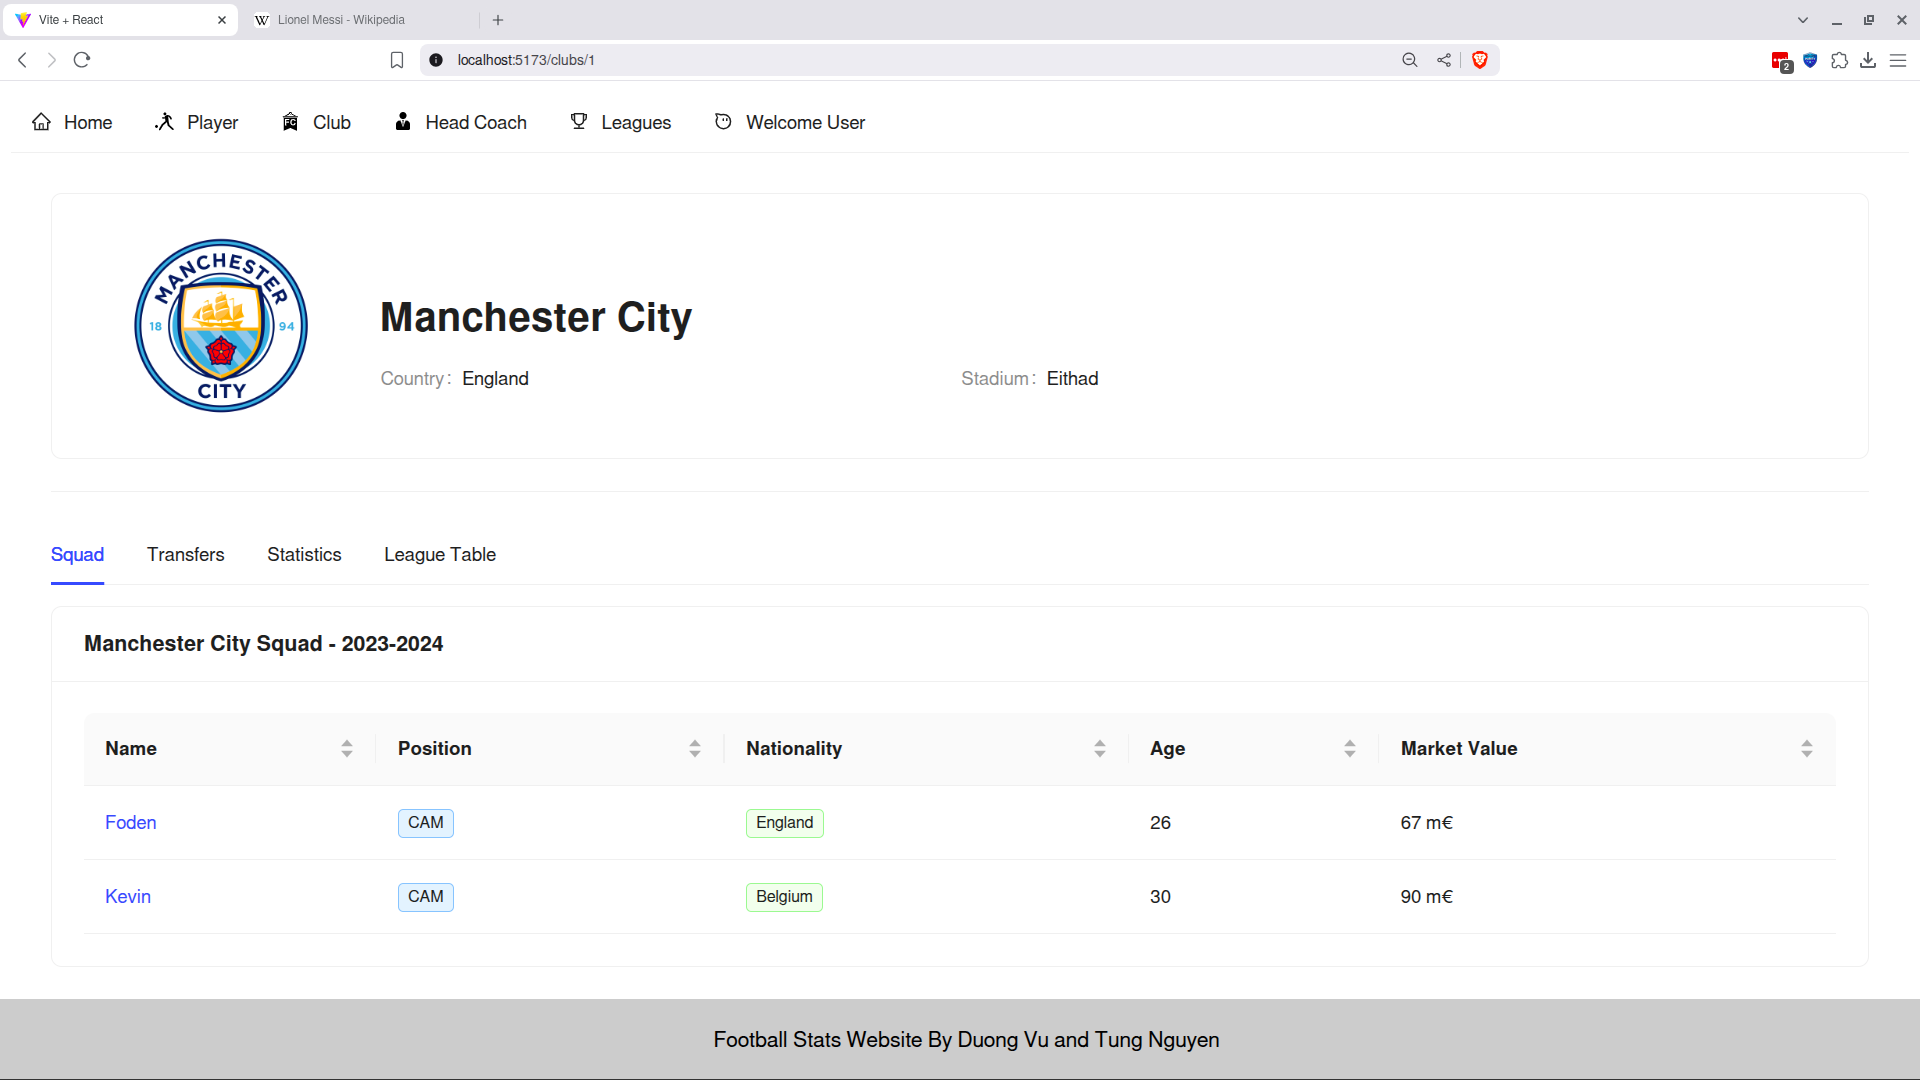
\includegraphics[width=1\linewidth]{Hinhve/user-club-detail-squad.png}
\caption{Giao diện chi tiết danh sách cầu thủ trong mùa giải của câu lạc bộ}
\label{fig:user-club-detail-squad}
\end{figure}

\subsubsection{Giao diện chi tiết danh sách chuyển nhượng trong mùa giải của câu lạc bộ}
Giao diện chi tiết chuyển nhượng trong mùa giải của câu lạc bộ như trên hình \ref{fig:user-club-detail-transfer}.
\begin{figure}
\centering
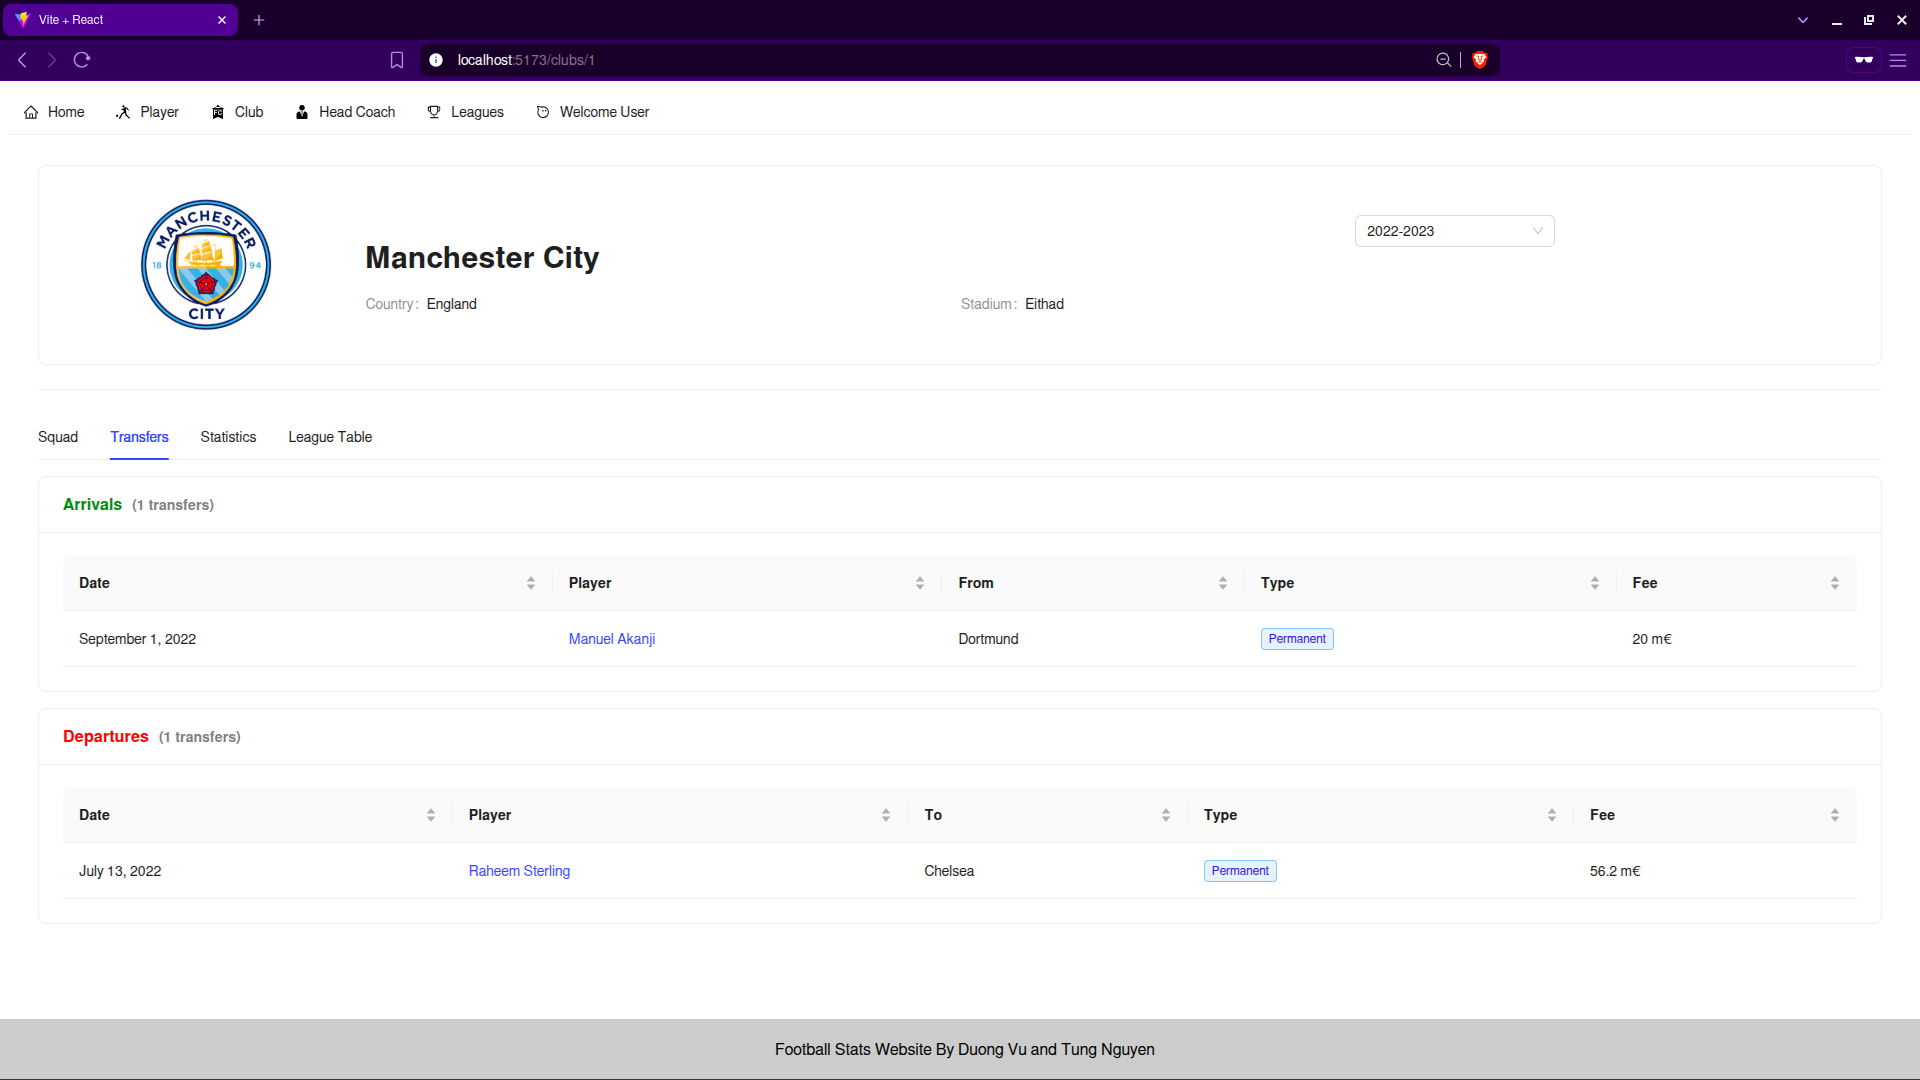
\includegraphics[width=1\linewidth]{Hinhve/user-club-detail-transfer.png}
\caption{Giao diện chi tiết chuyển nhượng trong mùa giải của câu lạc bộ}
\label{fig:user-club-detail-transfer}
\end{figure}

\subsubsection{Giao diện chi tiết thống kê trong mùa giải của câu lạc bộ}
Giao diện chi tiết thống kê trong mùa giải của câu lạc bộ như trên hình \ref{fig:user-club-detail-statistic}.
\begin{figure}
\centering
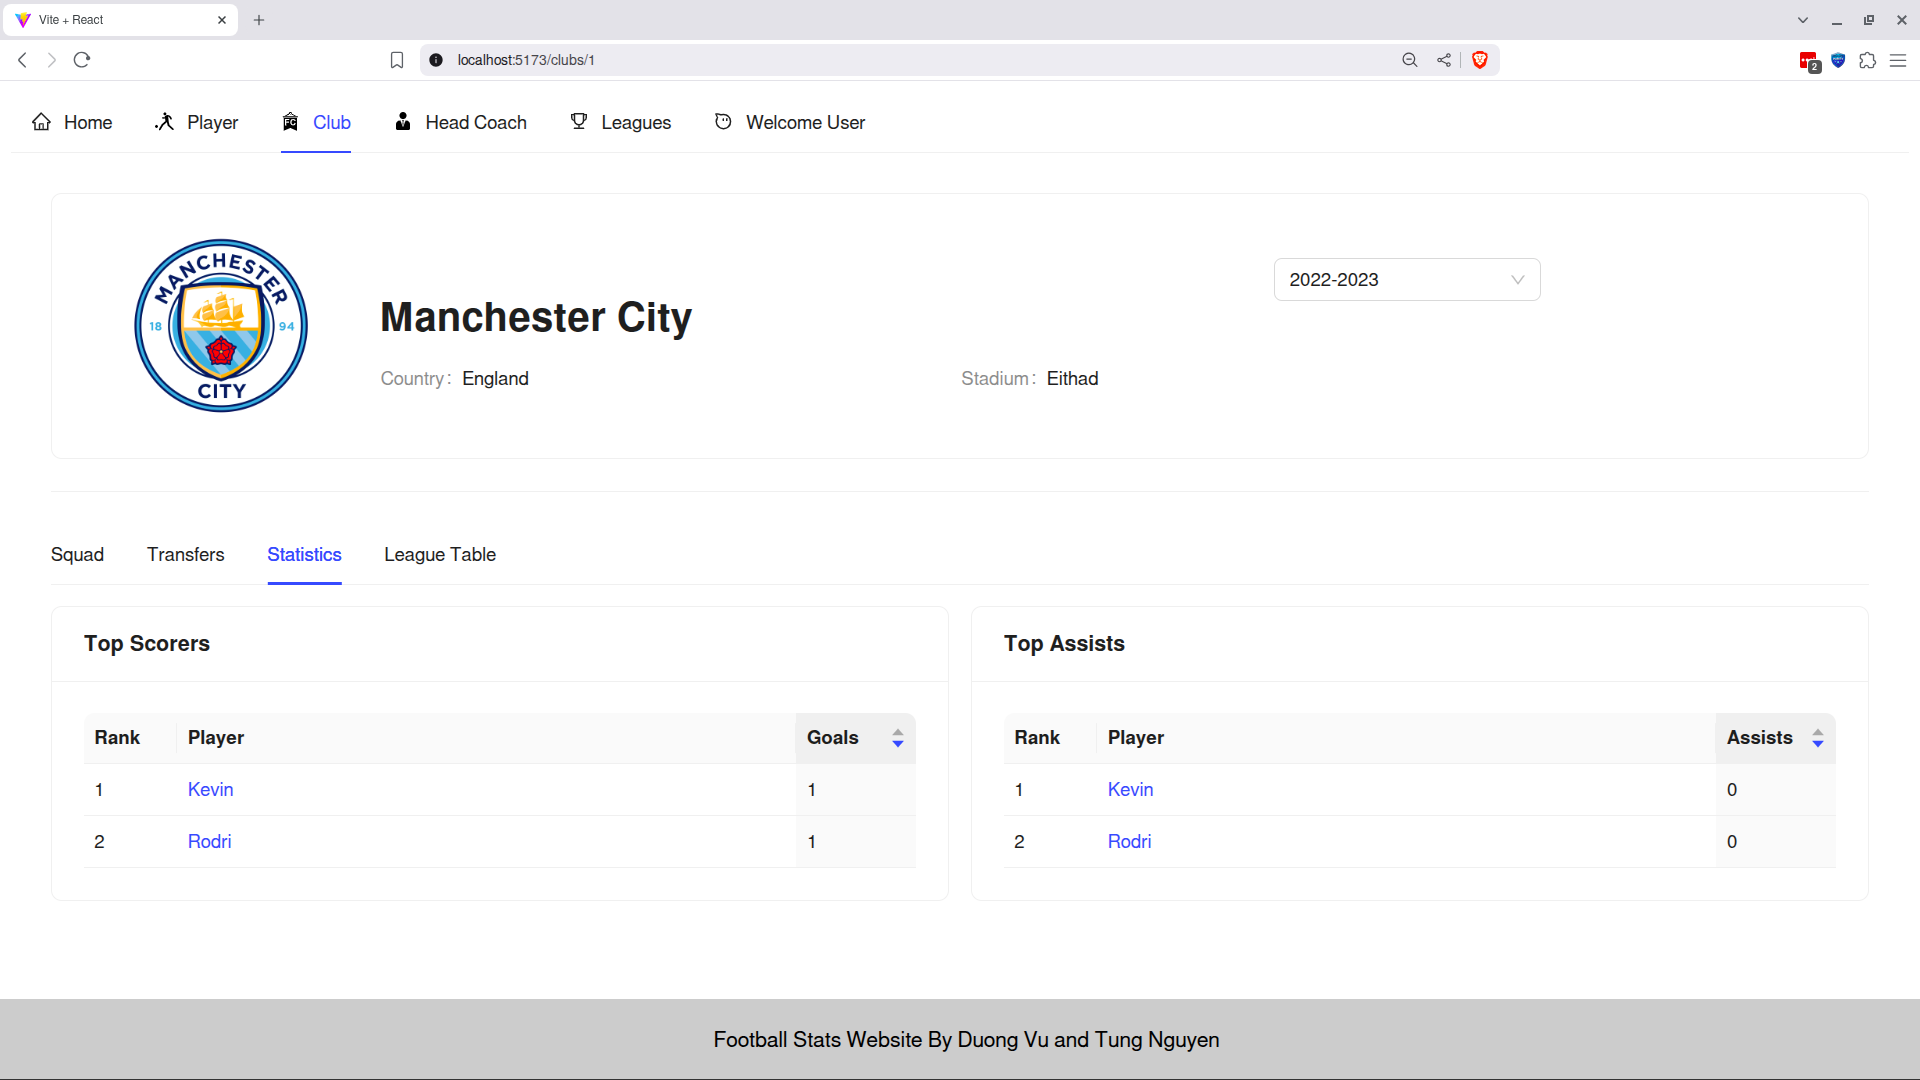
\includegraphics[width=1\linewidth]{Hinhve/user-club-detail-statistic.png}
\caption{Giao diện chi tiết thống kê trong mùa giải của câu lạc bộ}
\label{fig:user-club-detail-statistic}
\end{figure}

\subsubsection{Giao diện chi tiết thứ hạng câu lạc bộ trong mùa giải}
Giao diện chi tiết thứ hạng câu lạc bộ trong mùa giải như trên hình \ref{fig:user-club-detail-league-table}.
\begin{figure}
\centering
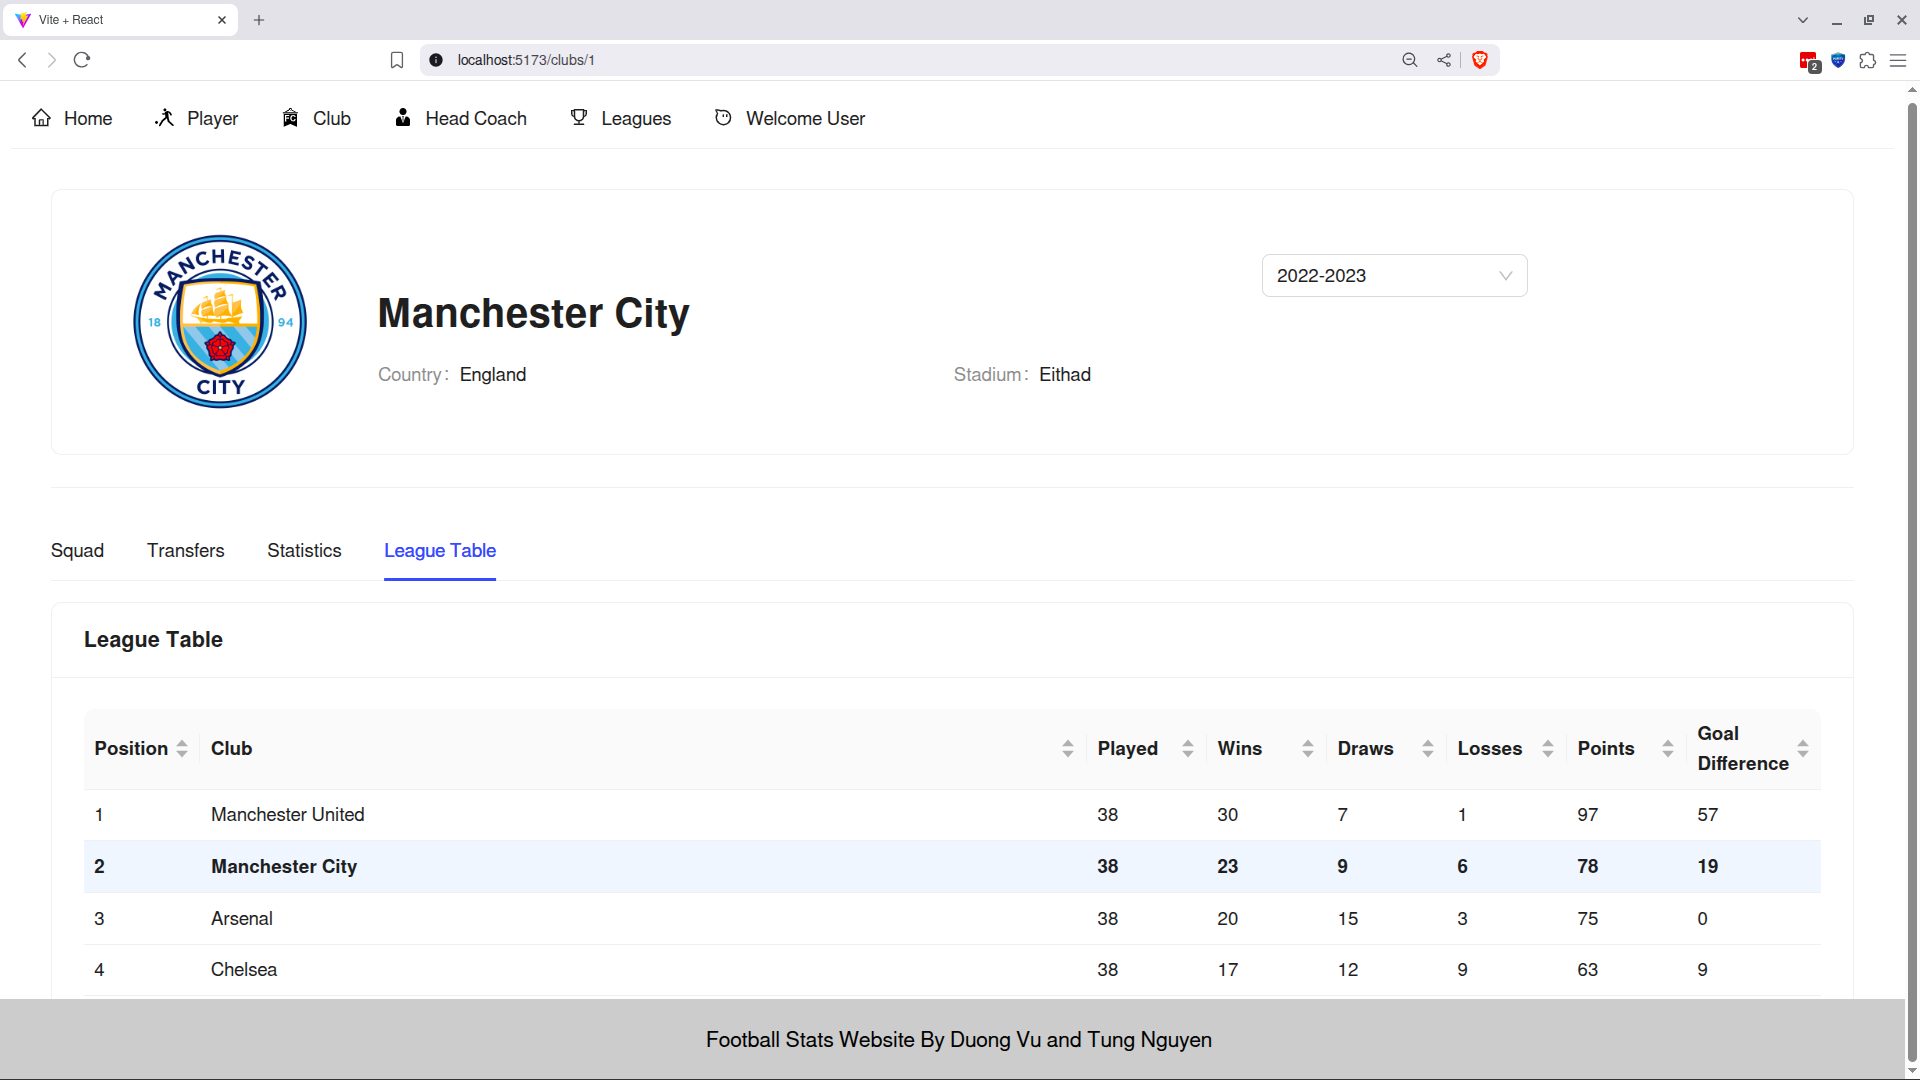
\includegraphics[width=1\linewidth]{Hinhve/user-club-detail-league-table.png}
\caption{Giao diện chi tiết thứ hạng câu lạc bộ trong mùa giải}
\label{fig:user-club-detail-league-table}
\end{figure}

\subsection{ Giao diện huấn luyện viên}
\subsubsection{Giao diện danh sách huấn luyện viên}
Giao diện danh sách huấn luyện viên như trên hình \ref{fig:user-coach-list}.
\begin{figure}
\centering
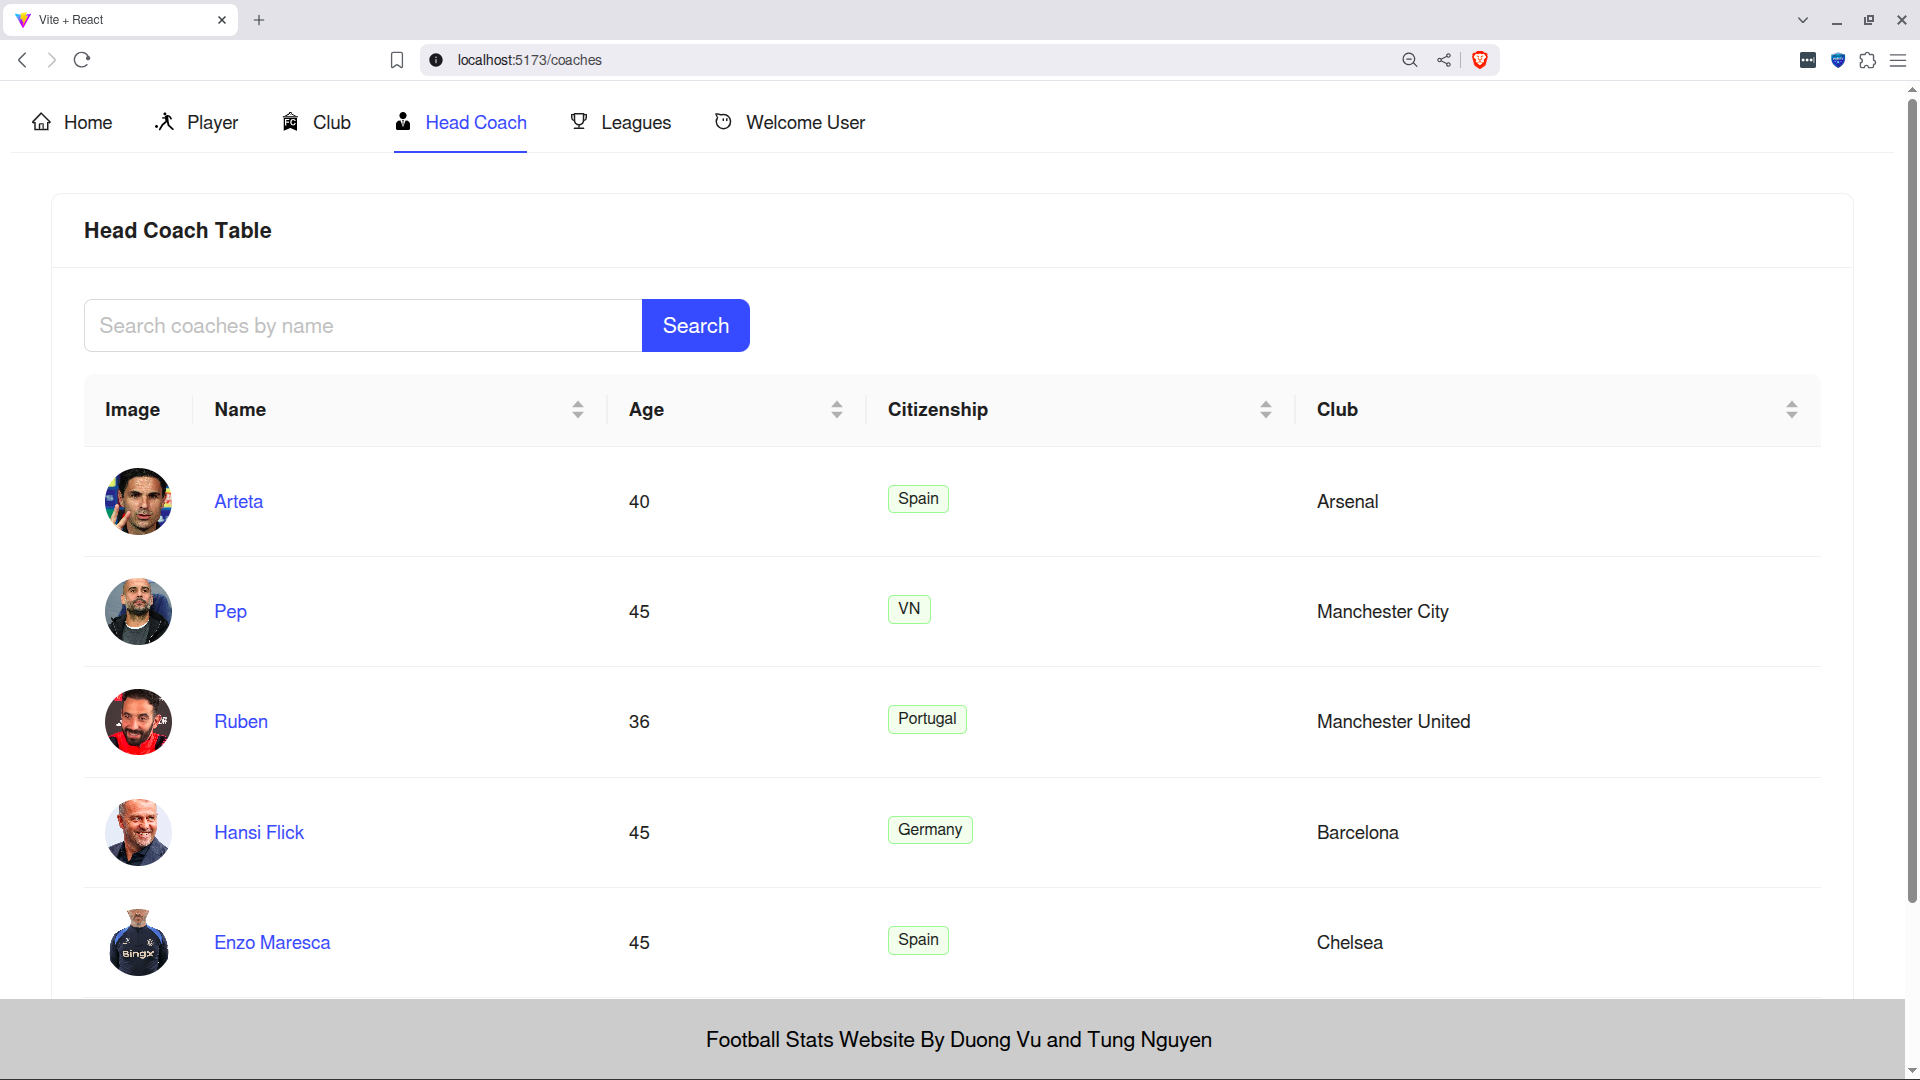
\includegraphics[width=1\linewidth]{Hinhve/user-coach-list.png}
\caption{Giao diện danh sách huấn luyện viên}
\label{fig:user-coach-list}
\end{figure}


\subsubsection{Giao diện tìm kiếm huấn luyện viên}
Giao diện tìm kiếm huấn luyện viên như trên hình \ref{fig:user-coach-search}.
\begin{figure}
\centering
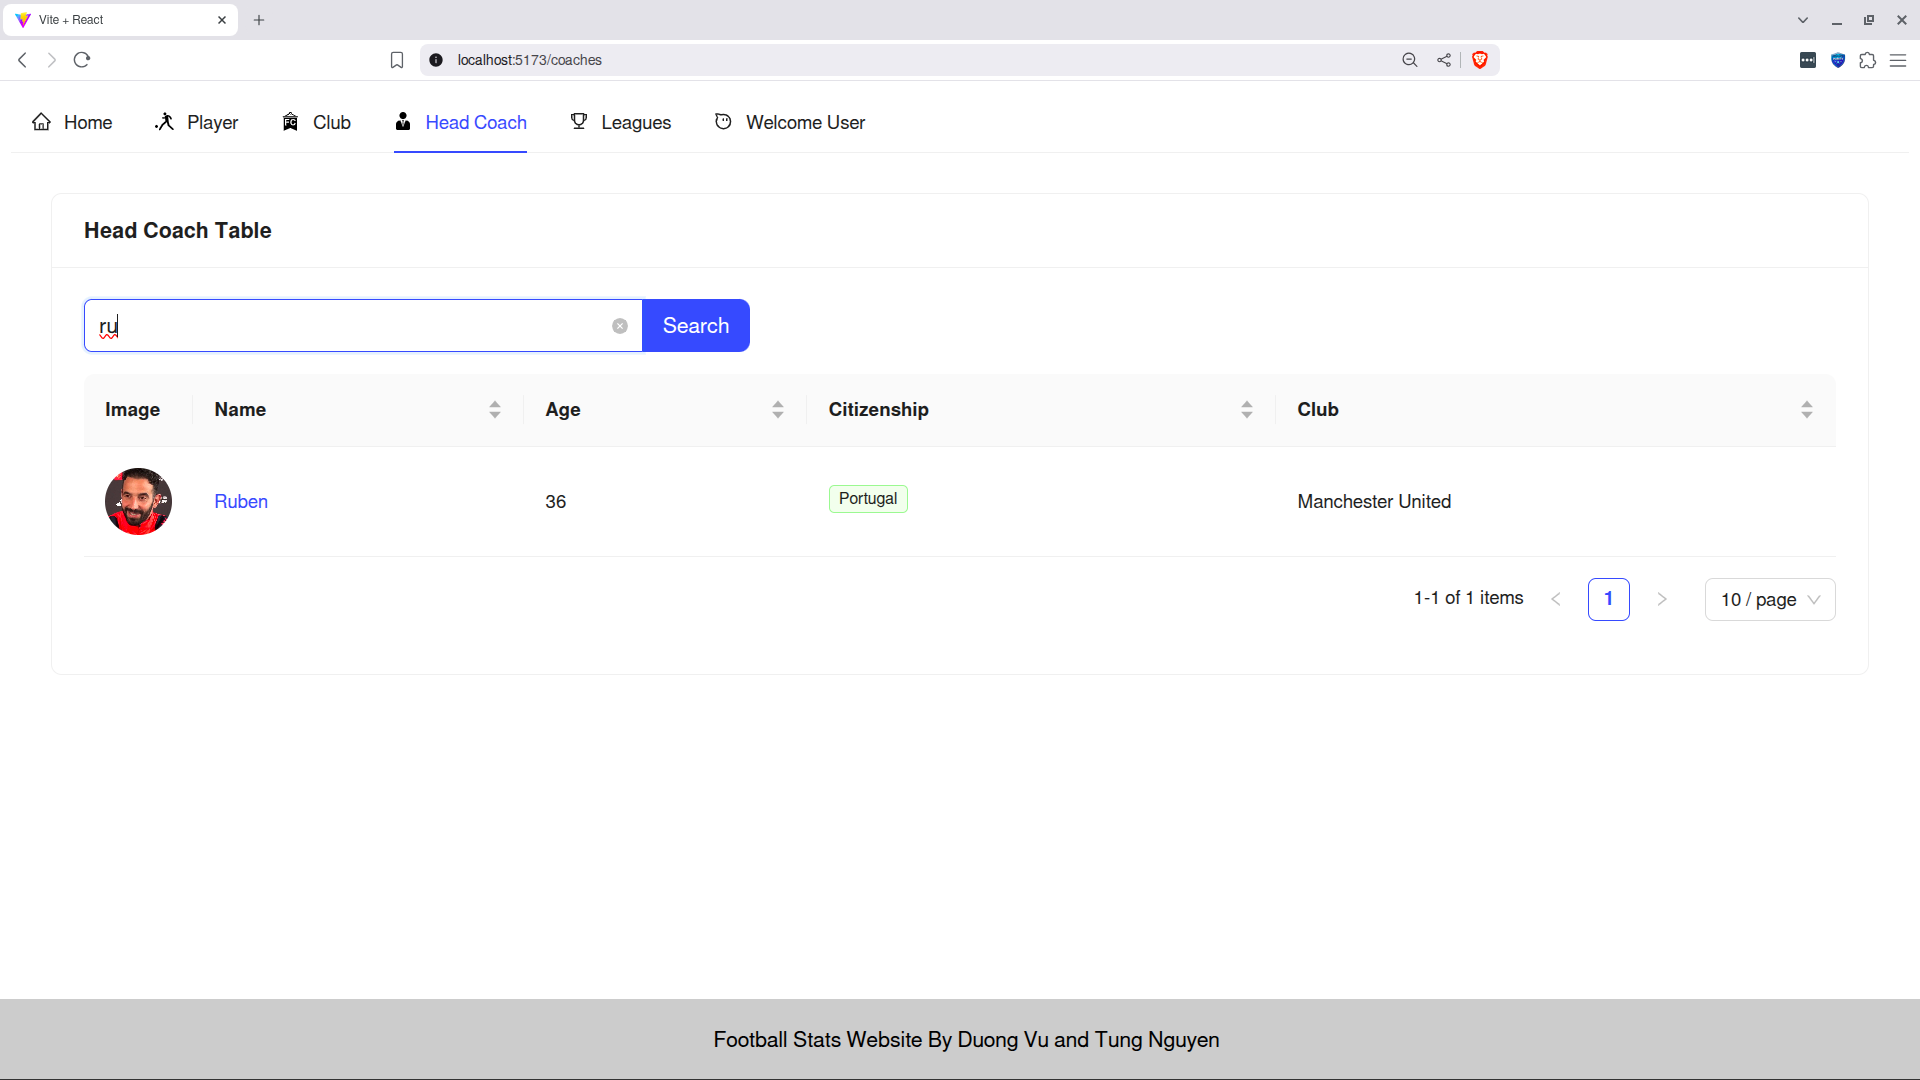
\includegraphics[width=1\linewidth]{Hinhve/user-coach-search.png}
\caption{Giao diện tìm kiếm huấn luyện viên}
\label{fig:user-coach-search}
\end{figure}


\subsubsection{Giao diện lọc huấn luyện viên}
Giao diện lọc huấn luyện viên như trên hình \ref{fig:user-coach-filter}.
\begin{figure}
\centering
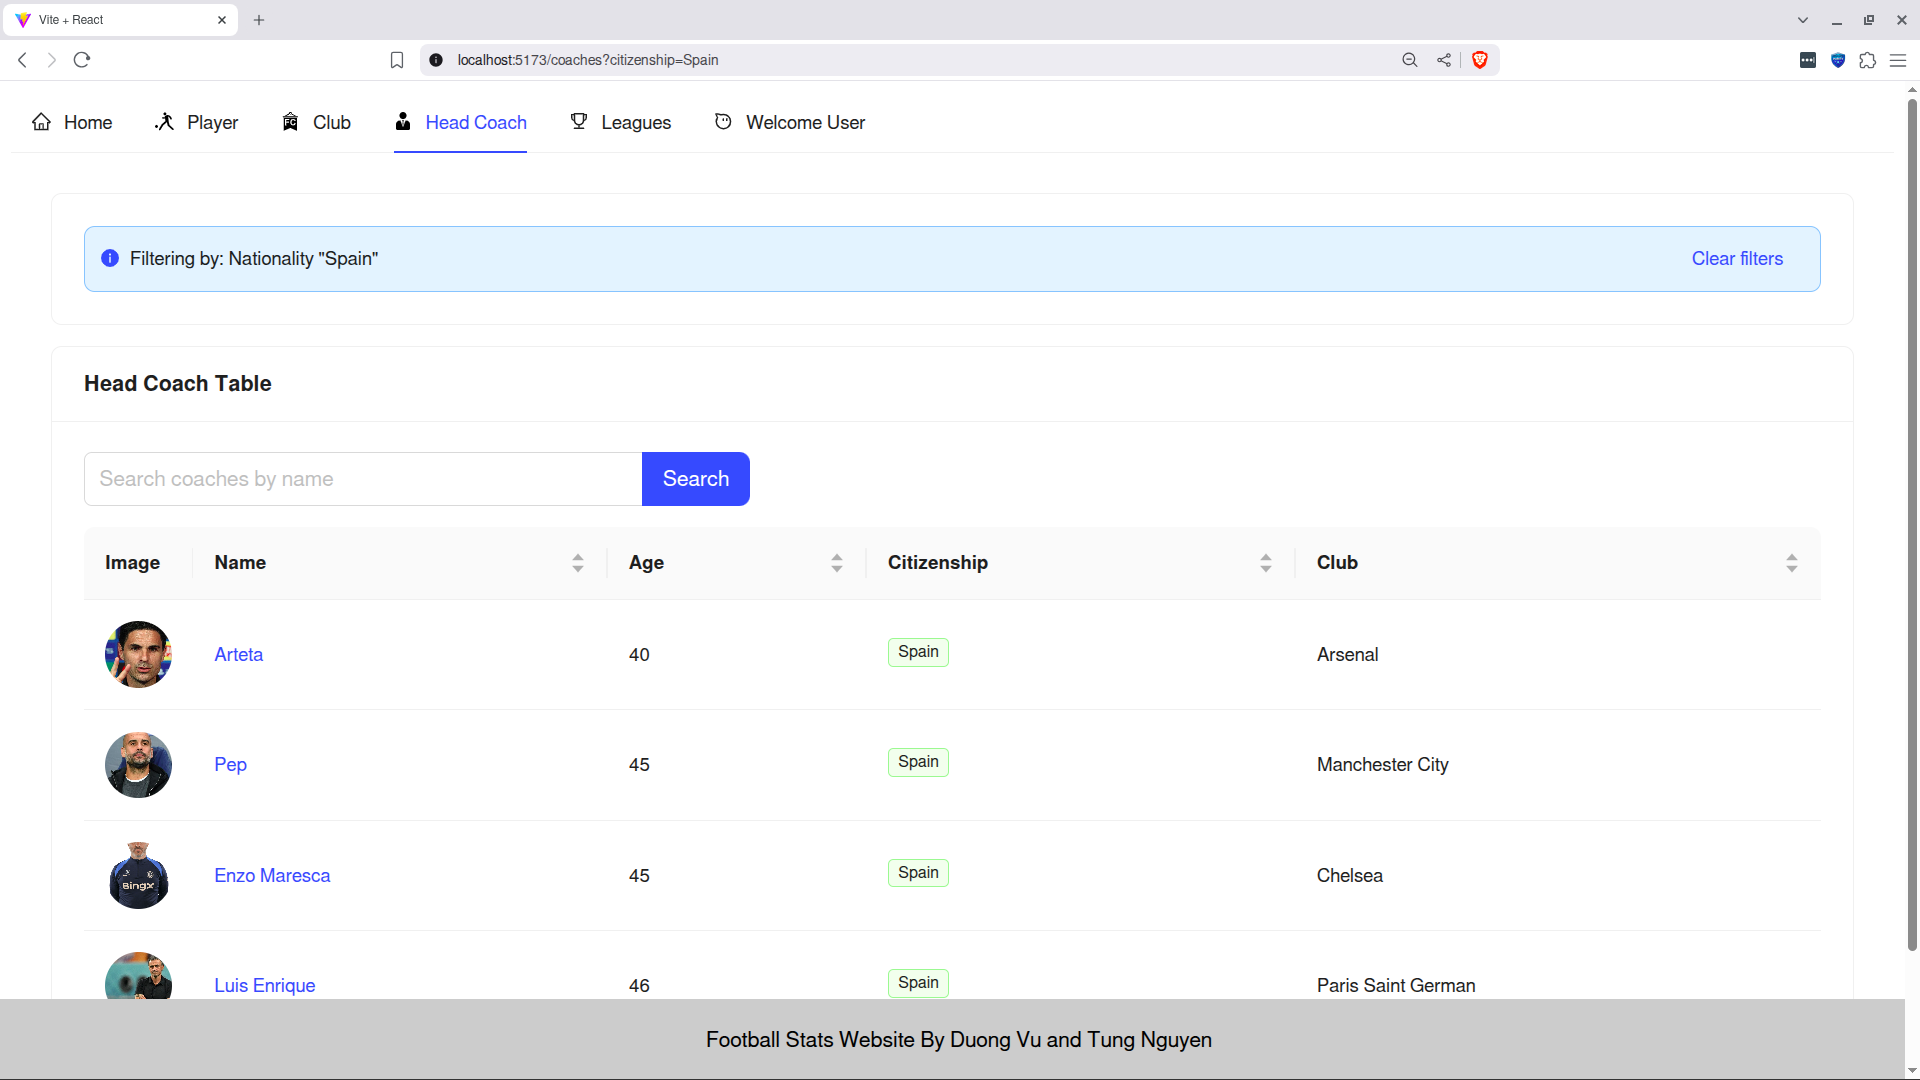
\includegraphics[width=1\linewidth]{Hinhve/user-coach-filter.png}
\caption{Giao diện lọc huấn luyện viên}
\label{fig:user-coach-filter}
\end{figure}

\subsubsection{Giao diện chi tiết huấn luyện viên}
Giao diện chi tiết huấn luyện viên như trên hình \ref{fig:user-coach-detail}.
\begin{figure}
\centering
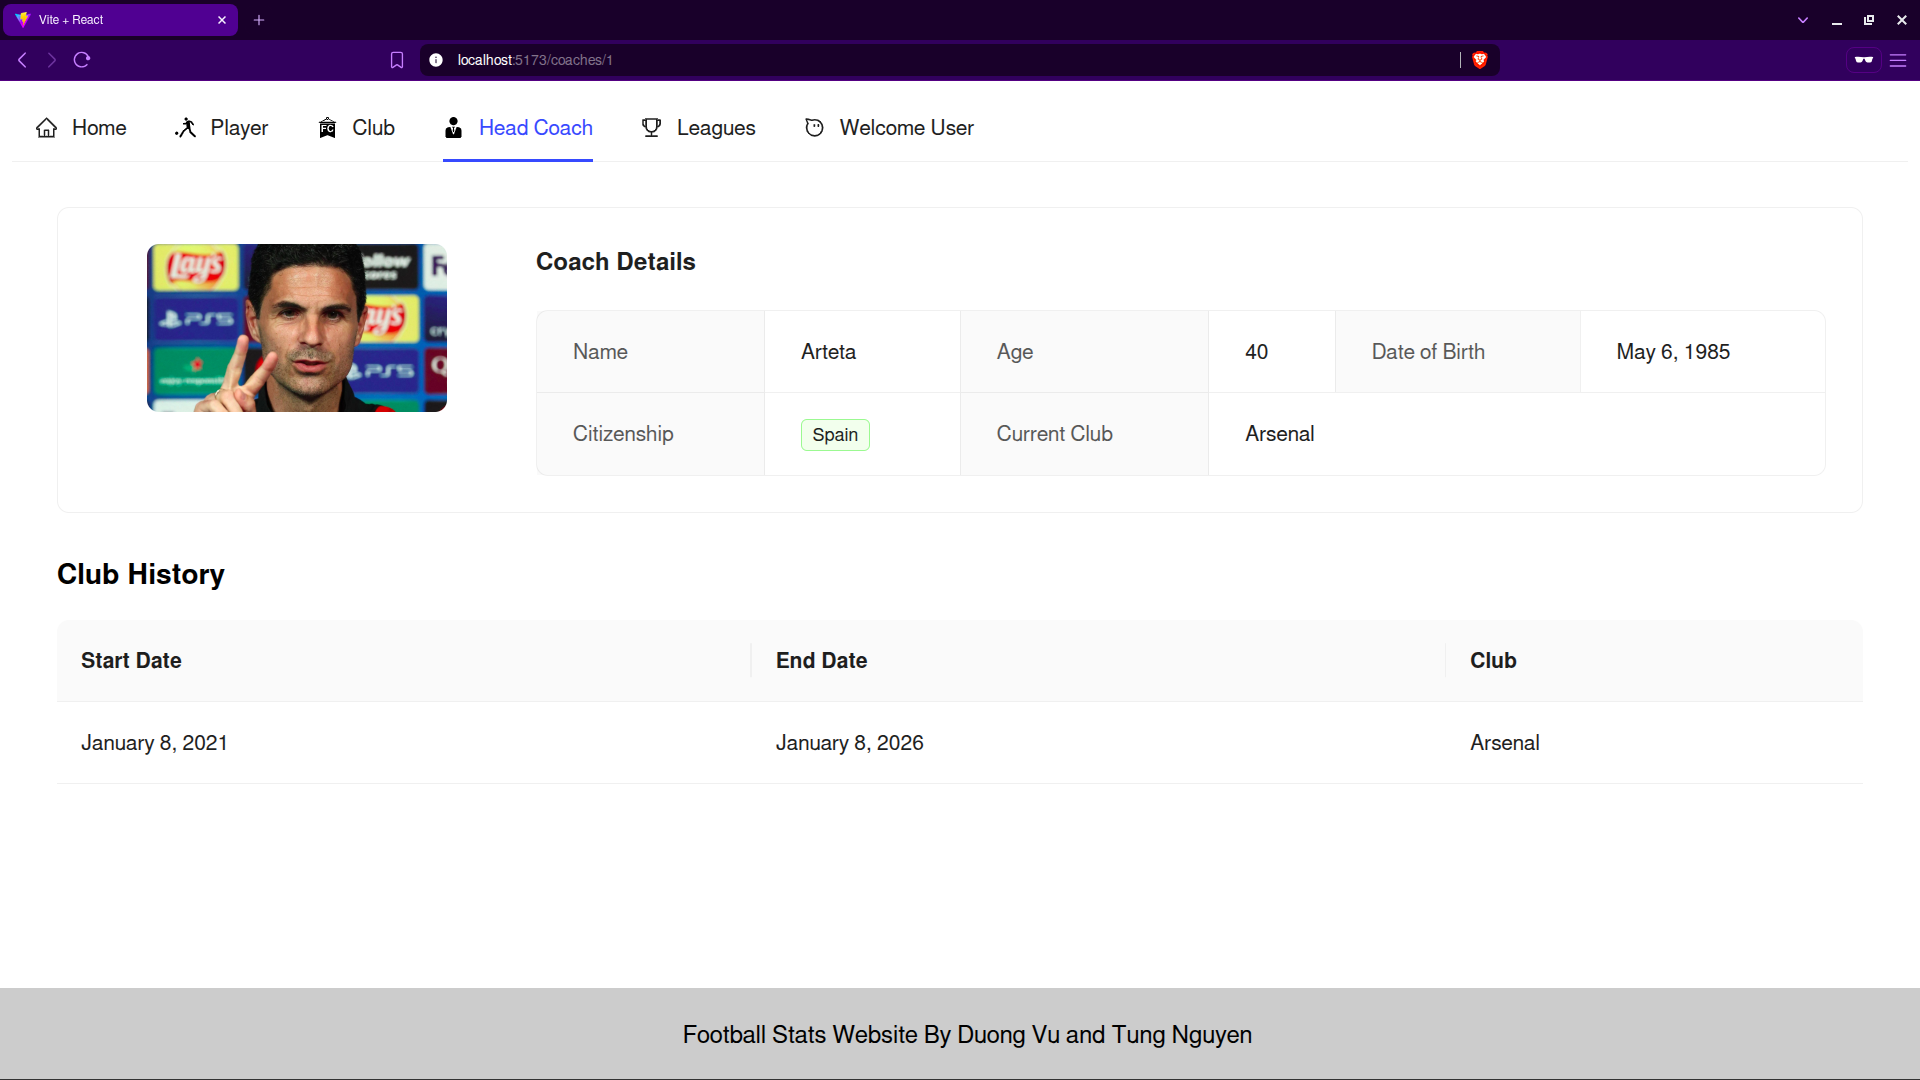
\includegraphics[width=1\linewidth]{Hinhve/user-coach-detail.png}
\caption{Giao diện chi tiết huấn luyện viên}
\label{fig:user-coach-detail}
\end{figure}
\subsection{ Giao diện giải đấu}
\subsubsection{Giao diện danh sách giải đấu}
Giao diện danh sách giải đấu như trên hình \ref{fig:user-league-list}.
\begin{figure}
\centering
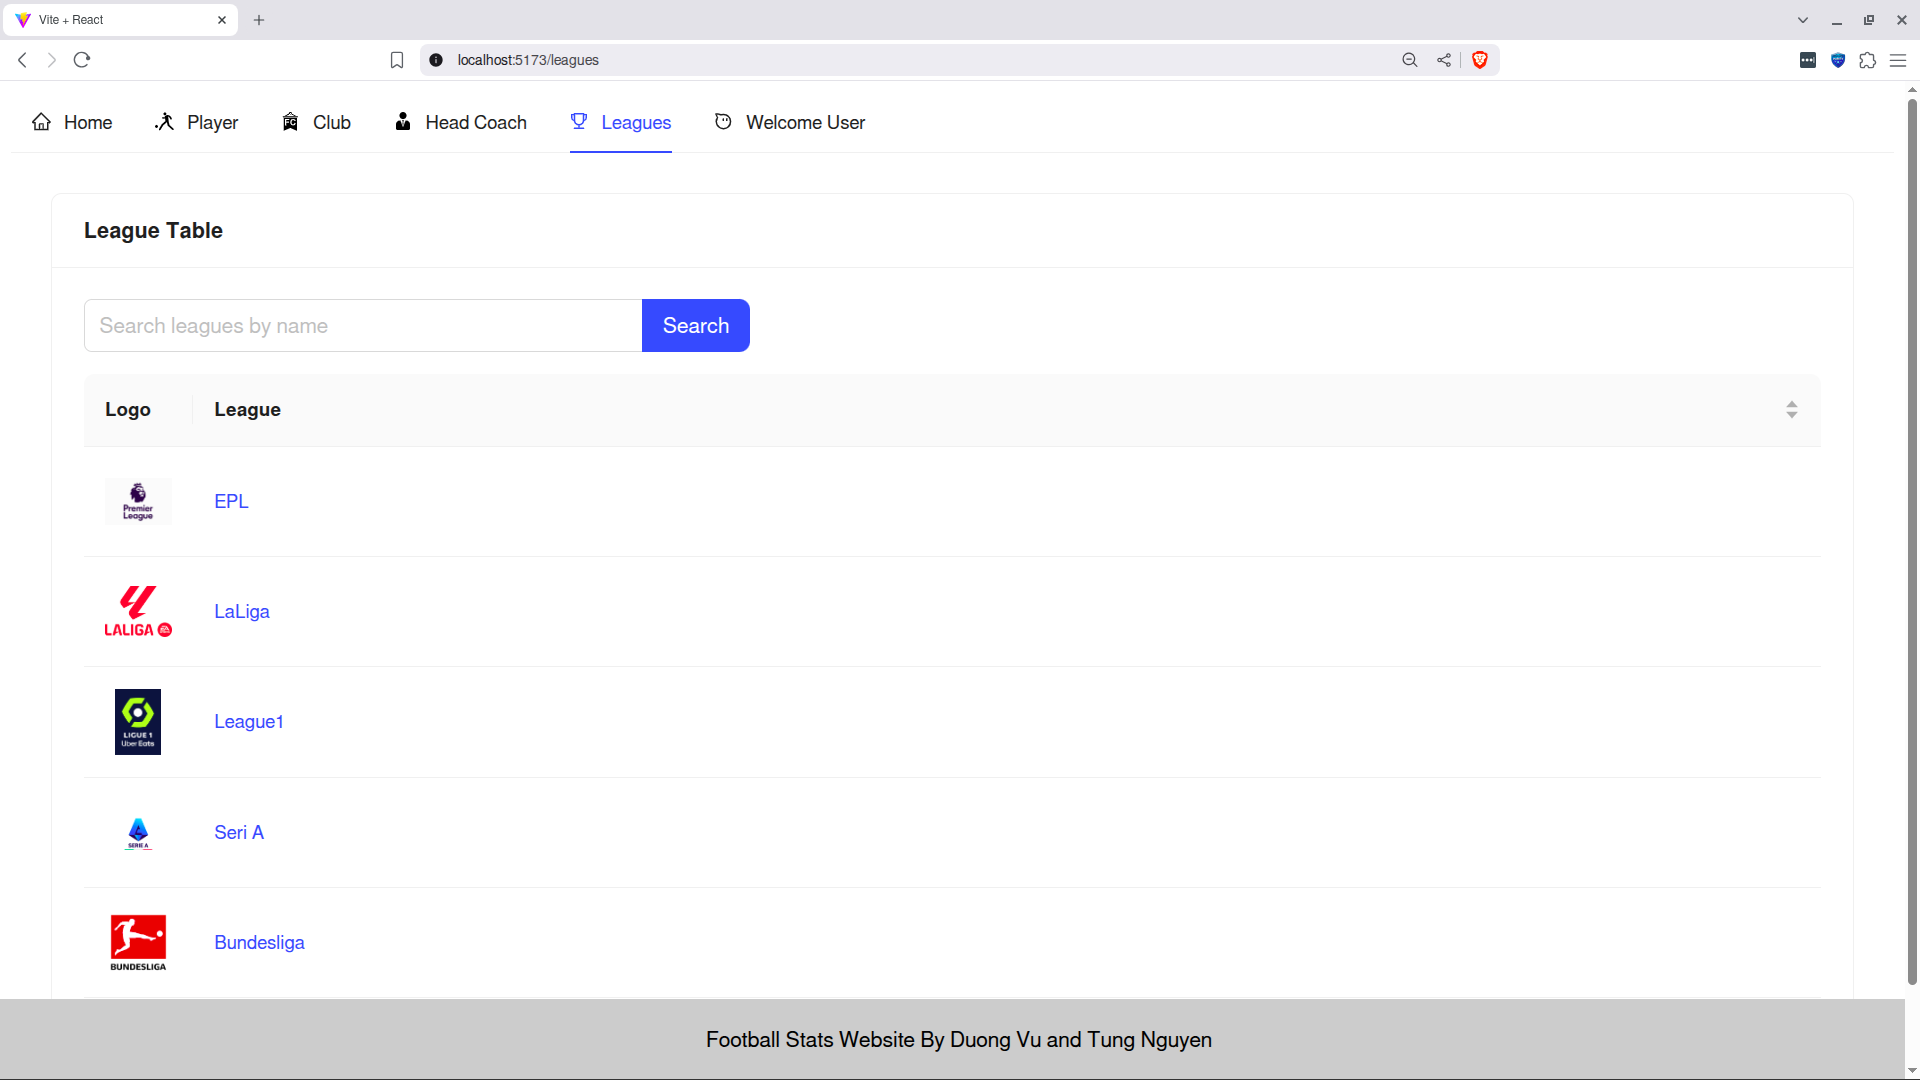
\includegraphics[width=1\linewidth]{Hinhve/user-league-list.png}
\caption{Giao diện danh sách giải đấu}
\label{fig:user-league-list}
\end{figure}

\subsubsection{Giao diện tìm kiếm giải đấu}
Giao diện tìm kiếm giải đấu như trên hình \ref{fig:user-league-search}.
\begin{figure}
\centering
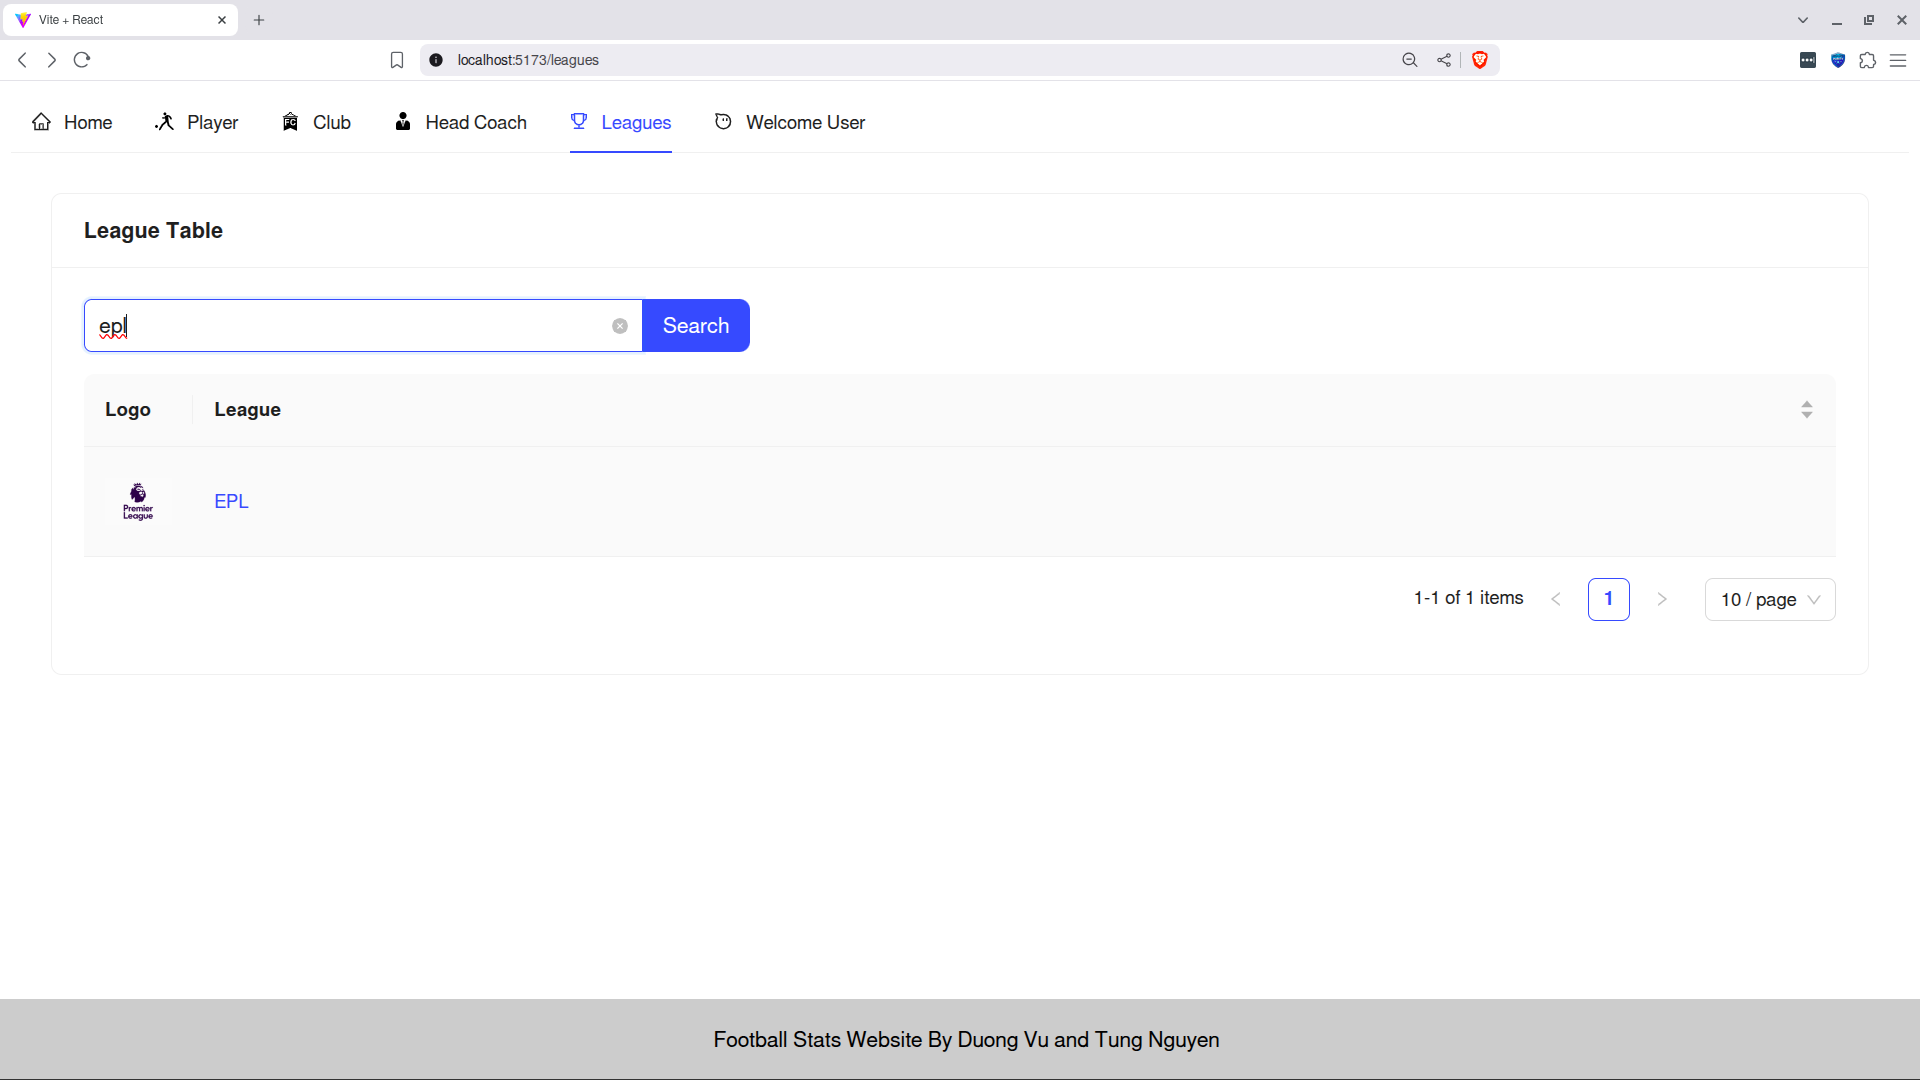
\includegraphics[width=1\linewidth]{Hinhve/user-league-search.png}
\caption{Giao diện tìm kiếm giải đấu}
\label{fig:user-league-search}
\end{figure}
\subsubsection{ Giao diện chi tiết giải đấu}
Giao diện chi tiết giải đấu như trên các hình \ref{fig:user-league-season1}, \ref{fig:user-league-season2}, \ref{fig:user-league-season3}, \ref{fig:user-league-season4}.
\begin{figure}
    \centering
    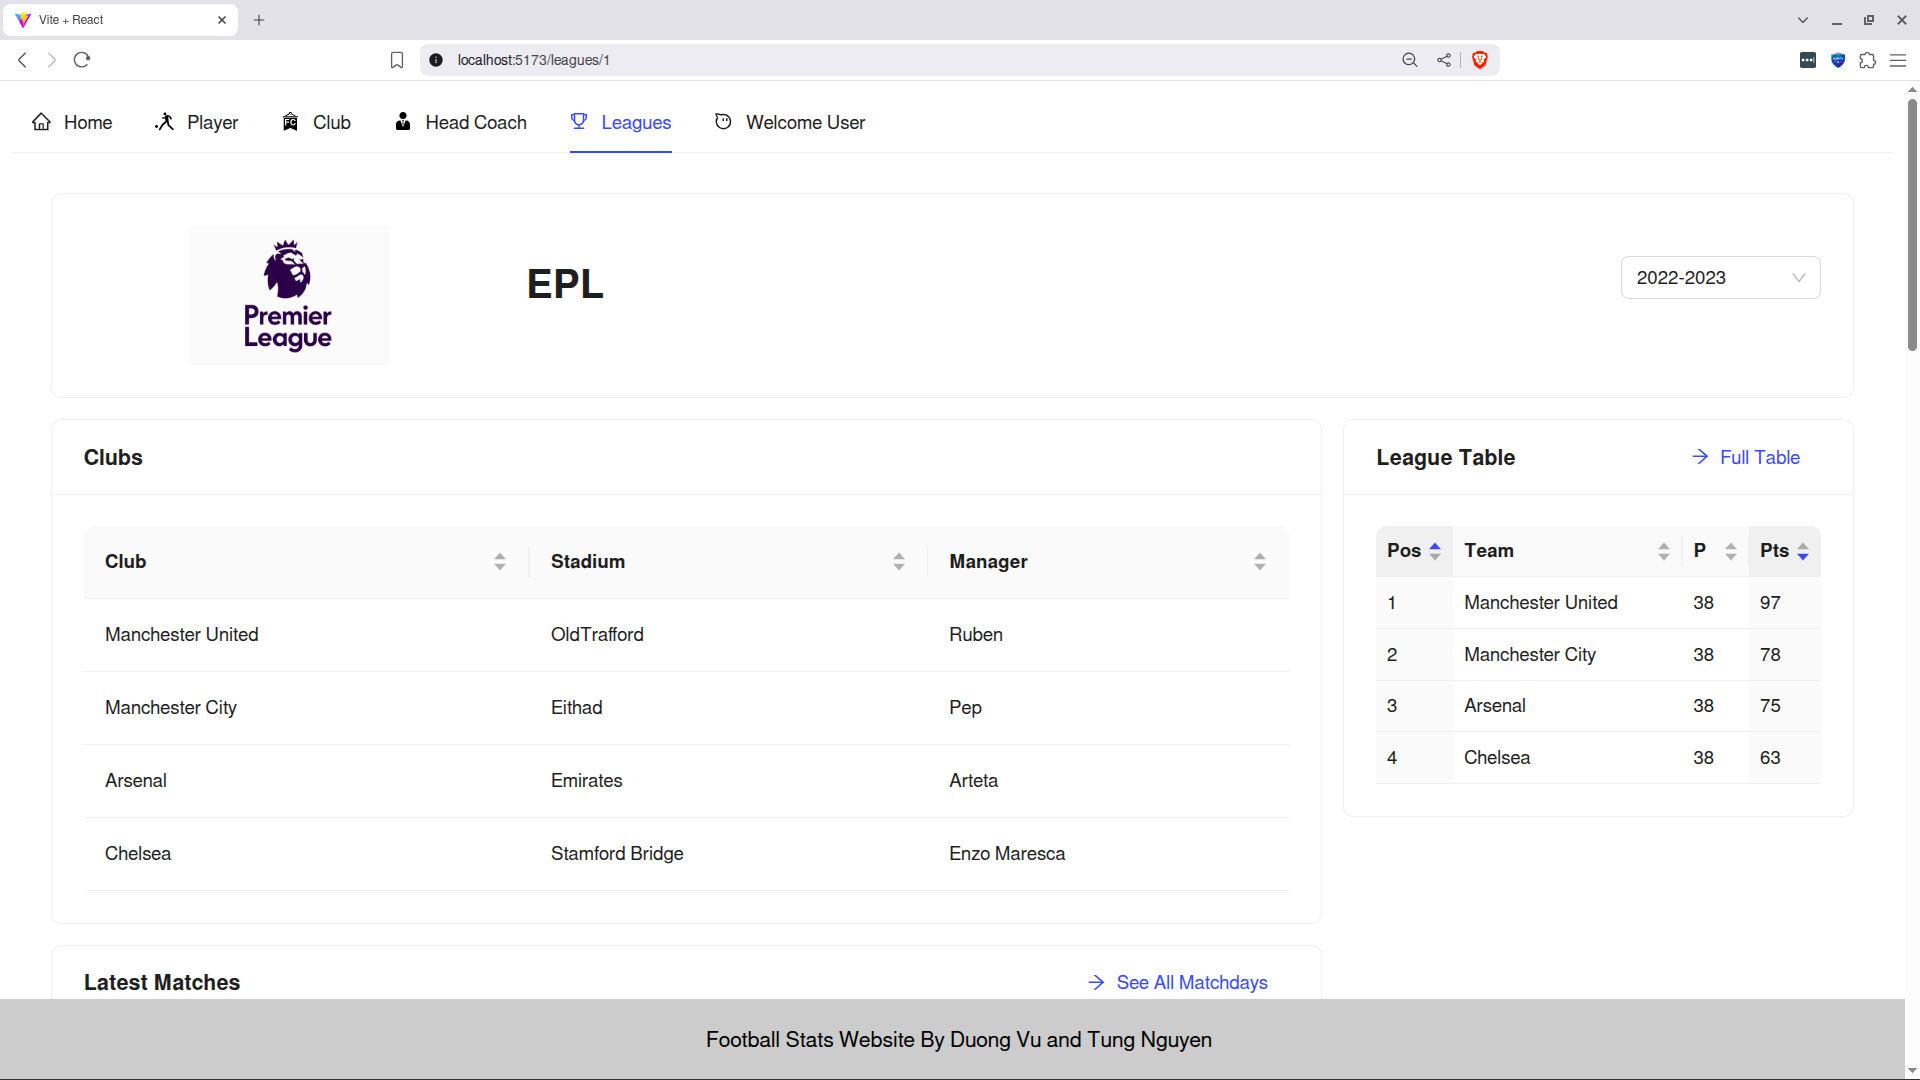
\includegraphics[width=1\linewidth]{Hinhve/user-league-season1.png}
    \caption{ Giao diện chi tiết giải đấu - ảnh 1}
    \label{fig:user-league-season1}
\end{figure}
\begin{figure}
    \centering
    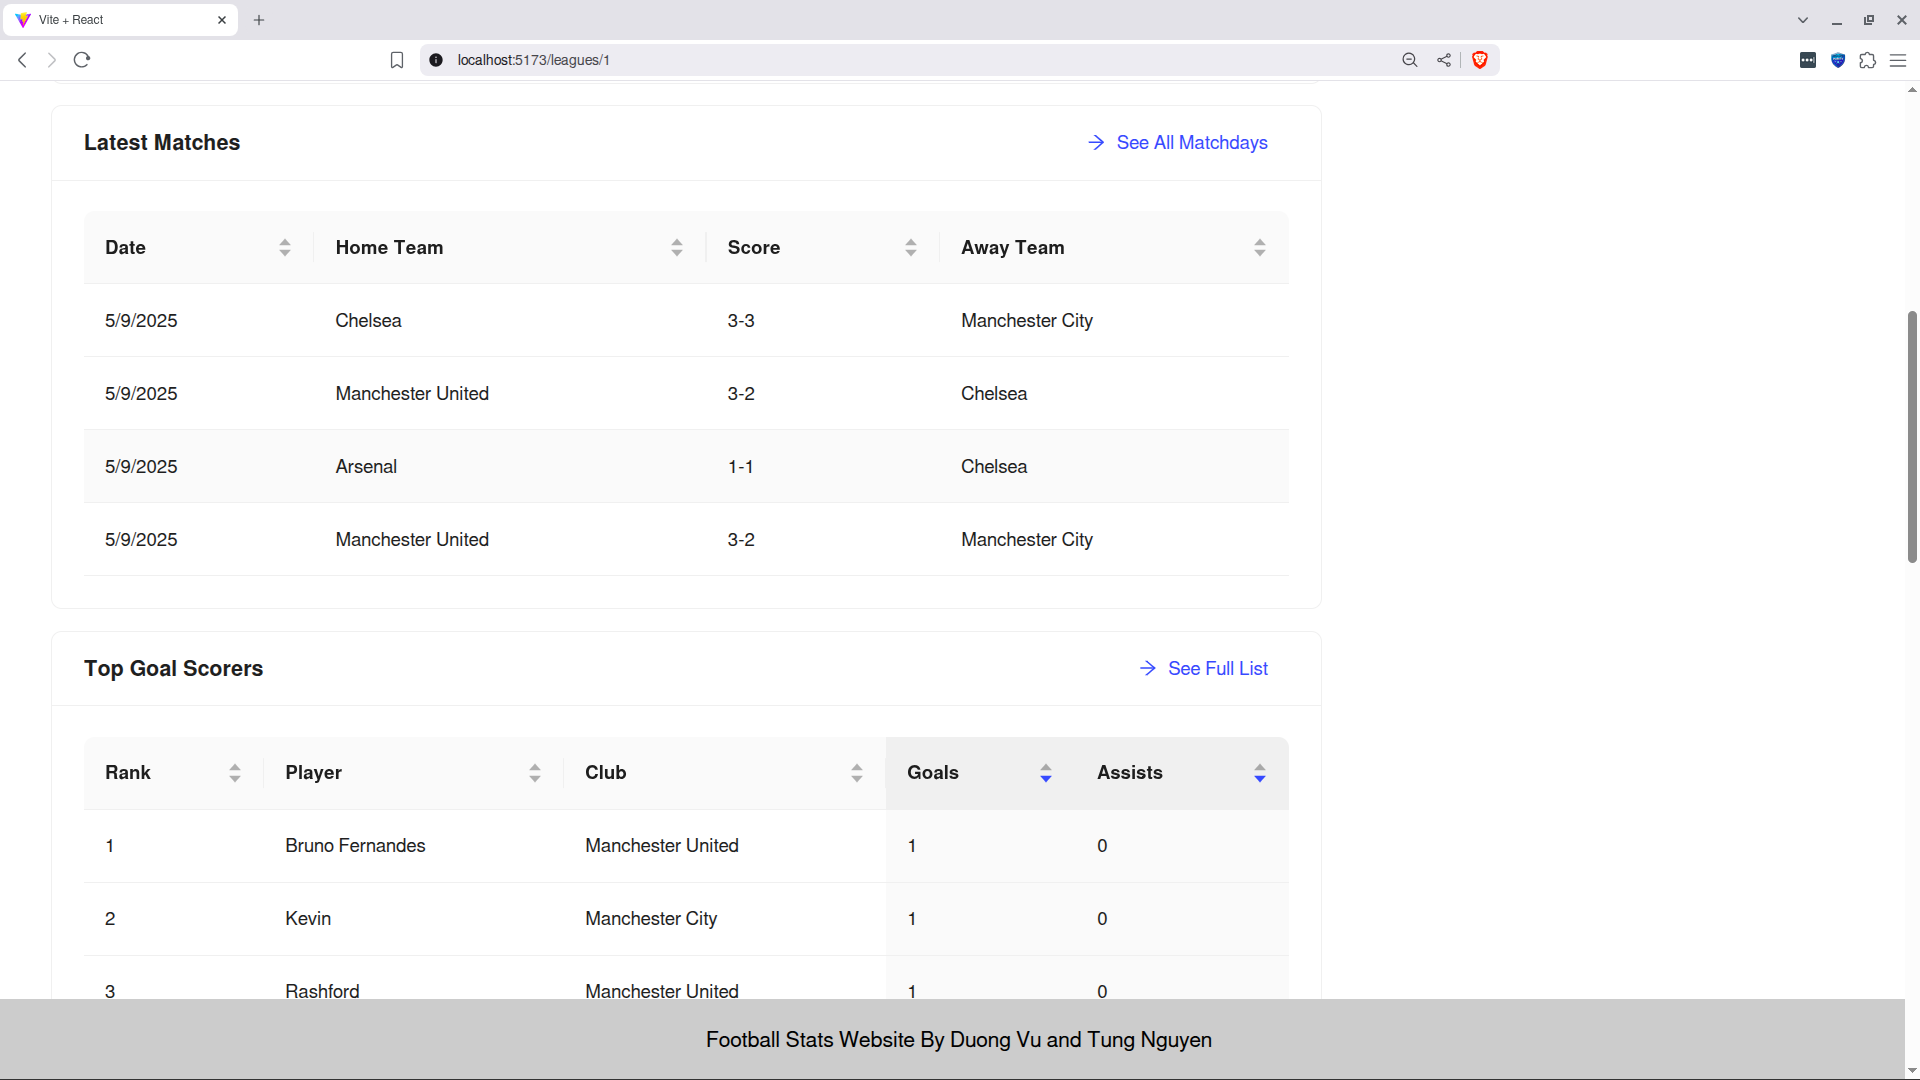
\includegraphics[width=1\linewidth]{Hinhve/user-league-season2.png}
    \caption{ Giao diện chi tiết giải đấu - ảnh 2}
    \label{fig:user-league-season2}
\end{figure}
\begin{figure}
    \centering
    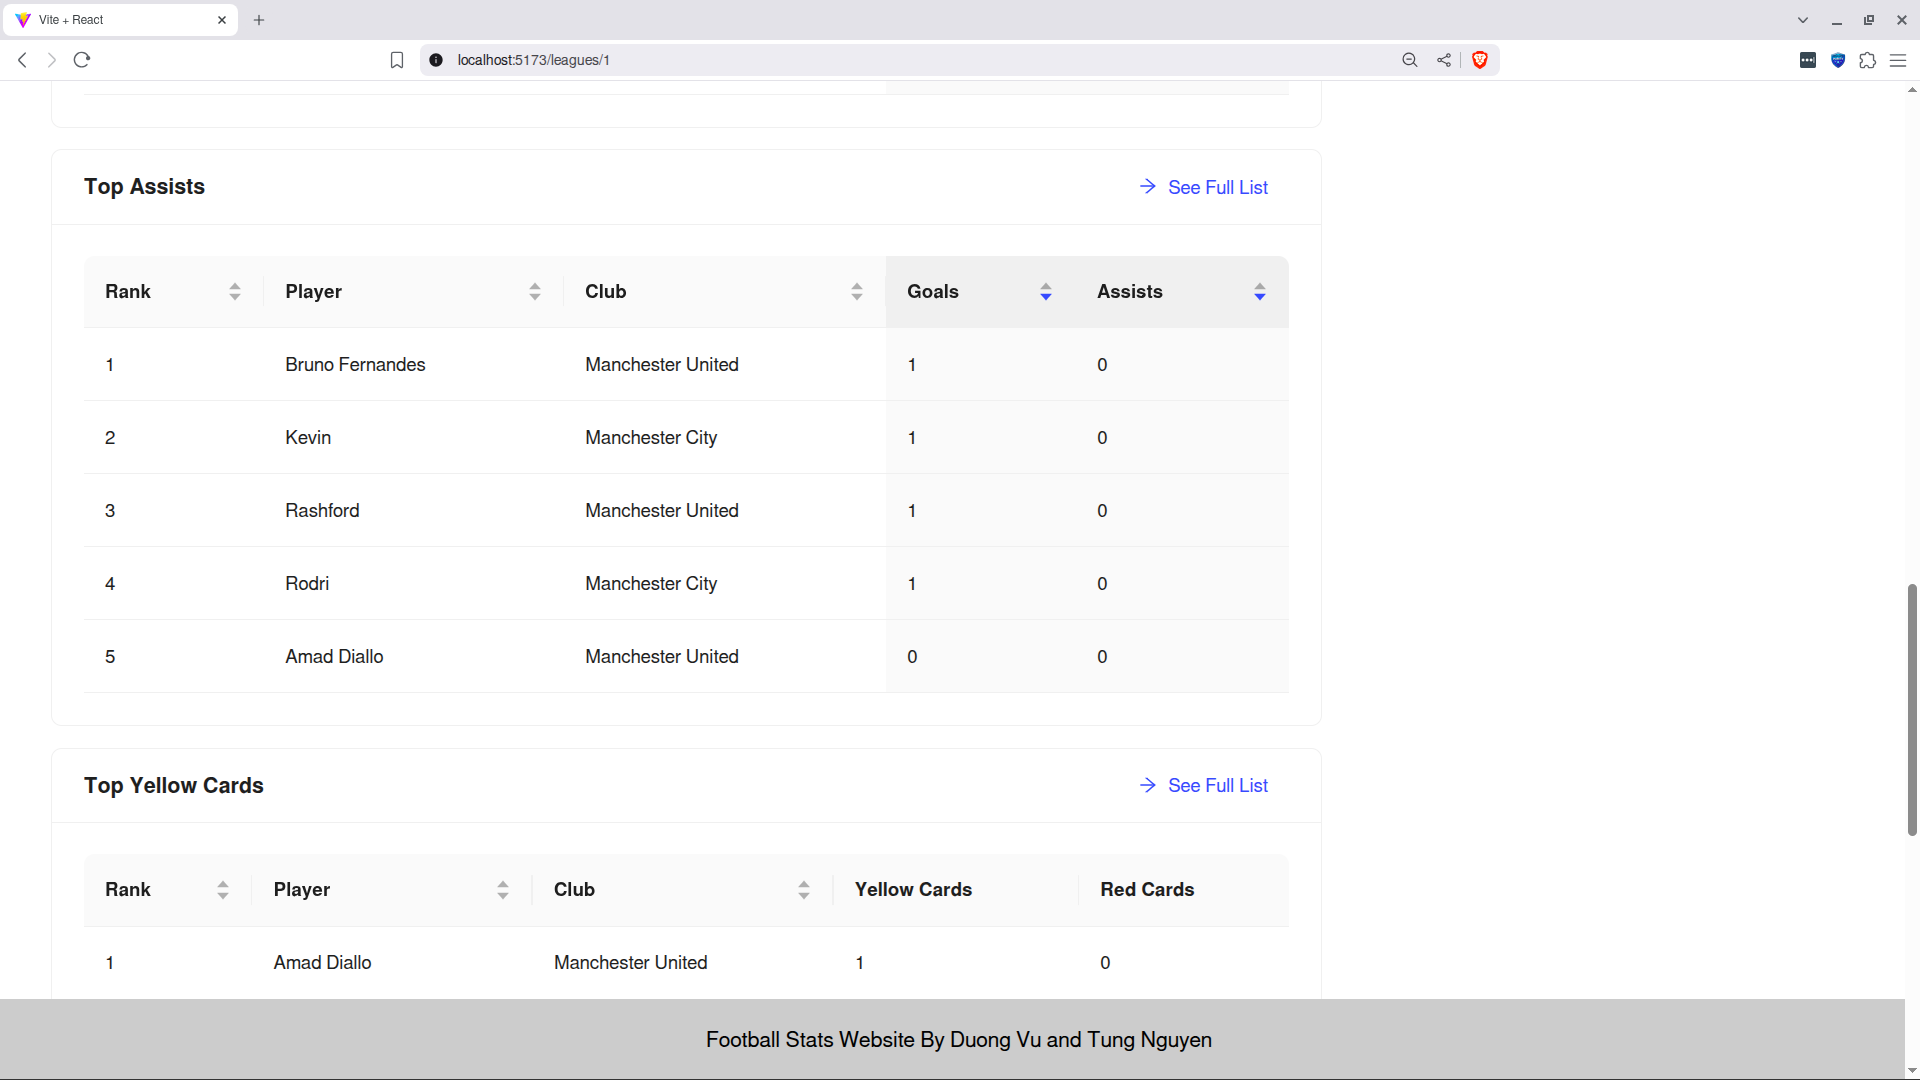
\includegraphics[width=1\linewidth]{Hinhve/user-league-season3.png}
    \caption{ Giao diện chi tiết giải đấu - ảnh 3}
    \label{fig:user-league-season3}
\end{figure}
\begin{figure}
    \centering
    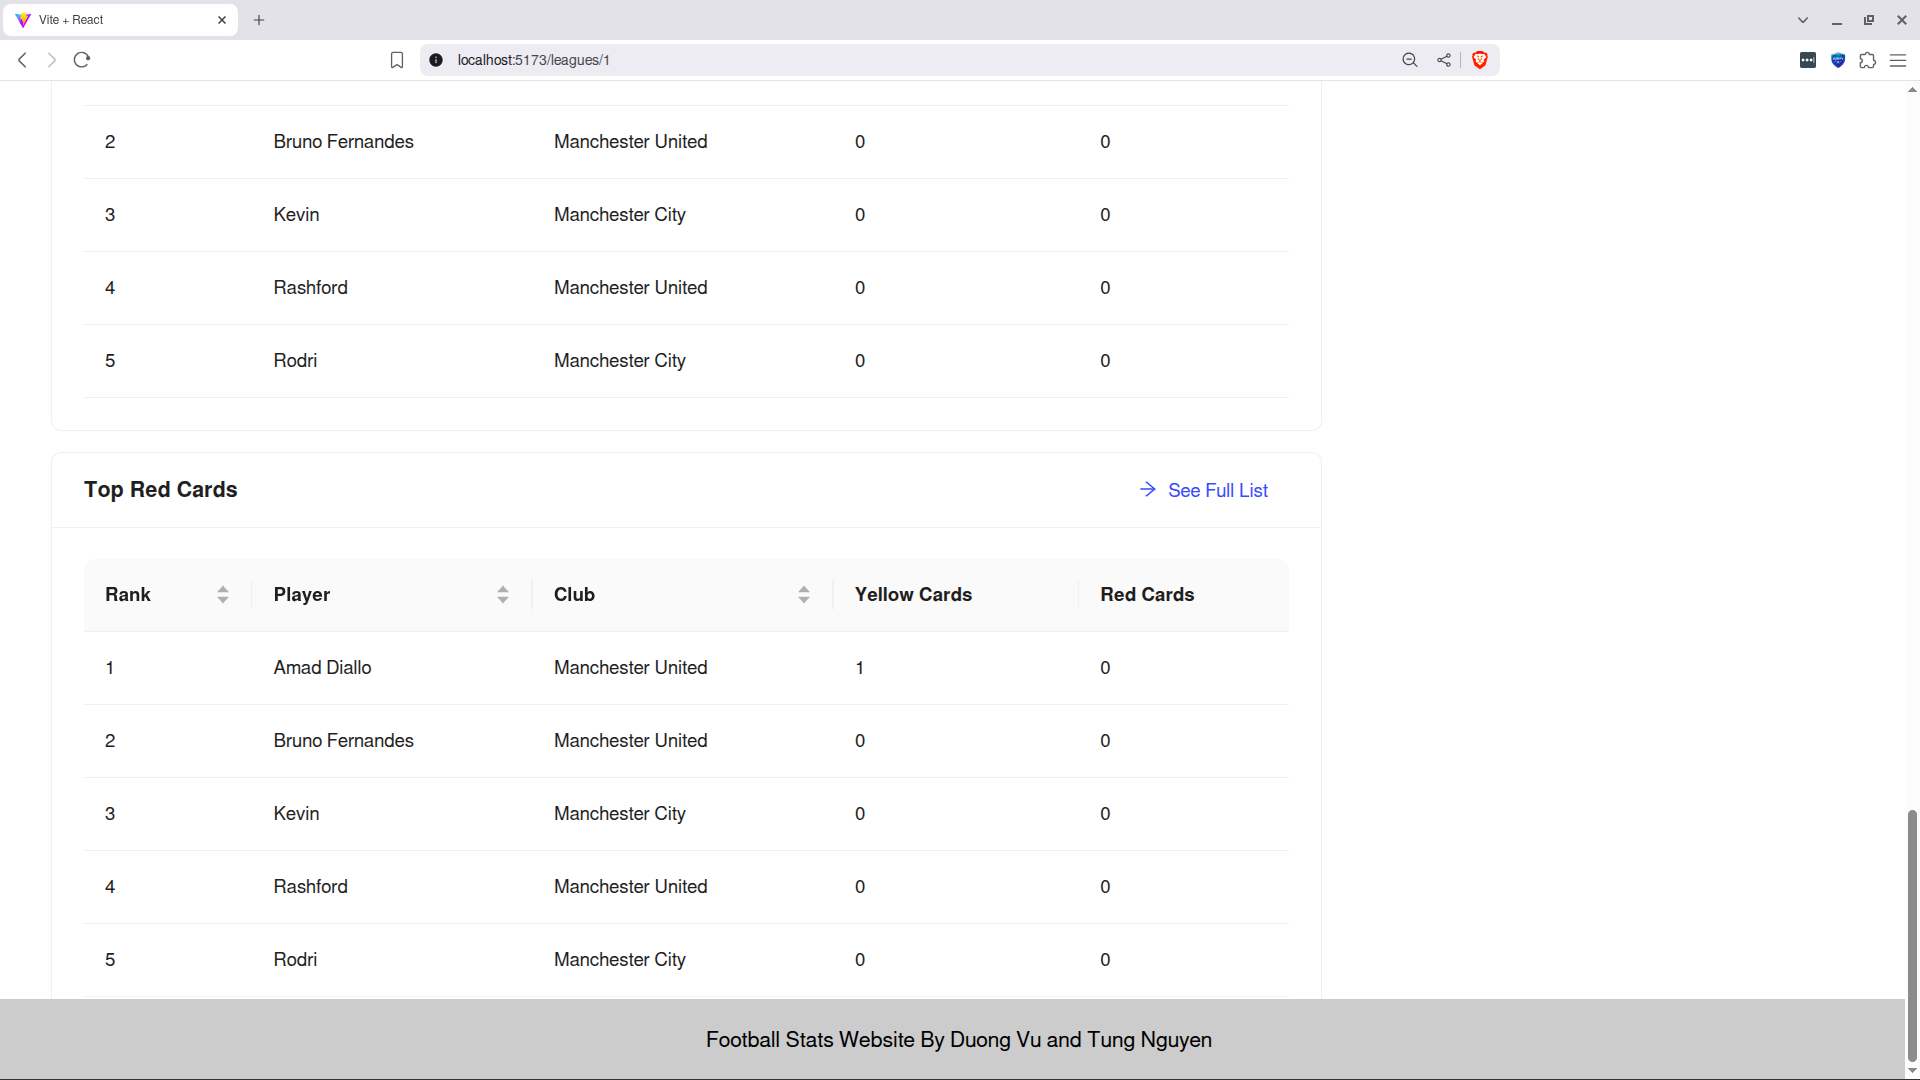
\includegraphics[width=1\linewidth]{Hinhve/user-league-season4.png}
    \caption{ Giao diện chi tiết giải đấu - ảnh 4}
    \label{fig:user-league-season4}
\end{figure}
\section{ Giao diện Admin}
\subsection{Giao diện tìm kiếm trang chủ}
\begin{figure}
    \centering
    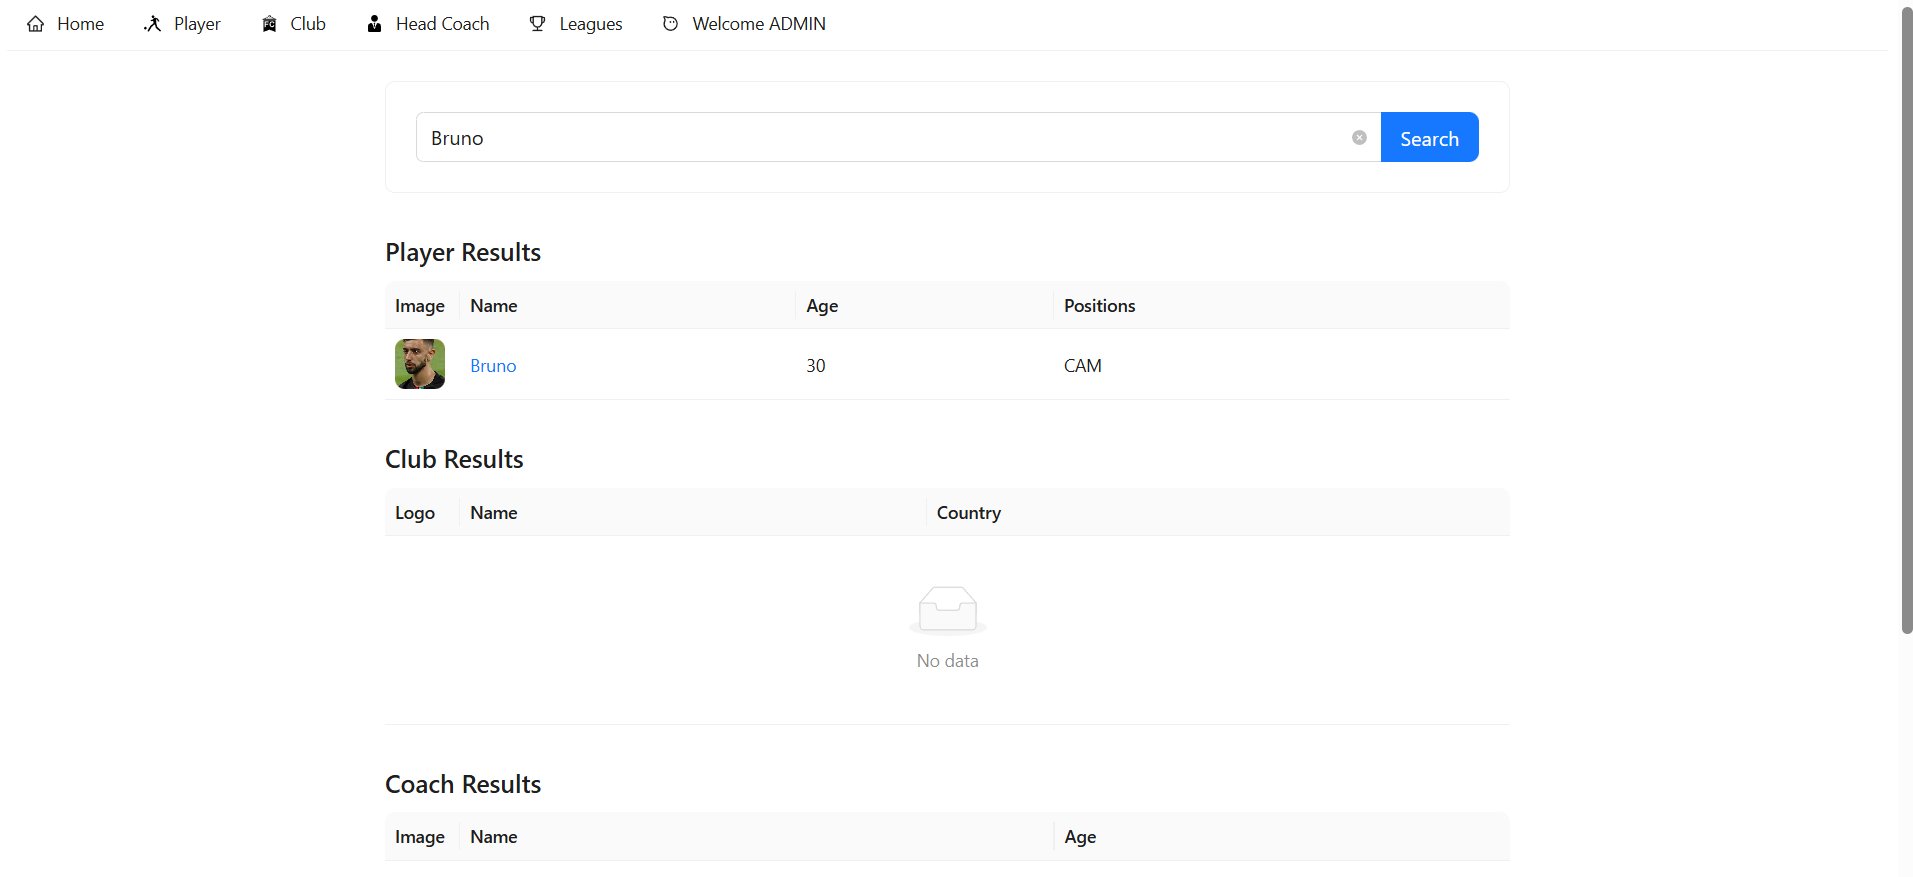
\includegraphics[width=1\linewidth]{Hinhve/search_home.png}
    \caption{Giao diện tìm kiếm cho admin}
    \label{fig:search_home}
\end{figure}
Giao diện tìm kiếm trang chủ như trên hình \ref{fig:search_home}. Admin có thể nhập tên cầu thủ, câu lạc bộ, giải đấu, huấn luyện viên,... để tìm kiếm, hệ thống sẽ hiển thị kết quả tương ứng.

\subsection{Giao diện hiển thị cầu thủ}
\begin{figure}
    \centering
    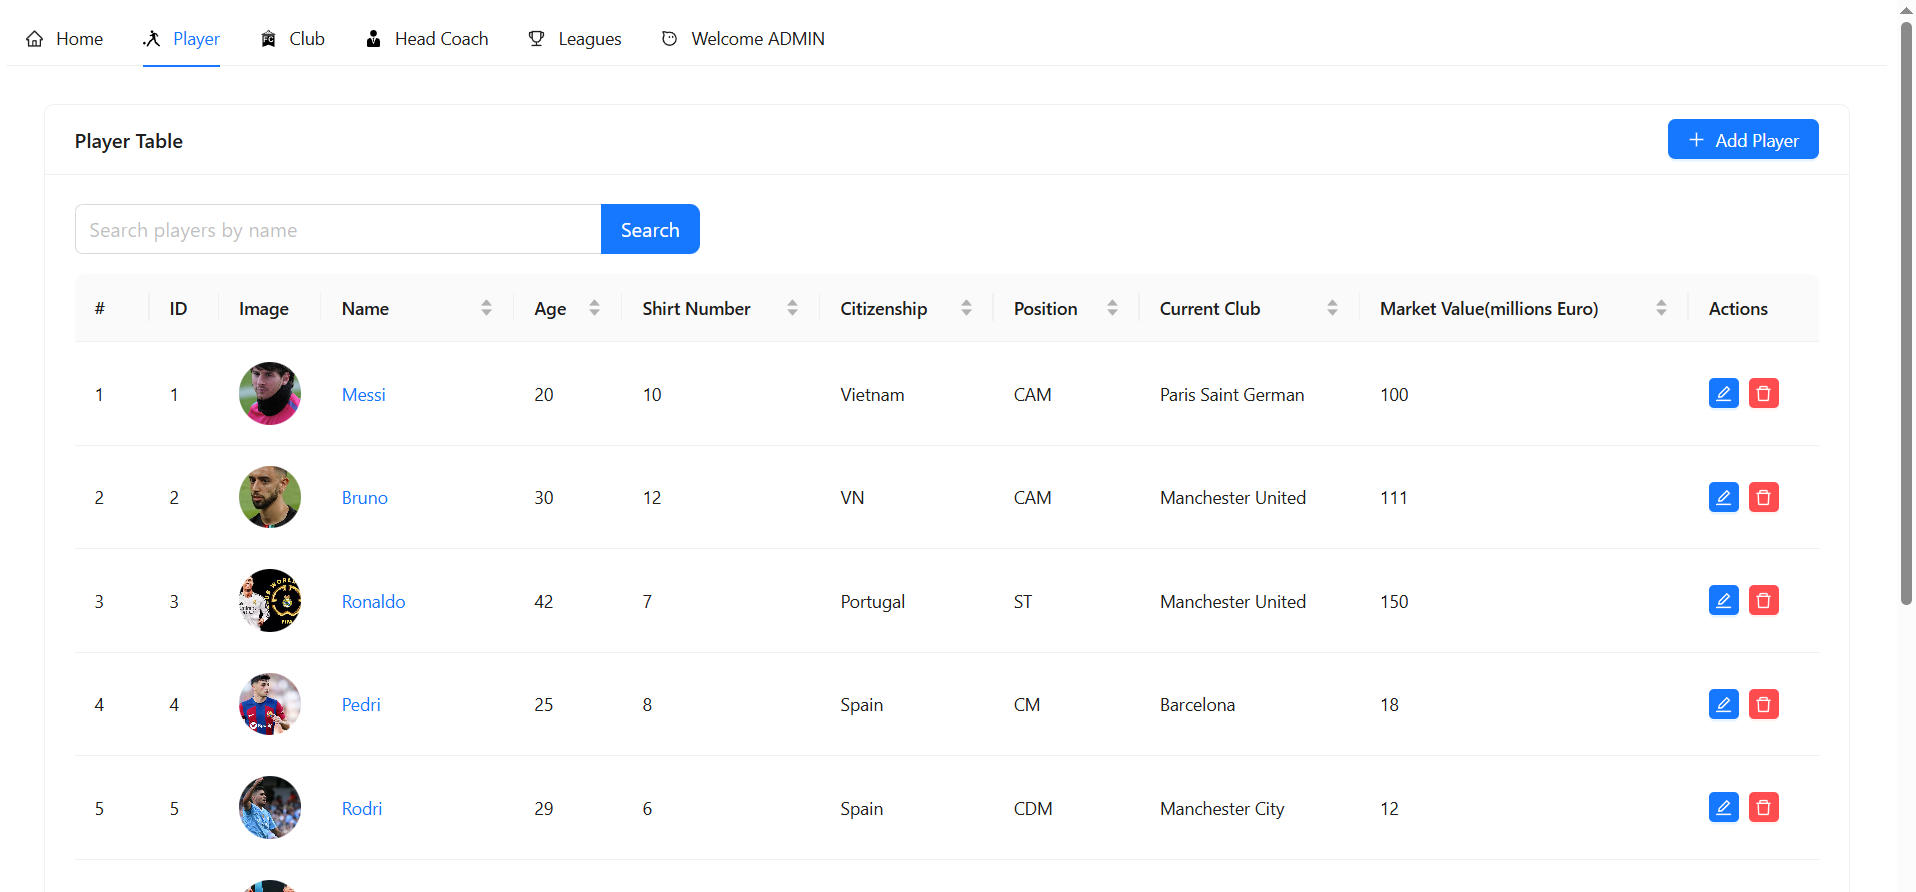
\includegraphics[width=1\linewidth]{Hinhve/admin_players.png}
    \caption{Giao diện hiển thị cầu thủ}
    \label{fig:admin_players}
\end{figure}
Giao diện hiển thị cầu thủ như trên hình \ref{fig:admin_players}. Giao diện này hiển thị danh sách tất cả cầu thủ hiện có trong cơ sở dữ liệu.

\subsection{Giao diện tìm kiếm cầu thủ}
\begin{figure}
    \centering
    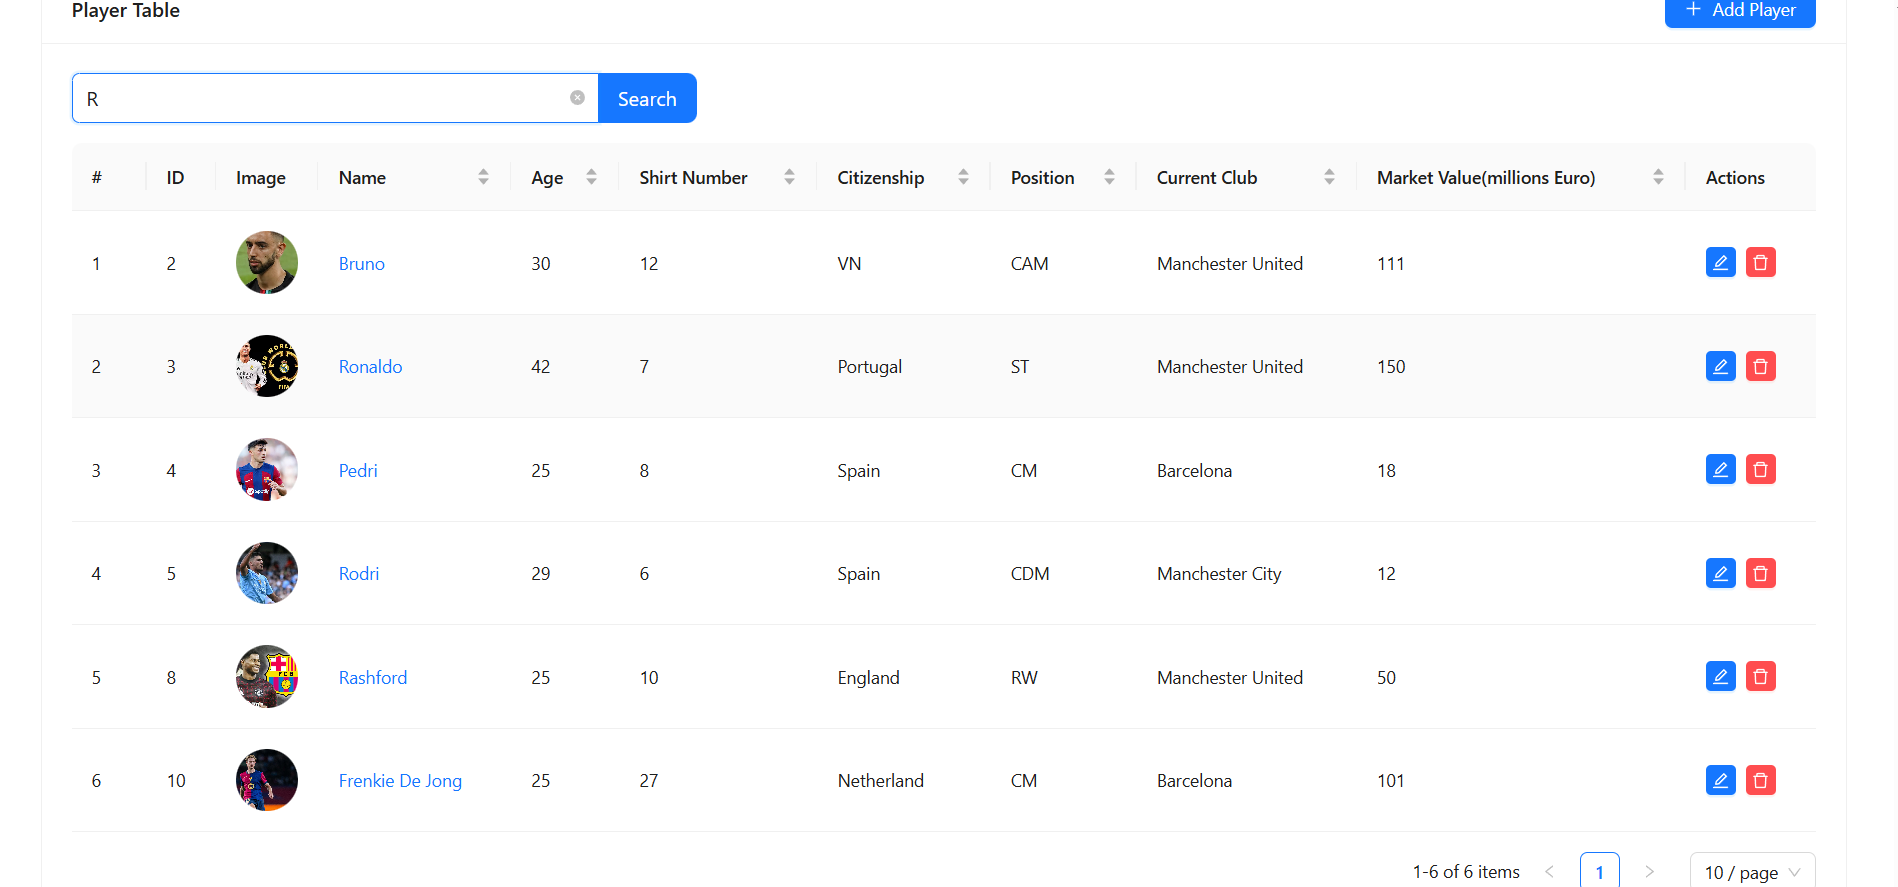
\includegraphics[width=1\linewidth]{Hinhve/admin_search_player.png}
    \caption{Giao diện tìm kiếm cầu thủ}
    \label{fig:admin_search_player}
\end{figure}
Giao diện tìm kiếm cầu thủ như trên hình \ref{fig:admin_search_player}. Admin nhập tên vào thanh tìm kiếm để lọc ra các cầu thủ theo tên.

\subsection{Giao diện thêm mới cầu thủ}
\begin{figure}
    \centering
    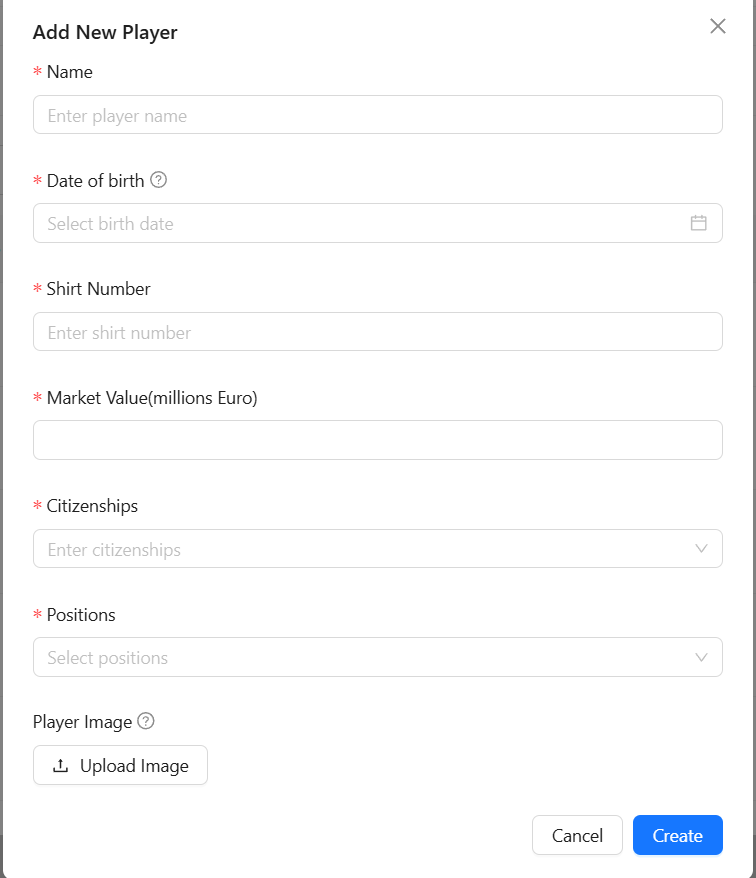
\includegraphics[width=1\linewidth]{Hinhve/admin_add_player.png}
    \caption{Giao diện thêm mới cầu thủ}
    \label{fig:admin_add_player}
\end{figure}
Giao diện thêm mới cầu thủ như trên hình \ref{fig:admin_add_player}. Admin có thể thêm cầu thủ với các thông tin như tên, tuổi, quốc gia, số áo, hình ảnh,...

\subsection{Giao diện chỉnh sửa thông tin cầu thủ}
\begin{figure}
    \centering
    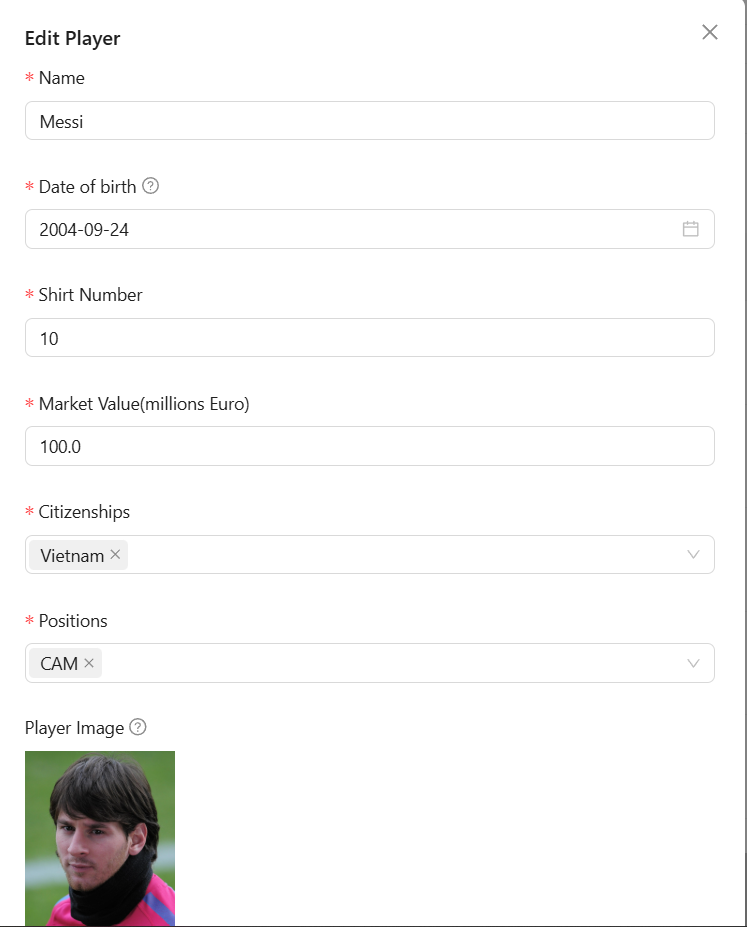
\includegraphics[width=1\linewidth]{Hinhve/admin_edit_player.png}
    \caption{Giao diện chỉnh sửa thông tin cầu thủ}
    \label{fig:admin_edit_player}
\end{figure}
Giao diện chỉnh sửa cầu thủ như trên hình \ref{fig:admin_edit_player}. Admin có thể cập nhật lại thông tin của cầu thủ bao gồm tên, tuổi, quốc gia, số áo, ảnh,...

\subsection{Giao diện chi tiết cầu thủ}
\begin{figure}
    \centering
    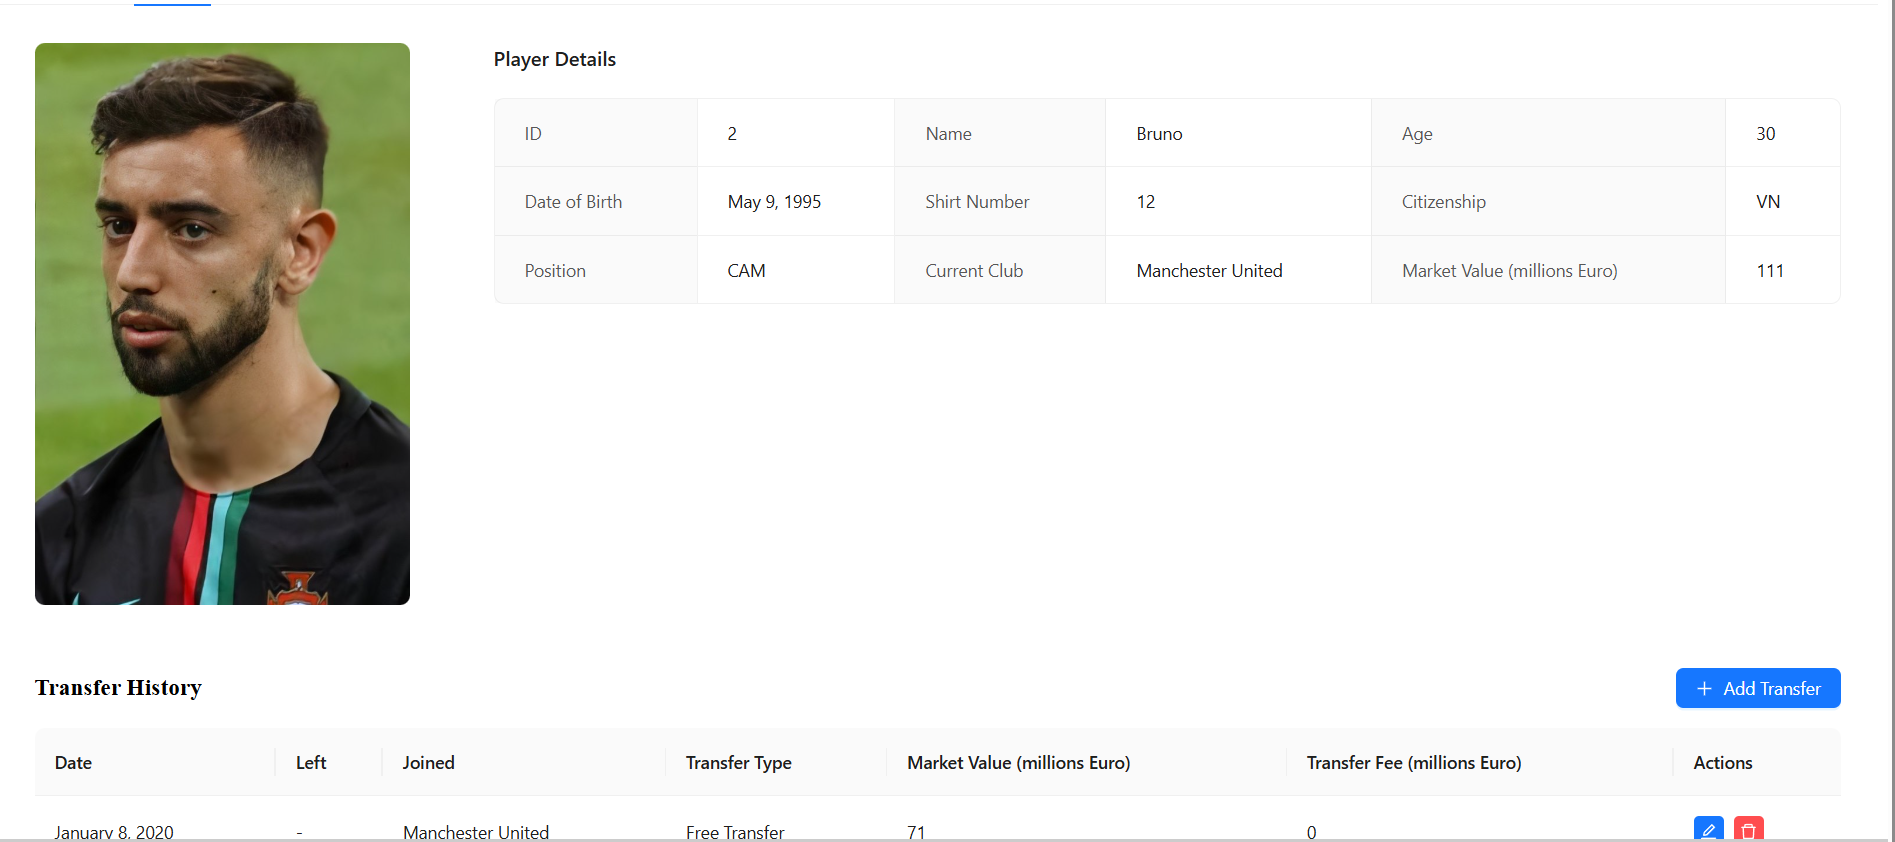
\includegraphics[width=1\linewidth]{Hinhve/admin_player_detail.png}
    \caption{Giao diện chi tiết cầu thủ}
    \label{fig:admin_player_detail}
\end{figure}
Giao diện chi tiết cầu thủ như trên hình \ref{fig:admin_player_detail}. Tất cả thông tin chi tiết về cầu thủ và lịch sử chuyển nhượng sẽ được hiển thị tại đây.

\subsection{Giao diện thêm mới lịch sử chuyển nhượng}
\begin{figure}
    \centering
    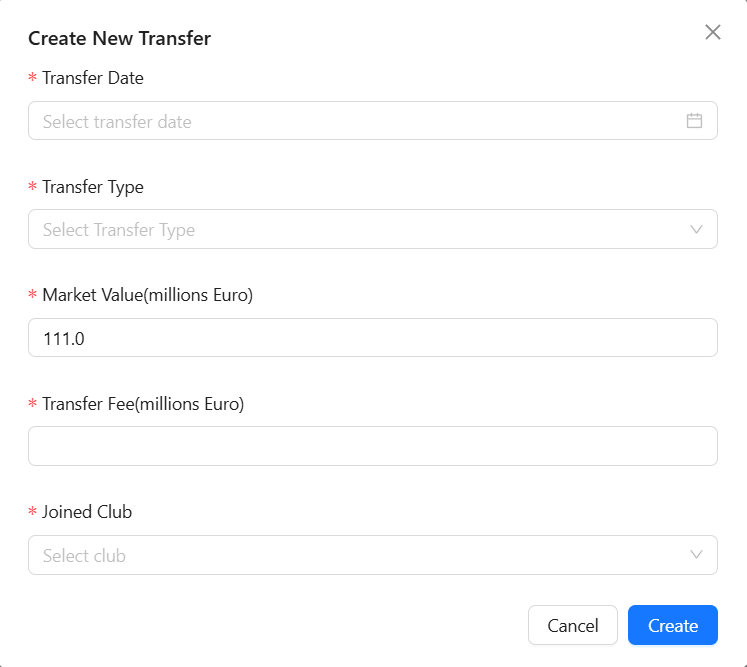
\includegraphics[width=1\linewidth]{Hinhve/admin_add_transfer.png}
    \caption{Giao diện thêm mới lịch sử chuyển nhượng}
    \label{fig:admin_add_transfer}
\end{figure}
Giao diện thêm mới chuyển nhượng như trên hình \ref{fig:admin_add_transfer}. Admin có thể thêm các thông tin chuyển nhượng cho cầu thủ, bao gồm nhiều loại hình chuyển nhượng khác nhau.

\subsection{Giao diện chỉnh sửa lịch sử chuyển nhượng}
\begin{figure}
    \centering
    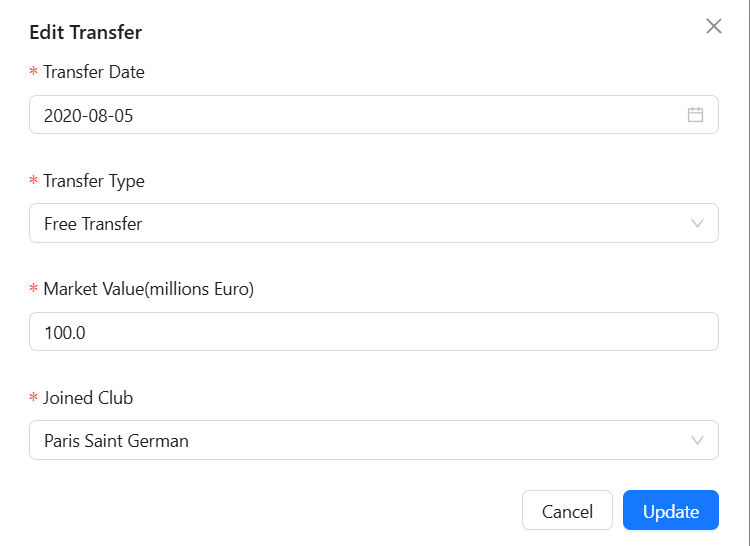
\includegraphics[width=1\linewidth]{Hinhve/admin_edit_transfer.png}
    \caption{Giao diện chỉnh sửa lịch sử chuyển nhượng}
    \label{fig:admin_edit_transfer}
\end{figure}
Giao diện chỉnh sửa chuyển nhượng như trên hình \ref{fig:admin_edit_transfer}. Admin có thể chỉnh sửa các thông tin chuyển nhượng của cầu thủ với các dạng khác nhau.

\subsection{Giao diện quản lý danh sách câu lạc bộ}
\begin{figure}
    \centering
    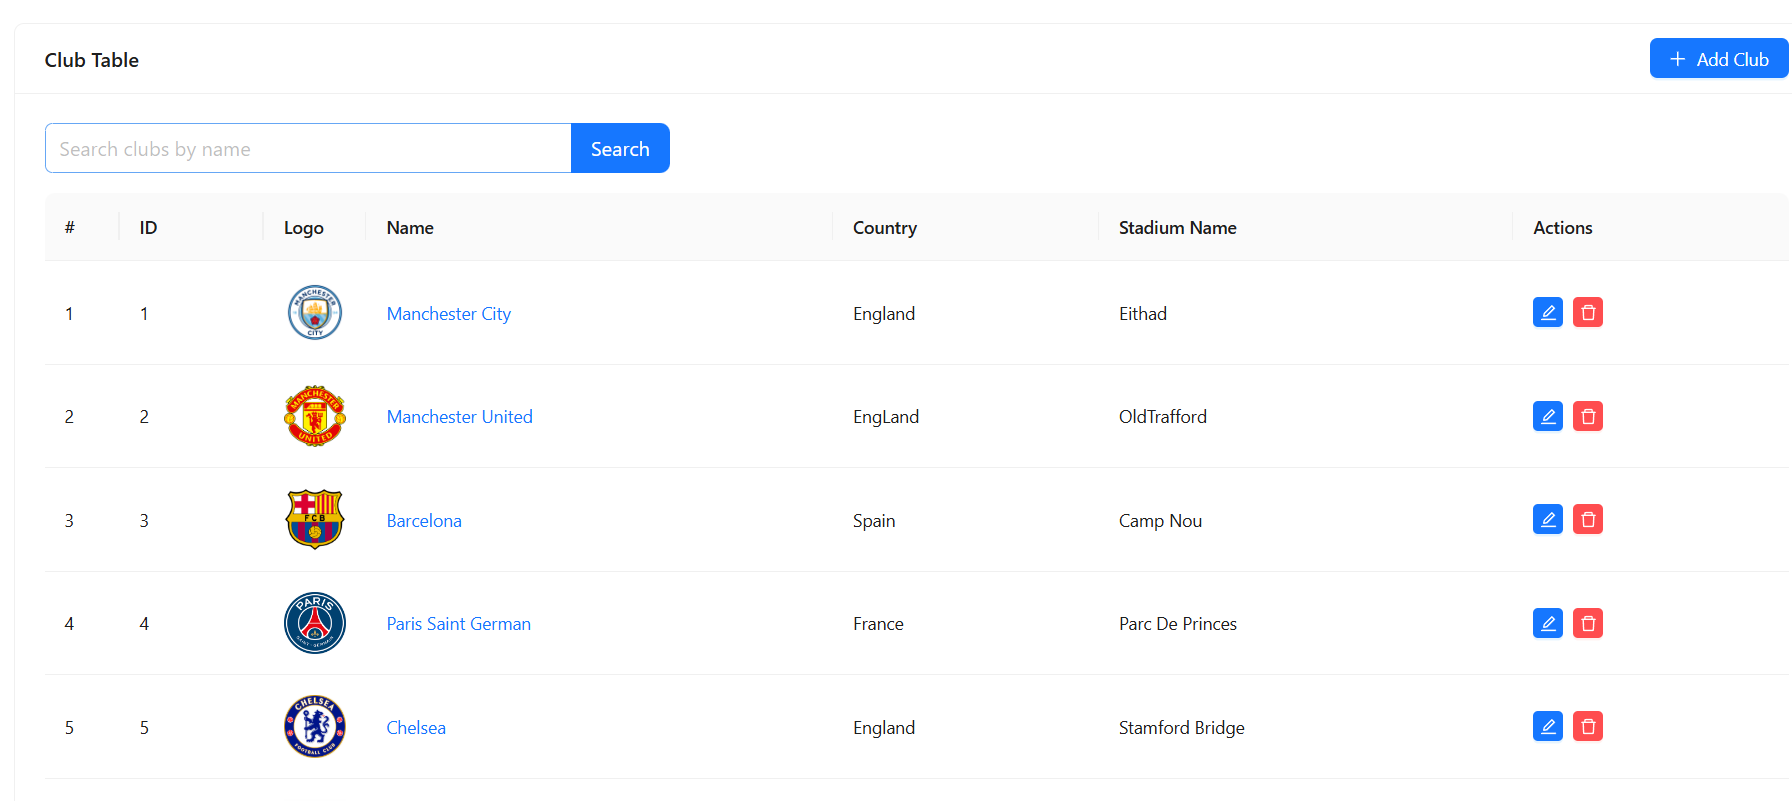
\includegraphics[width=1\linewidth]{Hinhve/admin_clubs.png}
    \caption{Giao diện quản lý danh sách câu lạc bộ}
    \label{fig:admin_clubs}
\end{figure}
Giao diện quản lý câu lạc bộ như trên hình \ref{fig:admin_clubs}. Giao diện hiển thị danh sách các câu lạc bộ cùng với thông tin và logo của từng đội.

\subsection{Giao diện tìm kiếm câu lạc bộ theo từ khoá}
\begin{figure}
    \centering
    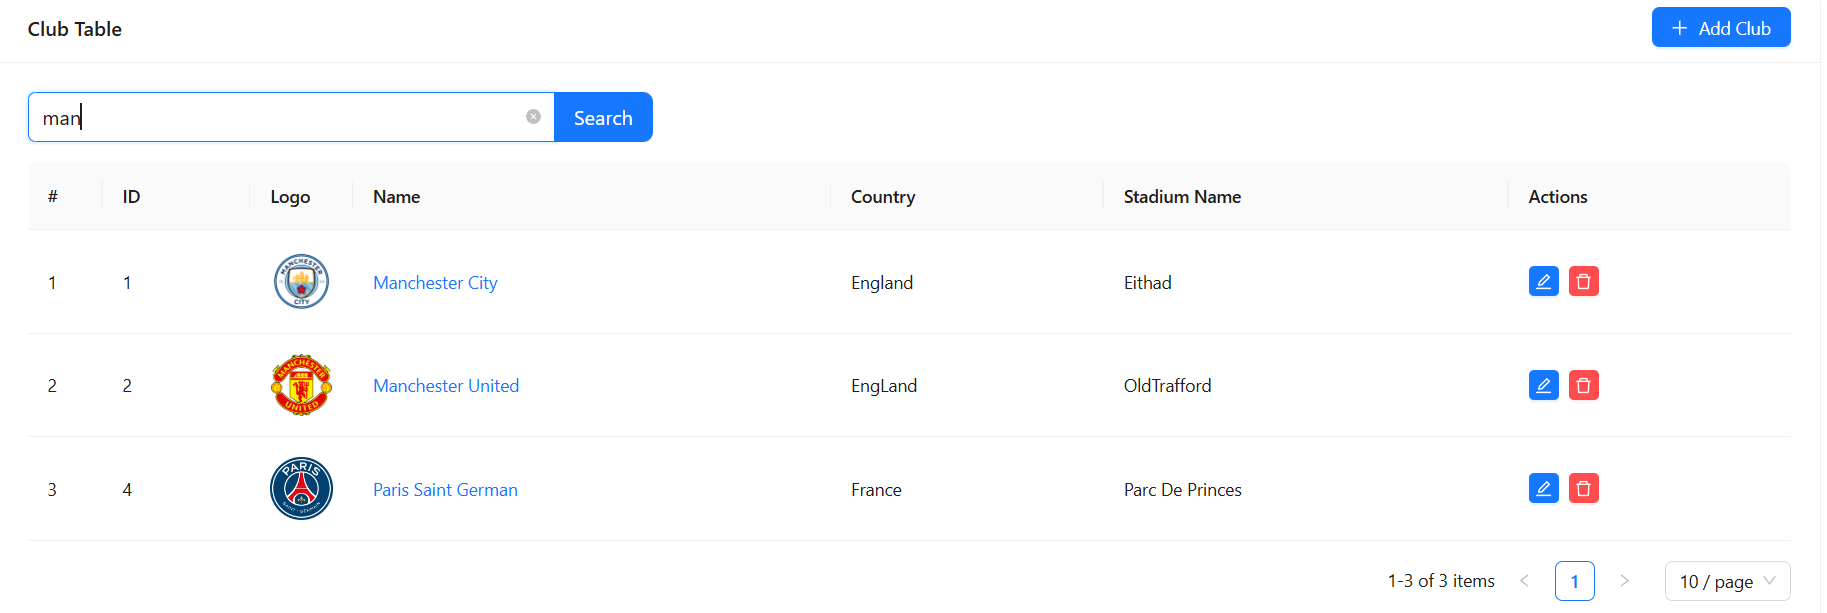
\includegraphics[width=1\linewidth]{Hinhve/admin_search_club.png}
    \caption{Giao diện tìm kiếm câu lạc bộ theo từ khoá}
    \label{fig:admin_search_club}
\end{figure}
Giao diện tìm kiếm câu lạc bộ như trên hình \ref{fig:admin_search_club}. Admin có thể nhập từ khóa để tìm kiếm nhanh các câu lạc bộ theo tên.

\subsection{Giao diện thêm mới câu lạc bộ}
\begin{figure}
    \centering
    \includegraphics[width=1\linewidth]{Hinhve/admin_add_club.png}
    \caption{Giao diện thêm mới câu lạc bộ}
    \label{fig:admin_add_club}
\end{figure}
Giao diện thêm mới câu lạc bộ như trên hình \ref{fig:admin_add_club}. Cho phép admin nhập tên, quốc gia, sân vận động và hình ảnh của câu lạc bộ mới.

\subsection{Giao diện chỉnh sửa thông tin câu lạc bộ}
\begin{figure}
    \centering
    \includegraphics[width=1\linewidth]{Hinhve/admin_edit_club.png}
    \caption{Giao diện chỉnh sửa thông tin câu lạc bộ}
    \label{fig:admin_edit_club}
\end{figure}
Giao diện chỉnh sửa câu lạc bộ như trên hình \ref{fig:admin_edit_club}. Admin có thể chỉnh sửa các thông tin của câu lạc bộ hiện có.

\subsection{Giao diện chi tiết thông tin câu lạc bộ}
\begin{figure}
    \centering  
    \includegraphics[width=1\linewidth]{Hinhve/admin_club_detail_v2.png}
    \caption{Giao diện chi tiết thông tin câu lạc bộ}
    \label{fig:admin_club_detail}
\end{figure}
Giao diện chi tiết câu lạc bộ như trên hình \ref{fig:admin_club_detail}. Admin có thể xem thông tin chi tiết của từng câu lạc bộ.

\subsection{Giao diện quản lý danh sách huấn luyện viên}
\begin{figure}
    \centering
    \includegraphics[width=1\linewidth]{Hinhve/admin_coaches.png}
    \caption{Giao diện quản lý danh sách huấn luyện viên}
    \label{fig:admin_coaches}
\end{figure}
Giao diện quản lý huấn luyện viên như trên hình \ref{fig:admin_coaches}. Hiển thị danh sách huấn luyện viên hiện có trong hệ thống.

\subsection{Giao diện tìm kiếm huấn luyện viên theo từ khoá}
\begin{figure}
    \centering
    \includegraphics[width=1\linewidth]{Hinhve/admin_search_coach.png}
    \caption{Giao diện tìm kiếm huấn luyện viên theo từ khoá}
    \label{fig:admin_search_coach}
\end{figure}
Giao diện tìm kiếm huấn luyện viên như trên hình \ref{fig:admin_search_coach}. Admin có thể nhập từ khóa để lọc HLV theo tên.

\subsection{Giao diện thêm mới huấn luyện viên}
\begin{figure}
    \centering
    \includegraphics[width=1\linewidth]{Hinhve/admin_add_coach.png}
    \caption{Giao diện thêm mới huấn luyện viên}
    \label{fig:admin_add_coach}
\end{figure}
Giao diện thêm mới huấn luyện viên như trên hình \ref{fig:admin_add_coach}. Admin nhập tên, tuổi, quốc gia và các thông tin liên quan để thêm huấn luyện viên mới.

\subsection{Giao diện chỉnh sửa thông tin huấn luyện viên}
\begin{figure}
    \centering
    \includegraphics[width=1\linewidth]{Hinhve/admin_edit_coach.png}
    \caption{Giao diện chỉnh sửa thông tin huấn luyện viên}
    \label{fig:admin_edit_coach}
\end{figure}
Giao diện chỉnh sửa huấn luyện viên như trên hình \ref{fig:admin_edit_coach}. Admin có thể cập nhật lại thông tin của HLV.

\subsection{Giao diện chi tiết thông tin huấn luyện viên}
\begin{figure}
    \centering
    \includegraphics[width=1\linewidth]{Hinhve/admin_coach_detail.png}
    \caption{Giao diện chi tiết thông tin huấn luyện viên}
    \label{fig:admin_coach_detail}
\end{figure}
Giao diện chi tiết huấn luyện viên như trên hình \ref{fig:admin_coach_detail}. Admin có thể nhấn vào từng huấn luyện viên để xem đầy đủ thông tin chi tiết về họ.


\subsection{Giao diện thêm mới lịch sử CLB}
\begin{figure}
    \centering
    \includegraphics[width=1\linewidth]{Hinhve/admin_add_club_history.png}
    \caption{Giao diện thêm mới lịch sử CLB}
    \label{fig:admin_add_club_history}
\end{figure}
Giao diện thêm mới lịch sử câu lạc bộ như hình \ref{fig:admin_add_club_history}. Admin có thể điền thông tin về các mốc lịch sử quan trọng trong quá khứ của câu lạc bộ.

\subsection{Giao diện chỉnh sửa lịch sử CLB}
\begin{figure}
    \centering
    \includegraphics[width=1\linewidth]{Hinhve/admin_edit_club_history.png}
    \caption{Giao diện chỉnh sửa lịch sử CLB}
    \label{fig:admin_edit_club_history}
\end{figure}
Giao diện chỉnh sửa lịch sử câu lạc bộ như hình \ref{fig:admin_edit_club_history}. Admin có thể cập nhật các thông tin đã lưu trước đó về lịch sử CLB.

\subsection{Giao diện bảng xếp hạng giải đấu}
\begin{figure}
    \centering
    \includegraphics[width=1\linewidth]{Hinhve/admin_league_table.png}
    \caption{Giao diện bảng xếp hạng giải đấu}
    \label{fig:admin_league_table}
\end{figure}
Giao diện bảng xếp hạng như hình \ref{fig:admin_league_table}. Hiển thị vị trí các đội bóng trong mùa giải hiện tại dựa trên kết quả thi đấu.

\subsection{Giao diện thêm mới giải đấu}
\begin{figure}
    \centering
    \includegraphics[width=1\linewidth]{Hinhve/admin_add_league.png}
    \caption{Giao diện thêm mới giải đấu}
    \label{fig:admin_add_league}
\end{figure}
Giao diện thêm giải đấu như hình \ref{fig:admin_add_league}. Admin nhập tên giải, quốc gia, mô tả và biểu tượng đại diện để thêm mới một giải đấu.

\subsection{Giao diện chỉnh sửa giải đấu}
\begin{figure}
    \centering
    \includegraphics[width=1\linewidth]{Hinhve/admin_edit_leauge.png}
    \caption{Giao diện chỉnh sửa giải đấu}
    \label{fig:admin_edit_league}
\end{figure}
Giao diện chỉnh sửa giải đấu như hình \ref{fig:admin_edit_league}. Cho phép admin cập nhật lại thông tin của một giải đã có.

\subsection{Giao diện chi tiết giải đấu}
\begin{figure}
    \centering
    \includegraphics[width=1\linewidth]{Hinhve/admin_league_detail.png}
    \caption{Giao diện chi tiết giải đấu}
    \label{fig:admin_league_detail}
\end{figure}
Giao diện chi tiết giải đấu như hình \ref{fig:admin_league_detail}. Hiển thị thông tin về giải đấu cùng các mùa giải đã và đang tổ chức.

\subsection{Giao diện thêm mới mùa giải}
\begin{figure}
    \centering
    \includegraphics[width=1\linewidth]{Hinhve/admin_add_season.png}
    \caption{Giao diện thêm mới mùa giải}
    \label{fig:admin_add_season}
\end{figure}
Giao diện thêm mùa giải như hình \ref{fig:admin_add_season}. Admin có thể chọn giải đấu liên quan, nhập tên mùa giải, năm diễn ra, mô tả và biểu tượng.

\subsection{Giao diện chỉnh sửa mùa giải}
\begin{figure}
    \centering
    \includegraphics[width=1\linewidth]{Hinhve/admin_edit_season.png}
    \caption{Giao diện chỉnh sửa mùa giải}
    \label{fig:admin_edit_season}
\end{figure}
Giao diện chỉnh sửa mùa giải như hình \ref{fig:admin_edit_season}. Cho phép admin cập nhật lại thông tin về mùa giải hiện tại hoặc trước đó.

\subsection{Giao diện thêm CLB vào mùa giải}
\begin{figure}
    \centering
    \includegraphics[width=1\linewidth]{Hinhve/admin_add_club_season_v2.png}
    \caption{Giao diện thêm CLB vào mùa giải}
    \label{fig:admin_add_club_season}
\end{figure}
Giao diện thêm câu lạc bộ vào mùa giải như hình \ref{fig:admin_add_club_season}. Admin chọn các CLB sẽ tham gia mùa giải cụ thể.

\subsection{Giao diện chỉnh sửa thống kê CLB theo mùa}
\begin{figure}
    \centering
    \includegraphics[width=1\linewidth]{Hinhve/admin_edit_club_season_v2.png}
    \caption{Giao diện chỉnh sửa thống kê CLB theo mùa}
    \label{fig:admin_edit_club_season}
\end{figure}
Giao diện chỉnh sửa thống kê CLB theo mùa như hình \ref{fig:admin_edit_club_season}. Admin có thể cập nhật thông tin số trận, số bàn, thẻ, thứ hạng,... của từng CLB trong mùa giải.


\subsection{Giao diện danh sách trận đấu trong mùa giải}
\begin{figure}
    \centering
    \includegraphics[width=1\linewidth]{Hinhve/admin_matches.png}
    \caption{Giao diện danh sách trận đấu trong mùa giải}
    \label{fig:admin_matches}
\end{figure}
Giao diện danh sách các trận đấu đã được tạo cho mùa giải như hình \ref{fig:admin_matches}. Admin có thể tạo mới hoặc sửa thông tin trận đấu tại đây.

\subsection{Giao diện quản lý danh sách trận đấu}
\begin{figure}
    \centering
    \includegraphics[width=1\linewidth]{Hinhve/admin_add_match.png}
    \caption{Giao diện quản lý danh sách trận đấu}
    \label{fig:admin_add_match}
\end{figure}
Giao diện thêm mới các trận đấu trong hệ thống như hình \ref{fig:admin_add_match}. 

\subsection{Giao diện chỉnh sửa trận đấu}
\begin{figure}
    \centering
    \includegraphics[width=1\linewidth]{Hinhve/admin_edit_match.png}
    \caption{Giao diện chỉnh sửa trận đấu}
    \label{fig:admin_edit_match}
\end{figure}
Giao diện chỉnh sửa thông tin một trận đấu cụ thể như hình \ref{fig:admin_edit_match}. Admin có thể thay đổi thời gian, địa điểm, đội tham gia,...

\subsection{Giao diện chi tiết trận đấu}
\begin{figure}
    \centering
    \includegraphics[width=1\linewidth]{Hinhve/admin_match_actions.png}
    \caption{Giao diện chi tiết trận đấu}
    \label{fig:admin_match_actions}
\end{figure}
Giao diện hiển thị chi tiết trận đấu như hình \ref{fig:admin_match_actions}. Bao gồm thông tin đội, tỉ số, cầu thủ ghi bàn, thẻ phạt,...

\subsection{Giao diện thêm mới hành động trong trận}
\begin{figure}
    \centering
    \includegraphics[width=1\linewidth]{Hinhve/admin_add_match_action.png}
    \caption{Giao diện thêm mới hành động trong trận}
    \label{fig:admin_add_match_action}
\end{figure}
Giao diện thêm hành động (như bàn thắng, thẻ vàng,...) trong trận đấu như hình \ref{fig:admin_add_match_action}. Admin chọn cầu thủ, thời điểm và loại hành động.

\subsection{Giao diện chỉnh sửa hành động trong trận}
\begin{figure}
    \centering
    \includegraphics[width=1\linewidth]{Hinhve/admin_edit_match_action.png}
    \caption{Giao diện chỉnh sửa hành động trong trận}
    \label{fig:admin_edit_match_action}
\end{figure}
Giao diện chỉnh sửa thông tin các hành động đã xảy ra trong trận đấu như hình \ref{fig:admin_edit_match_action}. Cho phép chỉnh thời gian, loại hành động hoặc cầu thủ liên quan.

\section{ Ứng dụng bảo mật cho Website}

\subsection{JWT}
Nhóm em sử dụng JWT để bảo mật hơn cho BTL website của nhóm. 
\subsubsection{ Lý thuyết}
JSON Web Token (JWT) là một tiêu chuẩn được sử dụng để truyền thông tin an toàn giữa máy khách (như ứng dụng frontend) và máy chủ (backend). JWT thường được sử dụng để xác minh danh tính người dùng, xác thực họ, và đảm bảo giao tiếp an toàn giữa hai bên. JWT chủ yếu được sử dụng trong các ứng dụng web và API để bảo vệ khỏi truy cập trái phép.\cite{jwt-gfg}

Dữ liệu trong JWT, chẳng hạn như thông tin người dùng, được lưu trữ dưới định dạng JSON đơn giản. Để giữ an toàn cho dữ liệu, token được ký mã hóa, đảm bảo rằng không ai có thể thay đổi nó. Việc ký có thể được thực hiện bằng các phương pháp mã hóa sau:

\begin{itemize}
    \item HMAC (Mã xác thực thông điệp dựa trên hàm băm)
    \item RSA hoặc ECDSA (Thuật toán mã hóa bất đối xứng)
\end{itemize}
JWT chủ yếu được sử dụng cho việc xác thực và trao đổi dữ liệu an toàn trong các ứng dụng web và API.

Cách JWT token hoạt động như sau:
\begin{itemize}
    \item Người dùng đăng nhập: Máy khách (trình duyệt) gửi thông tin đăng nhập đến máy chủ.
    \item Máy chủ tạo JWT: Nếu thông tin đăng nhập hợp lệ, máy chủ tạo JWT chứa dữ liệu người dùng và ký nó bằng khóa bí mật.
    \item Token được gửi cho máy khách: JWT được gửi lại cho máy khách và lưu trữ (thường trong localStorage hoặc cookie).
    \item Máy khách gửi token trong các yêu cầu: Đối với các đường dẫn được bảo vệ, máy khách kèm JWT trong header Authorization (Bearer Token).
    \item Máy chủ xác minh và phản hồi: Máy chủ xác minh token, trích xuất thông tin người dùng, và xử lý yêu cầu nếu hợp lệ.
\end{itemize}

Token được sử dụng để truyền an toàn thông tin nhạy cảm giữa máy khách và máy chủ. Thay vì gửi dữ liệu thô (ví dụ: thông tin người dùng) có thể bị giả mạo, token cung cấp một phương thức xác thực an toàn. JWT được áp dụng rộng rãi vì chúng không thể bị can thiệp, đảm bảo dữ liệu không bị thay đổi trong quá trình truyền.

Việc sử dụng JWT có ứng dụng tương đối tốt trong việc bảo mật web như:
\begin{itemize}
    \item Sử dụng HTTPS: Ngăn chặn tấn công man-in-the-middle bằng cách truyền JWT qua HTTPS.
    \item Đặt thời gian hết hạn: Ngăn chặn token tồn tại quá lâu có thể bị khai thác.
    \item Sử dụng lưu trữ an toàn: Lưu trữ JWT an toàn (ví dụ: cookie HttpOnly thay vì local storage - bộ nhớ máy tính người dùng).
    \item Xác minh chữ ký: Luôn xác thực chữ ký của token trước khi tin tưởng nội dung của nó.
\end{itemize}
\subsubsection{ Cài đặt}
Đầu tiên là cấu hình bảo mật trong file SecurityConfig để sử dụng JWT:
\begin{lstlisting}[language=Java]
@Configuration
@EnableMethodSecurity(securedEnabled = true)
public class SecurityConfig {
    @Value("${jwt.base64-secret}")
    private String jwtKey;
    
    @Bean
    public SecurityFilterChain filterChain(HttpSecurity http, CustomAuthenticationEntryPoint customAuthenticationEntryPoint) throws Exception {
        String[] whiteList = {
                "/",
                "/api/v1/auth/login", "/api/v1/auth/refresh", "/api/v1/auth/register",
                "/storage/**",
                "/v3/api-docs/**",
                "/swagger-ui/**",
                "/swagger-ui.html"
        };
        http
                .csrf(AbstractHttpConfigurer::disable)
                .cors(Customizer.withDefaults())
                .authorizeHttpRequests(
                        authz -> authz
                                .requestMatchers(whiteList).
                        permitAll()
                                .anyRequest().authenticated())
                .oauth2ResourceServer((oauth2) -> oauth2.jwt(Customizer.withDefaults())
                        .authenticationEntryPoint
                    (customAuthenticationEntryPoint));
        return http.build();
    }
}
\end{lstlisting}

Tiếp theo là viết các hàm giúp tạo JWT Token, giải mã và lấy thông tin người dùng trong file SecurityConfig, tạo Access token và refresh token. Access token chứa thông tin cơ bản của người dùng và quyền hạn, được sử dụng cho hầu hết các yêu cầu API. Refresh token có thời hạn dài hơn và được sử dụng để tạo mới access token khi nó hết hạn mà không yêu cầu người dùng đăng nhập lại. Hệ thống sử dụng NimbusJwtDecoder để giải mã và xác thực token với cùng một khóa bí mật đã dùng để tạo token. Và cuối cùng viết lớp CustomAuthenticationEntryPoint, lớp này xử lý các lỗi xác thực, trả về thông báo lỗi với định dạng JSON khi token không hợp lệ hoặc hết hạn.
\section{ Hướng đẫn triển khai trên Render}
Sau khi đẩy Docker image lên Docker Hub, trên Docker Hub sẽ như trên hình \ref{fig:dockerhub}. Tiếp theo truy cập \href{https://dashboard.render.com/}{Render}, tạo tài khoản, tạo dự án và nhấn tạo Web Service như trên hình \ref{fig:render-create-web-service}. Giao diện tạo dịch vụ web như trên hình \ref{fig:render-web-service-existing-imag}, nhấn chọn Existing Image rồi sau đó nhập docker.io/dockerhub\_username/docker\_image\_name, trong đó dockerhub\_username là tên tài khoản Docker hub, docker\_image\_name là tên image đẩy lên Docker hub. Sau đó chọn loại instance tương ứng như trên hình \ref{fig:render-choose-instance}. Tiếp theo sẽ khai báo các biến môi trường ví dụ như API Key, password mà không muốn công khai trên mạng, sau khi nhập xong giao diện sẽ như hình \ref{fig:render-environment-variable}. Rồi sau đó connect và chờ một thời gian để Render chạy dịch vụ, sau khi chạy xong thì ta đã triển khai thành công trên Render.

\begin{figure}
    \centering
    \includegraphics[width=1\linewidth]{Hinhve/dockerhub.png}
    \caption{Docker image trên Dockerhub}
    \label{fig:dockerhub}
\end{figure}

\begin{figure}
    \centering
    \includegraphics[width=1\linewidth]{Hinhve/render-create-web-service.png}
    \caption{Giao diện tạo Web Service của Render}
    \label{fig:render-create-web-service}
\end{figure}
\begin{figure}
    \centering
    \includegraphics[width=1\linewidth]{Hinhve/render-web-service-existing-image.png}
    \caption{ Giao diện tạo web service từ Docker image trên Dockerhub}
    \label{fig:render-web-service-existing-imag}
\end{figure}
\begin{figure}
    \centering
    \includegraphics[width=1\linewidth]{Hinhve/render-choose-instance.png}
    \caption{Giao diện chọn loại instance trên Render}
    \label{fig:render-choose-instance}
\end{figure}
\begin{figure}
    \centering
    \includegraphics[width=1\linewidth]{Hinhve/render-environment-variable.png}
    \caption{Giao diện nhập các biến môi trường}
    \label{fig:render-environment-variable}
\end{figure}
\end{document}